\documentclass[11pt,a4paper,onecolumn]{article}
%
\usepackage[top=30truemm,bottom=30truemm,left=25truemm,right=25truemm]{geometry}
\usepackage{amsmath,amssymb}
\makeatletter
\@addtoreset{equation}{section}
\def\theequation{\thesection.\arabic{equation}}
\makeatother
\makeatletter
\@addtoreset{table}{section}
\def\thetable{\thesection.\arabic{table}}
\makeatother
\usepackage{bm}
\usepackage[dvipdfmx]{graphicx}
\usepackage{ascmac}
\usepackage{longtable}
\usepackage{booktabs}
\usepackage{ltablex,booktabs}
\usepackage[dvipdfm,hidelinks]{hyperref}

\AtBeginDocument{
  \abovedisplayskip     =1.2\abovedisplayskip
  \abovedisplayshortskip=1.2\abovedisplayshortskip
  \belowdisplayskip     =1.2\belowdisplayskip
  \belowdisplayshortskip=1.2\belowdisplayshortskip}

\makeatletter
\def\maxwidth{\ifdim\Gin@nat@width>\linewidth\linewidth\else\Gin@nat@width\fi}
\def\maxheight{\ifdim\Gin@nat@height>\textheight\textheight\else\Gin@nat@height\fi}
\makeatother
% Scale images if necessary, so that they will not overflow the page
% margins by default, and it is still possible to overwrite the defaults
% using explicit options in \includegraphics[width, height, ...]{}
\setkeys{Gin}{width=\maxwidth,height=\maxheight,keepaspectratio}
%
\title{\Huge Description for MATSIRO6}
\author{}
\date{\today}
\pagenumbering{arabic}
%
%
%
\begin{document}
%
	\maketitle
	\tableofcontents
	\clearpage
	%
	\def\tightlist{\itemsep1pt\parskip0pt\parsep0pt}
	\hypertarget{introduction}{%
\section{Introduction}\label{introduction}}

Minimal Advanced Treatments of Surface Interaction and RunOff (MATSIRO) is a land surface parameterization originally formulated in the early 2000's (Takata et al., 2003) to produce terrestrial
boundary condition of the atmospheric general circulation model developed by the Center for Climate System Research at the University of Tokyo and the National Institute for Environmental Studies
(CCSR/NIES AGCM), as well as to other global climate models. It was originally designed to be primarily used for integration of climate simulations such as those involving long time scales from one
month to several hundred years coupled with the atmospheric model at grid resolutions of tens of kilometers or more. The main objective in its development was to represent all of the important water
and energy exchange processes between land and atmosphere as fully and accurately as possible (i.e., advanced treatment) in such time and spatial scales, while modeling them as simply as possible
(i.e., minimal treatment) so as to allow the results to be easily interpreted.

At the very early stage (2000's), when the first description was written by Emori (Emori, 2001), MATSIRO was developed based on the land surface submodel of CCSR/NIES AGCM5.4g coupled with the
parameterization for a vegetated surface (canopy) by Watanabe (1994), while at the same time improving certain processes such as those related to snow and runoff. Subsequently, with modifications in
the structure of AGCM, changes were made dealing with flux couplers and parallel processing so as to make it compatible with AGCM5.6. With regard to the physiological processes of vegetation, a
Jarvis-type function was initially used for stomatal resistance. Later, however, the Farquhar-type photosynthesis scheme, which served as a de facto standard in the world due to the progress of
studies on climate-ecosystem interactions at that time, was ported from SiB2 code.

Since then, MATSIRO has been used in CCSR/NIES/FRCGC AGCM5.7, which is adopted by an atmosphere-ocean coupled model MIROC3 (K-1 model developers, 2004), and MIROC5 (Watanabe et al., 2010) with only
minor model updates and bug fixes. Instead, during these times, MATSIRO had been intensively used with so-called offline setting (i.e., without coupling with the atmospheric model, but forced with
given surface atmospheric forcings) with original updates and improvements of some processes. Such efforts generate some branches of the model, called MAT-GW (water table depth dynamics; Koirala et
al.~2014), HiGW-MAT (coupled with anthropogenic activity and groundwater; Pokhrel et al.~2015), IsoMATSIRO (stable water isotopes included; Yoshimura et al., 2006). MATSIRO also has been validated and
compared with other land surface parameterizations under some international protocols like PILPS, GSWP, and ISIMIP. By these attempts, it was revealed that, apart from its original design, MATSIRO was
able to be used for higher resolution (up to about 1 kilometer) and shorter time scales (subdaily), so that MATSIRO is now used for short-term flood prediction over Japan with a new hydro-dynamical
model, CaMa-Flood (Yamazaki et al., 2011), for example (Ma et al., 2021).

Here, with development of MIROC6 (Tatebe et al., 2019), MATSIRO adopted significant model updates, so we decided to update its description for the first time since 2001. We named this version of
MATSIRO as MATSIRO6. Major and minor updates in this document are as follows:

\begin{itemize}
\tightlist
\item
  Snow cover fraction diagnosis (Chapter 8)
\item
  Runoff representation (Chapter 9)
\item
  Lake process coupled with river (Chapter 11)
\item
  Snow-fed wetland process (Chapter 12)
\item
  Tiling with lake, cropland, and natural vegetation (Chapter 13)
\end{itemize}

It should be noted that even though river routing process is also implemented in MIROC6 and other versions, this document does not include description of river process.

\hypertarget{structure}{%
\subsection{Structure}\label{structure}}

MATSIRO consists of flux calculation section and land integration section. In the flux calculation section, the calculations are conducted separately for snow-covered and snow-free potions. For each
snow-free portion (\(l=1\)) and snow-covered portion (\(l=2\)), the subroutines for various processes are called, the fluxes are calculated, and the ground surface temperature and canopy temperature
are updated. Specifically, the following subroutines are called in the order shown below:

\begin{enumerate}
\def\labelenumi{(\alph{enumi})}
\tightlist
\item
  MATLAI: vegetation type parameter (LAI, vegetation height) set
\item
  MATRAD: calculation of radiation parameters (albedo, vegetation transmissivity, etc.)
\item
  MATBLK: calculation of turbulence parameters (bulk coefficients)
\item
  MATRST: calculation of stomatal resistance, bare soil surface evaporation resistance, etc.
\item
  MATFLX: calculation of surface flux
\item
  MATGHC: calculation of ground heat conduction
\item
  MATSHB: solution of surface heat balance
\end{enumerate}

Then, fluxes from lake surface are calculated separately for ice-covered and ice-free portions. The following subroutines are called in the order shown below:

\begin{enumerate}
\def\labelenumi{(\alph{enumi})}
\setcounter{enumi}{7}
\tightlist
\item
  LAKEBC: calculation of lake surface conditions (albedo, roughness, etc.)
\item
  SFCFLX: calculation of surface flux
\item
  RADSFC: calculation of radiation flux (downward and upward shortwave radiation)
\item
  LAKEHB: solution of energy balance at lake surface
\end{enumerate}

In the land integration section, the subroutines for various processes are called and land surface prognostic variables are updated. Specifically, the following subroutines are called in the order
shown below:

\begin{enumerate}
\def\labelenumi{(\alph{enumi})}
\setcounter{enumi}{11}
\tightlist
\item
  MATCNW: calculation of canopy water balance
\item
  MATSNW: calculation of snow water equivalent, snow temperature, and snow albedo
\item
  MATROF: calculation of runoff
\item
  MATGND: calculation of soil temperature, soil moisture, and frozen soil
\end{enumerate}

Finally, the lake modules are called and the related prognostic variables are updated.

\begin{enumerate}
\def\labelenumi{(\alph{enumi})}
\setcounter{enumi}{15}
\tightlist
\item
  SETSCNV: calculation of convergence of shortwave radiation
\item
  LAKEIC: calculation of lake ice
\item
  LAKEPO: calculation of lake water and temperature
\item
  PUTDEFF: sending a lake water deficit for the lakes whose water levels are below the lower limit
\end{enumerate}

\hypertarget{prognostic-variables}{%
\subsection{Prognostic variables}\label{prognostic-variables}}

MATSIRO has the following prognostic variables for each tile:

\begin{longtable}[]{@{}lll@{}}
\caption{Prognostic variables}\tabularnewline
\toprule
Variable & Description & Units \\
\midrule
\endfirsthead
\toprule
Variable & Description & Units \\
\midrule
\endhead
\(T_{s(l)}\) \((l=1,2)\) & Ground surface temperature & \(\mathrm{[K]}\) \\
\(T_{c(l)}\) \((l=1,2)\) & Canopy temperature & \(\mathrm{[K]}\) \\
\(T_{g(k)}\) \((k=1,\ldots,K_g)\) & Soil temperature & \(\mathrm{[K]}\) \\
\(w_{(k)}\) \((k=1,\ldots,K_g)\) & Soil moisture content & \(\mathrm{[m^3/m^3]}\) \\
\(w_{i(k)}\) \((k=1,\ldots,K_g)\) & Frozen soil moisture content & \(\mathrm{[m^3/m^3]}\) \\
\(w_c\) & Water content on the canopy & \(\mathrm{[m]}\) \\
\(Sn\) & Snow water equivalent & \(\mathrm{[kg/m^2]}\) \\
\(T_{Sn(k)}\) \((k=1,\ldots,K_{Sn})\) & Snow temperature & \(\mathrm{[K]}\) \\
\(\alpha_{Sn(b)}\) \((b=1,2,3)\) & Snow albedo & \(\mathrm{[-]}\) \\
\(A_{Sn}\) & Snow cover fraction & \(\mathrm{[-]}\) \\
\(\mu\) & Accumulated snowfall & \(\mathrm{[kg/m^2]}\) \\
\(D_m\) & Accumulated snowmelt & \(\mathrm{[kg/m^2]}\) \\
\(R_{sn}\) & Reset flag for snow accumulation or ablation season & \(\mathrm{[-]}\) \\
\(I_{sn}\) & Snow index & \(\mathrm{[-]}\) \\
\(A_{L}\) & Land cover fraction & \(\mathrm{[-]}\) \\
\(T_{hist}\) & Long-term mean temperature & \(\mathrm{[K]}\) \\
\(\rho_d\) & Dust density in snow & \(\mathrm{[ppmw]}\) \\
\(\rho_d\) & Dust density in snow (mass) & \(\mathrm{[ppmw]}\) \\
\(\alpha_{ice(b)}\) & Ice albedo & \(\mathrm{[-]}\) \\
\bottomrule
\end{longtable}

where \(l=1,2\) denotes snow-free and snow-covered portions, respectively; \(k\) is the vertical layer number of the soil or snow (the uppermost layer is 1, with the number increasing as the layer
becomes deeper); \(K_g\) is the number of soil layers; \(K_{Sn}\) is the number of snow layers; and \(b=1,2,3\) denotes the bands of visible, near infrared, and infrared wavelengths, respectively.

As the default setting, the soil has six layers whose thicknesses are defined by the depth boundaries of 5, 20, 75, 100, 200, and 1000 cm from the surface. The definition points of soil temperature,
soil moisture, and frozen soil moisture are the same. The maximum number of snow layer is three by default, while the number is diagnosed from snow water equivalent. As the default setting, the
maximum number is three layers.

The ground surface temperature and canopy temperature are so-called surface temperatures whose heat capacity is zero; however, they take the form of prognostic variables. (The current calculation
method depends on the values of the preceding step because the stability, etc. assessed by the values of the preceding step are used. If the stability, etc. were to be assessed by updated values and
calculation iterated to the point of convergence, perfect diagnostic variables would be obtained that would not depend on the values of the preceding step.) The other variables are all prognostic
variables that always require the values of the preceding step.

The ground surface temperature and canopy temperature are updated in the flux calculation section. All of the other variables (original prognostic variables) are updated in the land surface
integration section.

The lake part has the following prognostic variables:

\begin{longtable}[]{@{}lll@{}}
\caption{Prognostic variables for the lake scheme}\tabularnewline
\toprule
Variable & Description & Units \\
\midrule
\endfirsthead
\toprule
Variable & Description & Units \\
\midrule
\endhead
\(T\) & Lake temperature & \(\mathrm{[^{\circ}C]}\) \\
\(S\) & Lake salinity & \(\mathrm{[PSU]}\) \\
\(T_I\) & Lake ice surface temperature & \(\mathrm{[^{\circ}C]}\) \\
\(A_I\) & Lake ice concentration & \(\mathrm{[-]}\) \\
\(h_I\) & Mean lake ice thickness over ice-covered part of a grid & \(\mathrm{[cm]}\) \\
\(h_S\) & Mean snow depth over lake ice & \(\mathrm{[cm]}\) \\
\(h\) & Lake level & \(\mathrm{[cm]}\) \\
\bottomrule
\end{longtable}

\hypertarget{input-data}{%
\subsection{Input data}\label{input-data}}

The following variables are input in the flux calculation section:

\begin{longtable}[]{@{}lll@{}}
\caption{Input data for land flux calculation}\tabularnewline
\toprule
Variable & Description & Units \\
\midrule
\endfirsthead
\toprule
Variable & Description & Units \\
\midrule
\endhead
\(u_a\) & Atmospheric 1st layer eastward wind & \(\mathrm{[m/s]}\) \\
\(v_a\) & Atmospheric 1st layer northward wind & \(\mathrm{[m/s]}\) \\
\(T_a\) & Atmospheric 1st layer temperature & \(\mathrm{[K]}\) \\
\(q_a\) & Atmospheric 1st layer specific humidity & \(\mathrm{[kg/kg]}\) \\
\(P_a\) & Atmospheric 1st layer pressure & \(\mathrm{[Pa]}\) \\
\(P_s\) & Surface pressure & \(\mathrm{[Pa]}\) \\
\(R^{\downarrow}_{(d,b)}\) \((d=1,2;b=1,2,3)\) & Surface downward radiation flux & \(\mathrm{[W/m^2]}\) \\
\bottomrule
\end{longtable}

where \(d=1,2\) denotes direct and diffuse, respectively; and \(b=1,2,3\) denotes the bands of visible, near infrared, and infrared wavelengths, respectively.

The following variables are input in the land surface integration section:

\begin{longtable}[]{@{}lll@{}}
\caption{Input data for land integration section}\tabularnewline
\toprule
Variable & Description & Units \\
\midrule
\endfirsthead
\toprule
Variable & Description & Units \\
\midrule
\endhead
\(Pr_{c}\) & Convective rainfall flux & \(\mathrm{[kg/m^2/s]}\) \\
\(Pr_{l}\) & Large-scale Rainfall flux & \(\mathrm{[kg/m^2/s]}\) \\
\(P_{Snc}\) & Convective snowfall flux & \(\mathrm{[kg/m^2/s]}\) \\
\(P_{Snl}\) & Large-scale snowfall flux & \(\mathrm{[kg/m^2/s]}\) \\
\(F_{g(1/2)}\) & Surface heat transfer flux & \(\mathrm{[W/m^2]}\) \\
\(F_{Sn(1/2)}\) & Heat transfer flux for snow surface & \(\mathrm{[W/m^2]}\) \\
\(Et_{(i,j)}\) \((i=1,2;j=1,2,3)\) & Evapotranspiration & \(\mathrm{[kg/m^2/s]}\) \\
\(\Delta F_{conv}\) & Surface energy convergence & \(\mathrm{[W/m^2]}\) \\
\(F_{root(k)}\) \((k=1,\ldots,K_g)\) & Root water uptake & \(\mathrm{[kg/m^2/s]}\) \\
\(LAI\) & Leaf area index & \(\mathrm{[m^2/m^2]}\) \\
\(A_{Snc}\) & Canopy freezing area ratio & \(\mathrm{[-]}\) \\
\(D_{dust}\) & Dust deposition flux & \(\mathrm{[kg/m^2/s]}\) \\
\(D_{BC}\) & Black carbon deposition flux & \(\mathrm{[kg/m^2/s]}\) \\
\bottomrule
\end{longtable}

\hypertarget{output-data}{%
\subsection{Output data}\label{output-data}}

The following variables are output from the flux calculation section:

\begin{longtable}[]{@{}lll@{}}
\caption{Output data from the flux calculation section}\tabularnewline
\toprule
Variable & Description & Units \\
\midrule
\endfirsthead
\toprule
Variable & Description & Units \\
\midrule
\endhead
\(\tau_x\) & Surface eastward wind stress & \(\mathrm{[N/m^2]}\) \\
\(\tau_y\) & Surface northward wind stress & \(\mathrm{[N/m^2]}\) \\
\(H\) & Sensible heat flux & \(\mathrm{[W/m^2]}\) \\
\(E\) & Latent heat flux & \(\mathrm{[kg/m^2/s]}\) \\
\(R^{\uparrow}_S\) & Upward shortwave radiation flux & \(\mathrm{[W/m^2]}\) \\
\(R^{\uparrow}_L\) & Upward longwave radiation flux & \(\mathrm{[W/m^2]}\) \\
\(\alpha_{s(b)}\) \((b=1,2,3)\) & Surface albedo & \(\mathrm{[-]}\) \\
\(T_{sR}\) & Surface radiation temperature & {[}K{]} \\
\(F_{g(1/2)}\) & Surface heat transfer flux & \(\mathrm{[W/m^2]}\) \\
\(F_{Sn(1/2)}\) & Heat transfer flux for snow surface & \(\mathrm{[W/m^2]}\) \\
\(Et_{(i,j)}\) \((i=1,2;j=1,2,3)\) & Evapotranspiration & \(\mathrm{[kg/m^2/s]}\) \\
\(\Delta F_{conv}\) & surface energy convergence & \(\mathrm{[W/m^2]}\) \\
\(F_{root(k)}\) \((k=1,\ldots,K_g)\) & Root sucking flux & \(\mathrm{[kg/m^2/s]}\) \\
\(LAI\) & leaf area index & \(\mathrm{[m^2/m^2]}\) \\
\(A_{Snc}\) & Canopy freezing area ratio & \(\mathrm{[-]}\) \\
\bottomrule
\end{longtable}

where \(i=1,2\) denotes liquid and solid evapotranspiration, respectively; and \(j=1,2,3\) denotes evaporation from the bare soil surface (forest floor), transpiration, and canopy water evaporation,
respectively. Other indexes are the same as described earlier.

The following variable is output from the land surface integration section:

\begin{longtable}[]{@{}lll@{}}
\caption{Output data}\tabularnewline
\toprule
Variable & Description & Units \\
\midrule
\endfirsthead
\toprule
Variable & Description & Units \\
\midrule
\endhead
\(Ro\) & runoff & \(\mathrm{[kg/m^2/s]}\) \\
\bottomrule
\end{longtable}

Runoff is used as an input variable for the river channel network model.

\hypertarget{external-parameters}{%
\subsection{External parameters}\label{external-parameters}}

The external parameters necessary for the execution of MATSIRO are broadly divided into two types: parameters whose values for each grid cell are given by horizontal distribution (map), and parameters
whose values are given by land cover type or soil type tables. The land cover types and soil types are the parameters given by map, and through this, each parameter given by table is allocated to
individual grid cells; that is,

parameter given by a map: \begin{eqnarray}
 \phi(i,j)
\end{eqnarray}

parameter given by a table: \begin{eqnarray}
 \psi(I),
\end{eqnarray} \begin{eqnarray}
 I = I_L (i,j)
\end{eqnarray} or \begin{eqnarray}
 I = I_S (i,j)
\end{eqnarray} where \((i,j)\) are indexes of the grid horizontal location, \(I_L\) is the land use type, and \(I_S\) is the soil type.

The types of external parameters \(\phi\) given by map are as follows:

\begin{longtable}[]{@{}llll@{}}
\caption{External parameters given by maps}\tabularnewline
\toprule
Variable & Description & Temporal resolution & Units \\
\midrule
\endfirsthead
\toprule
Variable & Description & Temporal resolution & Units \\
\midrule
\endhead
\(I_L\) & Land cover type & constant & \(\mathrm{[-]}\) \\
\(I_S\) & Soil Type & constant & \(\mathrm{[-]}\) \\
\(LAI_0\) & Leaf Area Index (LAI) & every month & \(\mathrm{[m^2/m^2]}\) \\
\(\alpha_{0(b)}\) \((b=1,2,3)\) & Ground surface (forest floor) albedo & constant & \(\mathrm{[-]}\) \\
\(\tan\beta_{s}\) & Tangent of the mean surface slope & constant & \(\mathrm{[-]}\) \\
\(\sigma_z\) & elevation standard deviation & constant & \(\mathrm{[m]}\) \\
\bottomrule
\end{longtable}

The types of external parameters \(\psi\) given by table for each land cover type are as follows:

\begin{landscape}

\begin{longtable}[]{@{}lll@{}}
\caption{External parameters given by tables}\tabularnewline
\toprule
Variable & Description & Units \\
\midrule
\endfirsthead
\toprule
Variable & Description & Units \\
\midrule
\endhead
\(h_0\) & vegetation height & \(\mathrm{[m]}\) \\
\(h_{B0}\) & Height of the bottom of the canopy & \(\mathrm{[m]}\) \\
\(r_{f(b)}\) (\(b\)=1,2) & Leaf albedo & \(\mathrm{[-]}\) \\
\(t_{f(b)}\) (\(b\)=1,2) & Leaf transmissivity & \(\mathrm{[-]}\) \\
\(f_{root(k)}\) (\(k=1,\ldots,K_g\)) & Percentage of root presence & \(\mathrm{[-]}\) \\
\(c_d\) & Momentum exchange coefficient between the individual leaves and the atmosphere & \(\mathrm{[-]}\) \\
\(c_h\) & Heat exchange coefficient between individual leaves and the atmosphere & \(\mathrm{[-]}\) \\
\(f_V\) & Vegetation coverage & \(\mathrm{[-]}\) \\
\(V_{\max}\) & Rubisco reaction capacity & \(\mathrm{[m/s]}\) \\
\(m\) & \(A_n\)-\(g_s\) slope of the relationship & \(\mathrm{[-]}\) \\
\(b\) & \(A_n\)-\(g_s\) relationship intercepts & \(\mathrm{[m/s]}\) \\
\(\epsilon_3\), \(\epsilon_4\) & Photosynthetic efficiency per photon & \(\mathrm{[m/s/moll]}\) \\
\(\theta_{ce}\) & Coupling factor between \(w_c\) and \(w_e\) & \(\mathrm{[-]}\) \\
\(\theta_{ps}\) & Coupling factor between \(w_p\) and \(w_s\) & \(\mathrm{[-]}\) \\
\(f_d\) & Respiratory coefficient & \(\mathrm{[-]}\) \\
\(s_2\) & Critical temperature of high temperature suppression & \(\mathrm{[K]}\) \\
\(s_4\) & Critical temperature of cryogenic suppression & \(\mathrm{[K]}\) \\
\bottomrule
\end{longtable}

\end{landscape}

The types of external parameters \(\psi\) given by table for each soil type are as follows:

\begin{longtable}[]{@{}lll@{}}
\caption{External parameters given by tables}\tabularnewline
\toprule
Variable & Description & Units \\
\midrule
\endfirsthead
\toprule
Variable & Description & Units \\
\midrule
\endhead
\(c_{g(k)}\) (\(k=1,\ldots,K_g\)) & Specific heat of soil & \(\mathrm{[J/m^3]}\) \\
\(k_{g(k)}\) (\(k=1,\ldots,K_g\)) & Thermal conductivity of soil & \(\mathrm{[W/m/K]}\) \\
\(w_{sat(k)}\) (\(k=1,\ldots,K_g\)) & Soil porosity & {[}m\(^3\)/m\(^3\){]} \\
\(K_{s(k)}\) (\(k=1,\ldots,K_g\)) & Saturated permeability of soil & \(\mathrm{[m/s]}\) \\
\(\psi_{s(k)}\) (\(k=1,\ldots,K_g\)) & Soil saturation moisture potential & \(\mathrm{[m]}\) \\
\(b_{(k)}\) (\(k=1,\ldots,K_g\)) & Index of soil moisture potential curve & \(\mathrm{[-]}\) \\
\bottomrule
\end{longtable}

\hypertarget{vegetation-type-parameters}{%
\section{Vegetation type parameters}\label{vegetation-type-parameters}}

The leaf area index (LAI), vegetation height, etc. are set as vegetation type parameters.

Seasonally changing horizontal distributions are loaded as external parameters for LAI, and the values according to land use type are loaded as external parameters for the heights of the canopy top
and bottom. When there is snow, only the vegetation above the level of the snow depth is taken into consideration and the type parameters are corrected as follows: \begin{eqnarray}
 h   &=& \max( h_0 - D_{Sn}, 0 ) \\
 h_B &=& \max( h_{B0} - D_{Sn}, 0 ) \\
 LAI &=& LAI_0 \frac{h-h_B}{h_0-h_{B0}}
\end{eqnarray} where \(h\) is the height of the canopy top (vegetation height), \(h_B\) is the height of the canopy bottom (height of clear length), \(LAI\) is the leaf area index, and \(h_0\), \(h_{B0}\), and
\(LAI_0\) are the respective values when there is no snow. \(D_{Sn}\) is the snow depth. LAI is approximated on the assumption that it is uniformly distributed vertically between the canopy top and
bottom.

In terms of coding, next the mean values of the snow-free and snow-covered portions are solved by weighting with the snow-covered ratio (\(A_{Sn}\)), etc., as follows: \begin{eqnarray}
    h = A_{Sn}h + (1-A_{Sn})h_0
\end{eqnarray}

However, because the snow-free portion and snow-covered portion are respectively calculated, it should be noted that \(A_{Sn}\) takes the value of either 0 (snow-free portion) or 1 (snow-covered
portion), so no mixing of values occurs (similar cases are also seen later).

\hypertarget{radiation-parameters}{%
\section{Radiation parameters}\label{radiation-parameters}}

Next, the radiation parameters (albedo, vegetation transmissivity , etc.) are calculated.

\hypertarget{calculation-of-ground-surface-forest-floor-albedo}{%
\subsection{Calculation of ground surface (forest floor) albedo}\label{calculation-of-ground-surface-forest-floor-albedo}}

The horizontal distributions of the ground surface (forest floor) albedo \(b=1,2\) are loaded as external parameters, with \(b=1,2\) denoting the wavelength bands of visible and near infrared,
respectively. The infrared ground surface albedo (\(\alpha_{0(3)}\)) is set to a fixed value (horizontal distributions can also be prepared if desired).

With regard to the ice-sheet portion and snow-covered portion, the dependence of the incidence angle of albedo is considered by the following function form: \begin{eqnarray}
 \alpha_{0(d,b)} = \hat{\alpha}_{0(b)} + ( 1 - \hat{\alpha}_{0(b)} )
                         \cdot 0.4 ( 1 - \cos \psi_{in(d)} )^5
\end{eqnarray} where \(b=1,2\) are wavelength bands; \(d=1,2\) are direct and diffuse, respectively; and \(\hat{\alpha}_{0(b)}\) is the value of albedo when the incidence angle is 0 (from directly overhead). The
cosine of the incidence angle \(\cos\psi_{in(d)}\) is expressed as \begin{eqnarray}
 \cos\psi_{in(1)} = \cos\zeta, \ \ \
 \cos\psi_{in(2)} = \cos 50^{\circ}
\end{eqnarray} for direct insolation and diffuse radiation, respectively, where \(\zeta\) is the solar zenith angle.

With regard to regions other than the ice-sheet portion and snow-covered portion, the zenith angle dependence is not taken into consideration for the albedo of the ground surface (forest floor) and
the same values are given to direct insolation and diffuse radiation; that is, \begin{eqnarray}
 \alpha_{0(d,b)} = \alpha_{0(b)}\ \ \ (d=1,2;\ b=1,2)
\end{eqnarray}

Moreover, in the case of the infrared wavelength only diffuse radiation needs to be considered. The value of the infrared albedo for all ground surfaces is given independently of the zenith angle, as
follows: \begin{eqnarray}
 \alpha_{0(2,3)} = \alpha_{0(3)}
\end{eqnarray}

\hypertarget{calculation-of-canopy-albedo-and-transmissivity}{%
\subsection{Calculation of canopy albedo and transmissivity}\label{calculation-of-canopy-albedo-and-transmissivity}}

The calculation of canopy albedo and transmissivity is based on the calculation of radiation within a canopy layer proposed by Watanabe and Ohtani (1995).

Considering the canopy as vertically uniform and making use of several assumptions for simplification, the transfer equations of insolation within the canopy and the boundary condition are expressed
as \begin{eqnarray}
 \frac{dS^{\downarrow}_d}{dL} &=& -F \sec\zeta S^{\downarrow}_d \\
 \frac{dS^{\downarrow}_r}{dL} &=& -F (1-t_{f(b)})d_f S^{\downarrow}_r
                                  +F t_{f(b)} \sec\zeta S^{\downarrow}_d
                                  +F r_{f(b)} d_f S^{\uparrow}_r \\
 \frac{dS^{\uparrow}_r}{dL}   &=&  F (1-t_{f(b)})d_f S^{\uparrow}_r
                                  -F r_{f(b)} ( d_f S^{\downarrow}_r
                                         + \sec\zeta S^{\downarrow}_d ) \\
 S^{\downarrow}_d(0) &=& S^{top}_d \\
 S^{\downarrow}_r(0) &=& S^{top}_r \\
 S^{\uparrow}_r(LAI) &=& \alpha_{0(1,b)}S^{\downarrow}_d(LAI)
                       + \alpha_{0(2,b)}S^{\downarrow}_r(LAI)
\end{eqnarray} where \(S^{\downarrow}_d\) is the downward direct insolation; \(S^{\uparrow}_r\) and \(S^{\downarrow}_r\) are the upward and downward diffuse radiation, respectively; \(L\) is the leaf area
cumulatively added downward from the canopy top; \(d_f\) is the diffusivity factor (\(=\sec 53^{\circ}\)), \(r_{f(b)}\); \(t_{f(b)}\) are the leaf albedo and transmissivity, respectively (the same
value is used for diffuse radiation and direct insolation); and \(F\) is a factor denoting the direction of the leaves with respect to the radiation. Here, the distribution of the direction of the
leaves is assumed to be random (\(F=0.5\)) for simplicity.

These can be solved analytically, giving the following solutions: \begin{eqnarray}
 S^{\downarrow}_d(L) &=& S^{top}_d \exp(-F\cdot L\cdot \sec\zeta) \\
 S^{\downarrow}_r(L) &=& C_1 e^{a L} + C_2 e^{-a L} + C_3 S^{\downarrow}_d(L) \\
 S^{\uparrow}_r(L)   &=& A_1 C_1 e^{a L} + A_2 C_2 e^{-a L} + C_4 S^{\downarrow}_d(L)
\end{eqnarray} where \begin{eqnarray}
   a &=& F d_f [(1-t_{f(b)})^2 - r_{f(b)}^2]^{1/2}  \\
 A_1 &=& \{ 1 - t_{f(b)} + [(1-t_{f(b)})^2 - r_{f(b)}^2]^{1/2}\} / r_{f(b)} \label{eq17} \\
 A_2 &=& \{ 1 - t_{f(b)} - [(1-t_{f(b)})^2 - r_{f(b)}^2]^{1/2}\} / r_{f(b)} \\
 A_3 &=& (A_1 - \alpha_{0(2,b)}) e^{ a LAI }
        -(A_2 - \alpha_{0(2,b)}) e^{-a LAI } \\
 C_1 &=& \{ -(A_2 - \alpha_{0(2,b)}) e^{-a LAI} (S^{top}_r - C_3 S^{top}_d) \nonumber\\
          &+&   [C_3\alpha_{0(2,b)}+\alpha_{0(1,b)}-C_4]S^{\downarrow}_d(LAI)\} / A_3 \\
 C_2 &=& \{  (A_1 - \alpha_{0(2,b)}) e^{ a LAI} (S^{top}_r - C_3 S^{top}_d) \nonumber\\
          &-&   [C_3\alpha_{0(2,b)}+\alpha_{0(1,b)}-C_4]S^{\downarrow}_d(LAI)\} / A_3 \\
 C_3 &=& \frac{\sec\zeta[t_{f(b)}\sec\zeta + d_f t_{f(b)}(1-t_{f(b)}) + d_f r_{f(b)}^2]}
              {d_f^2[(1-t_{f(b)})^2-r_{f(b)}^2]-\sec^2\zeta} \\
 C_4 &=& \frac{r_{f(b)}(d_f - \sec\zeta)\sec\zeta}
              {d_f^2[(1-t_{f(b)})^2-r_{f(b)}^2]-\sec^2\zeta}
\end{eqnarray}

Albedo \(\alpha_s\) at the canopy top is expressed as \begin{eqnarray}
 S^{\uparrow}_r(0) = \alpha_{s(1,b)} S^{\downarrow}_d(0)
                   + \alpha_{s(2,b)} S^{\downarrow}_r(0)
\end{eqnarray} therefore, \begin{eqnarray}
 \alpha_{s(2,b)} &=& \{ A_2 ( A_1 - \alpha_{0(2,b)}) e^{ a LAI }
                      - A_1 ( A_2 - \alpha_{0(2,b)}) e^{-a LAI }
                   \} / A_3 \\
 \alpha_{s(1,b)} &=& - C_3 \alpha_{s(2,b)} + C_4
                  + ( A_1 - A_2 ) ( C_3 \alpha_{0(2,b)} + \alpha_{0(1,b)} -C_4)
                  e^{- F\cdot LAI\cdot \sec\zeta} / A_3
\end{eqnarray} are obtained.

If the canopy transmissivity (\({\mathcal{T}}_c\)) (specifically, the ratio of incident insolation absorbed by the forest floor to the incident insolation of the canopy top) is defined by \begin{eqnarray}
  {\mathcal{T}}_{c(2,b)} &=& \{ ( 1 - A_2 )( A_1 - \alpha_{0(2,b)} )
                      - ( 1 - A_1 )( A_2 - \alpha_{0(2,b)} ) \} / A_3 \\
 {\mathcal{T}}_{c(1,b)} &=& - C_3 {\mathcal{T}}_{c(2,b)}  \nonumber\\
 &+&                   \{ ( C_3 \alpha_{0(2,b)} + \alpha_{0(1,b)} -C_4 )
                   ( ( 1 - A_1 ) e^{ a LAI }
                   - ( 1 - A_2 ) e^{-a LAI } )  / A_3
                   + C_3 - C_4 +1 \} e^{- F\cdot LAI\cdot \sec\zeta} \nonumber\\
\end{eqnarray}

the following are obtained: \begin{eqnarray}
 S^{\downarrow}_d(LAI) + S^{\downarrow}_r(LAI) - S^{\uparrow}_r(LAI)
= {\mathcal{T}}_{c(1,b)} S^{\downarrow}_d(0)
+ {\mathcal{T}}_{c(2,b)} S^{\downarrow}_r(0)
\end{eqnarray}

The above calculations are performed for \(b=1, 2\) (visible and near infrared), respectively.

The leaf albedo \(r_f\) and transmissivity \(t_f\) are loaded as external parameters for each land cover type; however, the following two modifications are made before these parameters are used in the
above calculations.

\begin{enumerate}
\def\labelenumi{\arabic{enumi}.}
\tightlist
\item
  Snow (ice) effect on leaf surface
\end{enumerate}

When the canopy temperature does not exceed 0°C, the canopy water is regarded as snow (ice). In this case, using the snow albedo (\(\alpha_{Sn(b)}\)) and canopy water (\(w_c\)), the following
assumptions are made: \begin{eqnarray}
 r_{f(b)} &=& ( 1 - f_{cwet} ) r_{f(b)}
         + f_{cwet} \alpha_{Sn(b)} \\
  f_{cwet} &=& {w_c}/w_{c,cap}
\end{eqnarray} where \(w_{c,cap}\) is the canopy water capacity. With regard to transmissivity, the following assumption is made for convenience so that the absorptivity \(1-r_f-t_f\)) does not take a negative
value: \begin{eqnarray}
 t_{f(b)} = ( 1 - f_{cwet} ) t_{f(b)}
         + f_{cwet} t_{Sn(b)}, \ \ \
 t_{Sn(b)} = \min( 0.5(1 - \alpha_{Sn(b)}), t_{f(b)} )
\end{eqnarray}

When the canopy water is in the liquid state, the resultant change in the leaf radiation parameter is ignored. Moreover, although the cases of snowfall after interception by the canopy (snow cover)
and of frozen water in the canopy (ice) can be considered, with each having different radiation characteristics, the same albedo of snow on the forest floor is used for all cases here.

\begin{enumerate}
\def\labelenumi{\arabic{enumi}.}
\setcounter{enumi}{1}
\tightlist
\item
  Effect considering the directions of reflection and transmission
\end{enumerate}

In solving the above equations, all reflected light is assumed to return in the direction of incidence. However, if, for example, the diffusion of only a portion of the reflected light in the
direction of incidence is taken into consideration, the leaf radiation parameters can be replaced as follows (Watanabe, personal communication): \begin{eqnarray}
  r_{f(b)} = 0.75 r_{f(b)} + 0.25 t_{f(b)} \\
  t_{f(b)} = 0.75 t_{f(b)} + 0.25 r_{f(b)}
\end{eqnarray}

The above calculations are performed for \(b=1, 2\) (visible and near infrared), respectively.

In addition, in consideration of the uneven distribution of vegetation (such as savanna) in parts of the grid cells, before calculating the albedo, etc., the LAI (taking the original LAI as the grid
mean value) of the vegetation-covered portion is calculated as follows: \begin{eqnarray}
  LAI = LAI / f_V
\end{eqnarray} and this is used for the calculation for albedo, etc. mentioned above. (\(R^{\downarrow}_{(d,b)}\)) is the vegetation-covered ratio in the grid cell. After the albedo, etc. are calculated, the
area-weighted mean of the vegetation-covered portion and non- vegetation-covered portion are obtained as \begin{eqnarray}
  \alpha_{s(d,b)} &=& f_V \alpha_{s(d,b)}
                       + ( 1 - f_V ) \alpha_{0(d,b)} \\
  {\mathcal{T}}_{c(d,b)} &=& f_V {\mathcal{T}}_{c(d,b)}
                       + ( 1 - f_V ) ( 1 - \alpha_{0(d,b)} )
\end{eqnarray}

\hypertarget{calculation-of-surface-radiation-flux-etc.}{%
\subsection{Calculation of surface radiation flux, etc.}\label{calculation-of-surface-radiation-flux-etc.}}

Using the surface downward radiation flux (\(R^{\downarrow}_{(d,b)}\)) and albedo calculated above, the following radiation fluxes are calculated:

\begin{eqnarray}
 R^{\downarrow}_S &=& \sum_{b=1}^2\sum_{d=1}^2 R^{\downarrow}_{(d,b)} \\
 R^{\uparrow}_S &=& \sum_{b=1}^2\sum_{d=1}^2 \alpha_{s(d,b)} R^{\downarrow}_{(d,b)} \\
 R^{\downarrow}_L &=& R^{\downarrow}_{(2,3)} \\
 R^{gnd}_S &=& \sum_{b=1}^2\sum_{d=1}^2 {\mathcal{T}}_{s(d,b)} R^{\downarrow}_{(d,b)} \\
 PAR &=& \sum_{d=1}^2 R^{\downarrow}_{(d,1)}
\end{eqnarray} where \(R^{\downarrow}_S\) and \(R^{\uparrow}_S\) are the downward and upward shortwave radiation flux, respectively; \(R^{\downarrow}_L\) is the downward longwave flux; \(R^{gnd}_S\) is the
shortwave flux absorbed by the forest floor; and \(PAR\) is the downward photosynthesis active radiation (PAR) flux.

The canopy transmissivity of shortwave and longwave radiation, and the emissivity of longwave radiation, are then calculated as follows:

\begin{eqnarray}
 {\mathcal{T}}_{cS} &=& R^{gnd}_S / ( R^{\downarrow}_S - R^{\uparrow}_S ) \\
 {\mathcal{T}}_{cL} &=& \exp( - F \cdot LAI \cdot d_f ) \\
 \epsilon &=& 1 - \alpha_{s(2,3)}
\end{eqnarray}

\hypertarget{turbulence-parameters-bulk-coefficient}{%
\section{Turbulence parameters (bulk coefficient)}\label{turbulence-parameters-bulk-coefficient}}

Next, the turbulence parameter (bulk coefficient) is calculated.

\hypertarget{calculation-of-roughness-with-respect-to-momentum-and-heat}{%
\subsection{Calculation of roughness with respect to momentum and heat}\label{calculation-of-roughness-with-respect-to-momentum-and-heat}}

The calculation of roughness is based on Watanabe (1994). In that study, using the results of a multilayer canopy model by Kondo and Watanabe (1992) as a function form for the roughness of a bulk
model best fitting those results, Watanabe (1994) proposed the following:

\begin{eqnarray}
 \left(\ln \frac{h-d}{z_0}\right)^{-1} &=&
 \left[ 1 - \exp( -A^+) + \left(-\ln \frac{z_{0s}}{h}\right)^{-1/0.45}
  \exp(-2A^+)\right]^{0.45} \\
 \left(\ln \frac{h-d}{z_T^{\dagger}}\right)^{-1} &=&
 \frac{1}{-\ln(z_{Ts}/h)} \left[ \frac{P_1}{P_1 + A^+ \exp({A^+})}\right] ^{P2} \\
 \left(\ln \frac{h-d}{z_0}\right)^{-1} \left(\ln \frac{h-d}{z_T}\right)^{-1}
 &=& C_T^{\infty} \left[1-\exp(-P_3 A^+)
  + \left(\frac{C_T^0}{C_T^{\infty}}\right)^{1/0.9} \exp(-P_4 A^+)\right]^{0.9} \\
 h-d &=& h [1-\exp(-A^+)] / {A^+} \\
 A^+ &=& \frac{c_d LAI}{2k^2} \\
 \frac1{C_T^0} &=& \ln \frac{h-d}{z_0} \ln \frac{h-d}{z_T^{\dagger}} \\
 C_T^{\infty} &=& \frac{-1+(1+8F_T)^{1/2}}{2} \\
 P_1 &=& 0.0115 \left(\frac{z_{Ts}}{h}\right)^{0.1}
  \exp\left[5 \left(\frac{z_{Ts}}{h}\right)^{0.22}\right] \\
 P_2 &=& 0.55 \exp\left[-0.58 \left(\frac{z_{Ts}}{h}\right)^{0.35}\right] \\
 P_3 &=& [F_T + 0.084 \exp(-15 F_T)]^{0.15} \\
 P_4 &=& 2 F_T^{1.1} \\
 F_T &=& c_h / c_d
\end{eqnarray} where \(z_0\) and \(z_T\) are the roughness of the overall canopy with respect to momentum and heat, respectively; \(z_0s\) and \(z_Ts\) are the roughness of the ground surface (forest floor) with
respect to momentum and heat, respectively; \(c_d\) and \(c_h\) are the exchange coefficient between an individual leaf and the atmosphere with respect to momentum and heat, respectively; \(h\) is the
vegetation height; \(d\) is the zero-plane displacement; and \(LAI\) is LAI. \(z_T^{\dagger}\) is the roughness with respect to heat when assuming no transfer of heat to or from the leaf surface, and
is used when solving the coefficient of heat transfer from the forest floor.

\(z_{0s}\) and \(z_{Ts}\) are given as external data for each land cover type. Their values (\(z_{0s}=0.05\) m, \(z_{Ts}=0.005\) m) are fixed as standards. However, the following modifications are
made with respect to the snow-covered portion:

\begin{eqnarray}
 z_{0s} = \max( f_{Sn} z_{0s}, z_{0Sn} ) \\
 z_{Ts} = \max( f_{Sn} z_{0s}, z_{TSn} ) \\
          f_{Sn} = 1 - D_{Sn} / z_{0s}
\end{eqnarray} where \(D_{Sn}\), \(z_{0Sn}\) and \(z_{TSn}\) are the roughness of the snow-covered portion with respect to momentum and heat, respectively.

\(c_d\) and \(c_h\) are parameters determined by the leaf shape, and are given as external data for each land cover type.

\hypertarget{calculation-of-bulk-coefficient-with-respect-to-momentum-and-heat}{%
\subsection{Calculation of bulk coefficient with respect to momentum and heat}\label{calculation-of-bulk-coefficient-with-respect-to-momentum-and-heat}}

After Watanabe (1994), the bulk coefficient is also calculated using Monin-Obukhov similarity as

\begin{eqnarray}
 C_M &=& k^2 \left[ \ln \frac{z_a-d}{z_0} + \Psi_m(\zeta) \right]^{-2} \\
 C_H &=& k^2 \left[ \ln \frac{z_a-d}{z_0} + \Psi_m(\zeta) \right]^{-1}
             \left[ \ln \frac{z_a-d}{z_T} + \Psi_h(\zeta) \right]^{-1} \\
 C_{Hs} &=& k^2 \left[ \ln \frac{z_a-d}{z_0} + \Psi_m(\zeta_g) \right]^{-1}
             \left[ \ln \frac{z_a-d}{z_T^{\dagger}} + \Psi_h(\zeta_g) \right]^{-1} \\
 C_{Hc} &=& C_H - C_{Hs}
\end{eqnarray} where \(C_M\) and \(C_H\) are the bulk coefficients of the overall canopy (leaf surface + forest floor) with respect to momentum and heat, respectively; \(C_{Hs}\) is the bulk coefficient of the
ground surface (forest floor) flux with respect to heat; \(C_{Hc}\) is the bulk coefficient of the canopy (leaf surface) flux with respect to heat; \(\Psi_m\) and \(\Psi_h\) are Monin-Obukhov shear
functions with respect to momentum and heat, respectively; and \(z_a\) is the reference height of the atmosphere (height of the troposphere). Using the Monin-Obukhov lengths \(\zeta\) and \(\zeta_g\)
related to the overall canopy and ground surface (forest floor), respectively, \(L\) and \(L_g\) are respectively expressed as: \begin{eqnarray}
 \zeta = \frac{z_a - d}{L} \\
 \zeta_g = \frac{z_a - d}{L_g}
\end{eqnarray} and the Monin-Obukhov lengths are expressed as: \begin{eqnarray}
 L &=& \frac{\Theta_0 C_M^{3/2}|V_a|^2}{kg(C_{Hs}(T_s - T_a) + C_{Hc}(T_c - T_a))} \\
 L_s &=& \frac{\Theta_0 C_M^{3/2}|V_a|^2}{kg C_{Hs}(T_s - T_a)}
\end{eqnarray} where \(\Theta_0\) =300K; \(|V_a|\) is the absolute value of the surface wind speed; \(k\) is the Karman constant; \(g\) is the gravitational acceleration; and \(T_a,\)T\_c\$ and \(T_s\) are the
temperature of the troposphere, canopy (leaf surface), and ground surface (forest floor), respectively.

Since the bulk coefficient is necessary for calculation of the Monin-Obukhov length, and the Monin-Obukhov length is necessary for calculation of the bulk coefficient, the calculation is iterated
(twice as a standard) with a neutral bulk coefficient as the initial value.

Prior to this calculation, the snow depth in the snow-covered portion is added to the zero-plane displacement. However, the upper limit is set so that the zero-plane displacement does not exceed the
value of \(z_a\): \begin{eqnarray}
 d = \min( d + D_{Sn} ,\  f_{\max} \cdot z_a )
\end{eqnarray}

As a standard, \(f_{\max}\) is set at 0.5.

\hypertarget{calculation-of-bulk-coefficient-with-respect-to-vapor}{%
\subsection{Calculation of bulk coefficient with respect to vapor}\label{calculation-of-bulk-coefficient-with-respect-to-vapor}}

This calculation is performed after the calculation of stomatal resistance, described later.

When the stomatal resistance (\(r_{st}\)) and ground surface evaporation resistance (\(r_{soil}\)) have been solved, the bulk coefficient with respect to vapor is solved as: \begin{eqnarray}
 C_{Ec} |V_a| &=& \left[ (C_{Hc} |V_a|)^{-1} + r_{st} / LAI\right]^{-1} \\
 C_{Es} |V_a| &=& \left[ (C_{Hs} |V_a|)^{-1} + r_{soil}\right]^{-1}
\end{eqnarray}

(Previously, this parameter was solved by converting stomatal resistance, etc. into a decrease of the exchange coefficient via roughness. However, since this approach seems to be problematic, a
simpler method had been adopted in its place.)

In addition, when there is no stomatal resistance, etc. (such as evaporation from wet surfaces), the same value as for the bulk coefficient of heat is used for the bulk coefficient of vapor.

\hypertarget{stomatal-resistance}{%
\section{Stomatal resistance}\label{stomatal-resistance}}

For the calculation of stomatal resistance, a photosynthesis-stomatal model based on Farquhar et al.~(1980), Ball (1988), and Collatz et al.~(1990, 1991, 1992) is used. The code of SiB2 (Sellers et
al., 1996) is used virtually unchanged, with the exception of the method for solving the resistance of the overall canopy. A Jarvis-type empirical equation could be used instead; however, the
explanation of this point is omitted here.

\hypertarget{calculation-of-soil-moisture-stress-factor}{%
\subsection{Calculation of soil moisture stress factor}\label{calculation-of-soil-moisture-stress-factor}}

Soil moisture stress with respect to transpiration is solved. By solving the soil moisture stress factor in each soil layer, and weighting with the root distribution in each layer, the stress factor
of the overall soil is calculated.

Referring to SiB2 (Sellers et al., 1996), the soil moisture stress in each layer is evaluated by the following equation:

\begin{eqnarray}
 f_{w(k)} = [ 1 + \exp( 0.02 (\psi_{cr} - \psi_{k}) ) ]^{-1}
\ \ \ \ \ (k=1,\ldots,K_g)
\end{eqnarray}

The stress factor of the overall soil is then obtained by

\begin{eqnarray}
 f_w = \sum_{k=1}^{K_g} f_{w(k)} f_{root(k)}
\end{eqnarray} where \(f_{root(k)}\) is the root distribution fraction in each layer, which is an external parameter for each land cover type. \(\sum_{k=1}^{K_g} f_{root(k)}=1\). 

Furthermore, the weight of transpiration distributed to the root uptake flux in each layer is expressed as

\begin{eqnarray}
 f_{rootup(k)} = f_{w(k)} f_{root(k)} / f_w
\ \ \ \ \ (k=1,\ldots,K_g)
\end{eqnarray}

Note that \(\sum_{k=1}^{K_g} f_{rootup(k)} = 1\) here.

\hypertarget{calculation-of-amount-of-photosynthesis}{%
\subsection{Calculation of amount of photosynthesis}\label{calculation-of-amount-of-photosynthesis}}

The amount of photosynthesis is calculated after SiB2 (Sellers et al., 1996).

The amount of photosynthesis is considered to be regulated by the following three upper limits:

\begin{eqnarray}
 A \leq \min( w_c, w_e, w_s) \label{eq76}
\end{eqnarray} where \(w_c\) is the upper limit set by the efficiency of photosynthesis enzymes (Rubisco), and \(w_e\) is the upper limit set by photosynthetically active radiation. \(w_s\) is the upper limit of
the efficiency of use of photosynthate (sink) in the case of C3 vegetation, or the upper limit set by \(\mathrm{CO_2}\) concentration in the case of C4 vegetation (Collatz et al., 1991, 1992).

The respective magnitudes are estimated as follows:

\begin{eqnarray}
 w_c = \left\{
\begin{array}{ll}
\displaystyle{
V_m \left[ \frac{c_i - \Gamma^\ast}{c_i + K_c(1+O_2/K_O)}\right]
}
   & \qquad\text{(in case of $C_3$ vegetation)}\\
 V_m
   & \qquad\text{(in case of $C_4$ vegetation)}
\end{array}
\right. \\
\end{eqnarray}

\begin{eqnarray}
 w_e = \left\{
\begin{array}{ll}
\displaystyle{
PAR\cdot \epsilon_3 \left[ \frac{c_i-\Gamma^\ast }{c_i+2\Gamma^\ast}\right]
}
  & \qquad\text{(in case of $C_3$ vegetation)}\\
PAR\cdot \epsilon_4
  & \qquad\text{(in case of $C_4$ vegetation)}
\end{array}
\right. \\
\end{eqnarray}

\begin{eqnarray}
 w_s = \left\{
\begin{array}{ll}
V_m / 2
  & \qquad\text{(in case of $C_3$ vegetation)}\\
V_m c_i/ 5
  & \qquad\text{(in case of $C_4$ vegetation)}
\end{array}
\right. \\
\end{eqnarray} where \(V_m\) is the Rubisco reaction capacity, \(c_i\) is the partial pressure of \(\mathrm{CO_2}\) in the stoma, \(\mathrm{O_2}\) is the partial pressure of oxygen in the stoma, and \(PAR\)is the
photosynthetically active radiation (PAR). is the \(\mathrm{CO_2}\) compensation point, which is expressed by \(\Gamma^*\) is the compensation point of \(\mathrm{CO_2}\) and is represented by
\(\Gamma^* = 0.5 O_2 / S\) \(K_c\), \(K_O\), and \(S\) are functions of temperature, whose function form is shown later. \(\epsilon_3\) and \(\epsilon_4\) are constants determined by the vegetation
type.

In order to express a smooth transition between the different upper limits, \ref{eq76} is actually solved as \begin{eqnarray}
 \beta_{ce} w_p^2 - w_p(w_c + w_e) + w_c w_e = 0 \\
 \beta_{ps} A^2 - A(w_p + w_s) + w_p w_s = 0
\end{eqnarray}

The amount of net photosynthesis \(A_n\) can be obtained when solving the two equations in order while selecting the smaller of the two solutions for each equation. \(\beta_{ce}, \beta_{ps}\) are
constants determined by the vegetation type. Note that when \(\beta=1\), coincidence is achieved with a simple minimum-value operation.

When the amount of photosynthesis has been solved, (\(A_n\)) is solved as \begin{eqnarray}
 A_n = A - R_d
\end{eqnarray} where \(R_d\) is the amount of respiration, expressed as \begin{eqnarray}
 R_d = f_d V_m
\end{eqnarray}

Here, \(f_d\) is a constant determined by the vegetation type.

\(V_m\), etc. depend on the temperature and soil moisture, as follows (note that although the temperature dependence differs according to the term in which \(V_m\) appears, the value is expressed by
the same \(V_m\)): \begin{eqnarray}
 V_m &=& V_{\max} f_T(T_c) f_w \\
 K_c &=& 30 \times 2.1^{Q_T} \\
 K_O &=& 30000 \times 1.2^{Q_T} \\
 S   &=& 2600 \times 0.57^{Q_T}
\end{eqnarray}

\begin{eqnarray}
 f_T(T_c) &=& \left\{
\begin{array}{ll}
 2.1^{Q_T}/\{1 + \exp[s_1(T_c-s_2)]\} & (\text{when $w_c$ and $w_e$ for $C_3$})\\
 1.8^{Q_T}/\{1 + \exp[s_3(s_4-T_c)]\} & (\text{when $w_s$ is for $C_3$}) \\
 2.1^{Q_T}/\{1 + \exp[s_1(T_c-s_2)]\}/\{1 + \exp[s_3(s_4-T_c)]\} \\
                 \qquad   (\text{when $w_c$ and $w_e$ are for $C_4$})\\
 1.8^{Q_T}                            & (\text{when $w_s$ is for $C_4$}) \\
 2^{Q_T}/\{1 + \exp[s_5(T_c-s_6)]\}   & (\text{when $R_d$})
\end{array}
\right.
\end{eqnarray}

\begin{eqnarray}
Q^T &=& (T_c - 298) / 10
\end{eqnarray} where \(V_{\max}\), \(s_1, \ldots, s_6\) are constants determined by the vegetation type.

If \(V_{\max}\), \(PAR\), \(c_i\), \(T_c\) and \(f_w\) are given by the above, the amount of photosynthesis in an individual leaf can be calculated. In reality, these values can be considered to be
distributed unevenly even in the same canopy; however, \(c_i\), \(T_c\), and \(f_w\) are approximated here as being the same for all leaves, whereas vertical distribution is taken into consideration
in the case of \(V_{\max}\) and \(PAR\). \(PAR\) is greater at the top of the canopy, and the lower the position in the canopy, the more it is attenuated. \(V_{\max}\) is also considered to conform
with this property of \(PAR\) and to have a similar distribution.

The average vertical distribution of\(PAR\) (and therefore the vertical distribution of \(V_{\max}\)) is expressed as \begin{eqnarray}
 PAR(L) = PAR^{top} \exp(- f_{atn} a L)
\end{eqnarray} where \(L\) is the leaf area added cumulatively from the canopy top, \(PAR^{top}\) is \(PAR\) at the canopy top, \(a\) is the attenuation coefficient defined in \ref{eq17}, and
\(f_{atn}\) is a constant for adjustment. Using this, the factor \(f_{avr}\) expressing the average value of \(PAR\), is defined as follows: \begin{eqnarray}
 f_{avr} = \int_0^{LAI} PAR(L) dL \Bigm / (LAI \cdot PAR^{top})
 = \frac{1 - \exp(- f_{atn} a L)}{f_{atn} a}
\end{eqnarray}

Since each of the terms \(A_n\) (\(w_c, w_s, w_e, R_d\)) is proportional to \(V_{\max}\) or \(PAR\), based on the assumption that the vertical distributions of \(V_{\max}\) and \(PAR\) are
proportional, by multiplying \(A_n\), which was solved using the values of \(V_{\max}\) and \(PAR\) at the top of the canopy, by \(f_{avr}\), the average amount of photosynthesis of leaf
(\(\overline{A_n}\)) can be solved: \begin{eqnarray}
 \overline{A_n} = f_{avr} A_n
\end{eqnarray}

This parameter is expressed as \(A_n\) hereafter.

\hypertarget{calculation-of-stomatal-resistance-2}{%
\subsection{Calculation of stomatal resistance (2)}\label{calculation-of-stomatal-resistance-2}}

The net photosynthesis (\(A_n\)) and stomatal conductance (\(g_s\)) are related by the semiempirical equation of Ball (1988) as follows: \begin{eqnarray}
 g_s = m \frac {A_n}{c_s} h_s + b f_w \label{eq93}
\end{eqnarray} where \(c_s\) is the molar fraction of \(\mathrm{CO_2}\) (number of mol of \(\mathrm{CO_2}\) per 1 mol of air) at the leaf surface, \(f_w\) is the soil moisture stress factor, and \(m\) and \(b\)
are constants determined by the vegetation type.

\(h_s\) is the relative humidity at the leaf surface and is defined as \begin{eqnarray}
 h_s = e_s / e_i \label{eq94}
\end{eqnarray}

where \(e_s\) is the molar fraction of vapor at the leaf surface, \(e_i\) is the molar fraction of vapor in the stoma, and \(e_i = e^* (T_c)\) is the mole fraction of water vapor in the stomata.
\(e^*\) denotes the molar fraction of saturated vapor.

Assuming that the vapor flux from the inside of the stoma to the leaf surface is equal to the vapor flux from the leaf surface to the atmosphere (i.e., that there is no convergence and divergence of
vapor at the leaf surface), \begin{eqnarray}
 g_s(e_i - e_s) = g_l(e_s - e_a) \label{eq95}
\end{eqnarray} from which we obtain \begin{eqnarray}
 e_s = ( g_l e_a + g_s e_i ) / ( g_l + g_s )\label{eq96}
\end{eqnarray} where \(e_a\) is the molar fraction of vapor in the atmosphere and \(g_l\) is the conductance from the leaf surface to the atmosphere. \(g_l\) is expressed by \(g_l = C_{Hc}|V_a| / LAI\) using the
bulk coefficient.

Similarly, assuming that there is no convergence and divergence of \(\mathrm{CO_2}\) at the leaf surface, \begin{eqnarray}
 A_n = g_l(c_a - c_s)/1.4
     = g_s(c_s - c_i)/1.6
\end{eqnarray} from which we obtain \begin{eqnarray}
 c_s = c_a - 1.4 A_n/g_l \\
 c_i = c_s - 1.6 A_n/g_s \label{eq99}
\end{eqnarray} where \(c_a\) and \(c_i\) are the molar fractions of \(\mathrm{CO_2}\) in the atmosphere and in the stoma, respectively. The numerical values 1.4 and 1.6 are constants that appear due to the
difference in the diffusion coefficients of vapor and \(\mathrm{CO_2}\) .

If we order the equations by substituting \ref{eq93}, the following equation is obtained for \(g_s\): \begin{eqnarray}
 H g_s^2 + ( H g_l - e_i - H b f_w ) g_s - g_l ( H b f_w + e_a ) = 0 \label{eq100}
\end{eqnarray}

However, since \begin{eqnarray}
 H = (e_i c_s)/(m A_n)
\end{eqnarray} \ref{eq99} is used for \(c_s\).

Among the two solutions of (\ref{eq100}), the larger one is the significant solution. From the above, if \(A_n\) is known, \(g_s\) can be solved; however, when solving \(g_s\), \(c_i\)
is used. \(c_i\) can be solved by (\ref{eq99}) if \(g_s\) is solved. That is, \(A_n\) is necessary in order to solve \(g_s\), whereas \(c_i\), namely \(g_s\), is necessary in order to
solve \(A_n\). Iterative calculation is therefore required.

The algorithm for the iterative calculation is ported from SiB2, which uses the method of quickening the convergence by iterating six times and putting the errors in decreasing order to estimate the
next solution.

Lastly, using stomatal conductance, the stomatal resistance is expressed as \begin{eqnarray}
 r_{st} = 1/g_{st}
\end{eqnarray}

\hypertarget{calculation-of-ground-surface-evaporation-resistance}{%
\subsection{Calculation of ground surface evaporation resistance}\label{calculation-of-ground-surface-evaporation-resistance}}

The ground surface evaporation resistance (\(r_{soil}\)) and relative humidity of the uppermost soil layer (\(h_{soil}\)) are calculated as follows:

\begin{eqnarray}
 r_{soil} &=& a_1 ( 1 - W_{(1)} ) / ( a_2 + W_{(1)} ) \\
 h_{soil} &=& \exp \left(\frac{\psi_{(1)} g}{R_{air} T_{g(1)}} \right)
\end{eqnarray} where \(W_{(1)} = w_{(1)}/w_{sat(1)}\) is the degree of saturation of the uppermost soil layer, \(\psi_{1}\) is the moisture potential of the uppermost soil layer, \(g\) is the gravitational
acceleration, \(R_{air}\) is the gas constant of the air, and \(T_{g(1)}\) is the temperature of the uppermost soil layer. \(a_1\) and \(a_2\) are constants, with \(a_1=800\), \(a_2=0.2\). as standard
values.

\hypertarget{surface-energy-balance}{%
\section{Surface energy balance}\label{surface-energy-balance}}

\hypertarget{calculation-of-surface-turbulent-fluxes}{%
\subsection{Calculation of surface turbulent fluxes}\label{calculation-of-surface-turbulent-fluxes}}

The turbulent fluxes at the ground surface are solved by bulk formulae as follows. Then, by solving the surface energy balance, the ground surface temperature (\(T_s\)) and canopy temperature
(\(T_c\)) are updated, and the surface flux values with respect to those values are also updated. The solutions obtained here are temporary values. In order to solve the energy balance by linearizing
with respect to \(T_s\) and \(T_c\), the differential with respect to \(T_s\) and \(T_c\) of each flux is calculated beforehand.

\begin{itemize}
\tightlist
\item
  Momentum flux
\end{itemize}

\begin{eqnarray}
 \tau_x = - \rho C_{M}|V_a| u_a \\
 \tau_y = - \rho C_{M}|V_a| v_a
\end{eqnarray} where \(\tau_x\) and \(\tau_y\) are the momentum fluxes (surface stress) of the zonal and meridional directions, respectively.

\begin{itemize}
\tightlist
\item
  Sensible heat flux
\end{itemize}

\begin{eqnarray}
 H_s &=& c_p \rho C_{Hs}|V_a| (T_s - (P_s/P_a)^{\kappa}T_a) \label{eq107}
  \\
 H_c &=& c_p \rho C_{Hc}|V_a| (T_c - (P_s/P_a)^{\kappa}T_a) \\
 \partial H_s/\partial T_s &=& c_p \rho C_{Hs}|V_a| \\
 \partial H_c/\partial T_c &=& c_p \rho C_{Hc}|V_a|
\end{eqnarray} where \(H_s\) and \(H_c\) are the sensible heat flux from the ground surface (forest floor) and canopy (leaf surface), respectively; \(\kappa = R_{air} / c_p\) and \(R_{air}\)are the gas constants
of air; and \(c_p\) is the specific heat of air.

\begin{itemize}
\tightlist
\item
  Bare soil surface (forest floor) evaporation flux
\end{itemize}

\begin{eqnarray}
 Et_{(1,1)} &=& (1-A_{Sn})(1-f_{ice})\cdot
           \rho \widetilde{C_{Es}}|V_a|(h_{soil}q^\ast(T_s) - q_a) \\
 Et_{(2,1)} &=& (1-A_{Sn})f_{ice}\cdot
           \rho \widetilde{C_{Es}}|V_a|(h_{soil}q^\ast(T_s) - q_a) \\
 \partial Et_{(1,1)}/\partial T_s &=& (1-A_{Sn})(1-f_{ice})\cdot
           \rho \widetilde{C_{Es}}|V_a|h_{soil}\cdot dq^\ast/dT |_{T_s} \\
 \partial Et_{(2,1)}/\partial T_s &=& (1-A_{Sn})f_{ice}\cdot
           \rho \widetilde{C_{Es}}|V_a|h_{soil}\cdot dq^\ast/dT |_{T_s}
\end{eqnarray}

where \(Et_{(1,1)}\) and \(Et_{(2,1)}\) are the water evaporation and ice sublimation fluxes at the bare soil surface, respectively; \(q^*(T_s)\) is the saturation specific humidity at the ground
surface temperature; \(h_{soil}\) is the relative humidity at the soil surface layer; \(A_{Sn}\) is the snow-covered ratio; and \(f_{ice}\) is the ratio of ice in the uppermost soil layer, expressed
as

\begin{eqnarray}
  f_{ice} = w_{i(1)}/w_{(1)}
\end{eqnarray}

Since the snow-free portion and snow-covered portion are calculated separately, it should be noted that \(A_{Sn}\) takes the value of either 0 (snow-free portion) or 1 (snow-covered portion). When the
flux is downward (i.e., dew formation), there is no soil moisture resistance; therefore, the bulk coefficient is taken as:

\begin{eqnarray}
  \widetilde{C_{Es}} = \left\{
  \begin{array}{ll}
   C_{Es} (h_{soil}q^\ast(T_s) - q_a > 0)\\
   C_{Hs} (h_{soil}q^\ast(T_s) - q_a \leq 0)
  \end{array}
  \right.
\end{eqnarray}

\begin{itemize}
\tightlist
\item
  Transpiration flux
\end{itemize}

\begin{eqnarray}
 Et_{(1,2)} &=& (1-f_{cwet}) \cdot \rho \widetilde{C_{Ec}}|V_a|(q^\ast(T_c) - q_a) \\
 Et_{(2,2)} &=& 0 \\
 \partial Et_{(1,2)}/\partial T_c &=&
  (1-f_{cwet}) \cdot \rho \widetilde{C_{Ec}}|V_a|\cdot dq^\ast/dT|_{T_c} \\
 \partial Et_{(2,2)}/\partial T_c &=& 0
\end{eqnarray} where \(Et_{(1,2)}\) and \(Et_{(2,2)}\) are transpiration of water and ice, respectively; and \(Et_{(2,2)}\) is always 0. \(f_{cwet} = w_c / w_{c,cap}\) is the wet fraction of the canopy. When the
flux is downward, which is considered to be dew formation on the dry part of the leaf, the bulk coefficient is taken as:

\begin{eqnarray}
  \widetilde{C_{Ec}} = \left\{
  \begin{array}{ll}
   C_{Ec} & (q^\ast(T_c) - q_a > 0)\\
   C_{Hc} & (q^\ast(T_c) - q_a \leq 0)
  \end{array}
  \right.
\end{eqnarray}

\begin{itemize}
\tightlist
\item
  Canopy evaporation flux
\end{itemize}

When \(T_c\) \(\geq\) 0 \(^{\circ}\) C:

\begin{eqnarray}
 Et_{(1,3)} &=&
  f_{cwet} \cdot \rho C_{Hc}|V_a|(q^\ast(T_c) - q_a) \\
 Et_{(2,3)} &=& 0 \\
 \partial Et_{(1,3)} \partial T_c &=&
  f_{cwet} \cdot \rho C_{Hc}|V_a|\cdot dq^\ast/dT|_{T_c} \\
 \partial Et_{(2,3)} \partial T_c &=& 0
\end{eqnarray}

when \(T_c\) \(<\) 0 \(^{\circ}\) In case of C:

\begin{eqnarray}
 Et_{(1,3)} &=& 0 \\
 Et_{(2,3)} &=&
  f_{cwet} \cdot \rho C_{Hc}|V_a|(q^\ast(T_c) - q_a) \\
 \partial Et_{(1,3)} \partial T_c &=& 0 \\
 \partial Et_{(2,3)} \partial T_c &=&
  f_{cwet} \cdot \rho C_{Hc}|V_a|\cdot dq^\ast/dT|_{T_c}
\end{eqnarray} where \(Et_{(1,3)}\) and \(Et_{(2,3)}\) are the evaporation of water and the sublimation of ice at the canopy surface, respectively.

\begin{itemize}
\tightlist
\item
  Snow sublimation flux
\end{itemize}

\begin{eqnarray}
 E_{Sn} &=& A_{Sn}\cdot \rho C_{Hs}|V_a|(q^\ast(T_s) - q_a) \\
 \partial E_{Sn}/\partial T_s &=& A_{Sn}\cdot \rho C_{Hs}|V_a|
 \cdot dq^\ast/dT|_{T_s}
\end{eqnarray} where \(E_{Sn}\) is the snow sublimation flux. Since the snow-free portion and snow-covered portion are calculated separately, it should also be noted here that \(A_{Sn}\) takes the value of either
0 (snow-free portion) or 1 (snow-covered portion).

\hypertarget{calculation-of-heat-conduction-fluxes}{%
\subsection{Calculation of heat conduction fluxes}\label{calculation-of-heat-conduction-fluxes}}

The heat conduction fluxes in the snow-free and snow-covered portions are calculated. Similarly to the turbulent fluxes, when the energy balance is solved later and the surface temperature is updated,
the heat conduction flux values are updated with respect to that value.

In addition, it should also be noted here that since the snow-free portion and snow-covered portion are calculated separately, \(A_{Sn}\) takes the value of either 0 (snow-free portion) or 1
(snow-covered portion).

\begin{itemize}
\item
  Heat conduction flux in the snow-free portion \begin{eqnarray}
  F_{g(1/2)} &=& (1 - A_{Sn}) \cdot k_{g(1/2)} / \Delta z_{g(1/2)} (T_{g(1)} - T_s) \\
  \partial F_{g(1/2)}/\partial T_s &=&
  - (1 - A_{Sn}) \cdot k_{g(1/2)} / \Delta z_{g(1/2)}
  \end{eqnarray} where \(F_{g(1/2)}\) is the heat conduction flux, \(k_{g(1/2)}\) is the soil heat conductivity, \(\Delta z_{g(1/2)}\) is the thickness from the temperature definition point of the uppermost soil
  layer to the ground surface, and \(T_{g(1)}\) is the temperature of the uppermost soil layer.
\item
  Heat conduction flux in the snow-covered portion  \begin{eqnarray}
  F_{Sn(1/2)} &=& A_{Sn} \cdot k_{Sn(1/2)} / \Delta z_{Sn(1/2)} (T_{Sn(1)} - T_s)
   \\
  \partial F_{Sn(1/2)}/\partial T_s &=&
  - A_{Sn} \cdot k_{Sn(1/2)} / \Delta z_{Sn(1/2)} \label{eq135}
  \end{eqnarray} where \(F_{Sn(1/2)}\) is the heat conduction flux, \(k_{Sn(1/2)}\) is the snow heat conductivity, \(\Delta z_{Sn(1/2)}\) is the thickness from the temperature definition point of the uppermost
  snow layer to the ground surface, and \(T_{Sn(1)}\) is the temperature of the uppermost snow layer.
\end{itemize}

\hypertarget{solution-of-energy-balance-at-ground-surface-and-canopy}{%
\subsection{Solution of energy balance at ground surface and canopy}\label{solution-of-energy-balance-at-ground-surface-and-canopy}}

The energy balance is solved for two cases: (1) when there is no melting at the ground surface, and (2) when there is melting at the ground surface. In case (2), the solution is obtained by fixing the
ground surface temperature (\(T_s\)) at 0°C, and the energy available for use in melting is diagnosed from the energy balance. Snowmelt on vegetation is treated by correction later on; therefore, that
case is not solved separately here. Moreover, the case of the snow completely melting within the time steps is also treated by correction later on.

\hypertarget{energy-balance-at-ground-surface-and-canopy}{%
\subsubsection{Energy balance at ground surface and canopy}\label{energy-balance-at-ground-surface-and-canopy}}

The energy divergence at the ground surface (forest floor) is

\begin{eqnarray}
 \Delta F_s =
  H_s + R^{net}_s + l Et_{(1,1)} + l_s ( Et_{(2,1)} + E_{Sn} )
  - F_{g(1/2)} - F_{Sn(1/2)} \label{eq136}
\end{eqnarray} where \(l\) and \(l_s\) are the latent heat of evaporation and sublimation, respectively; and \(R^{net}_s\) is the net radiation divergence at the ground surface, given by

\begin{eqnarray}
  R^{net}_s = -(R^{\downarrow}_S - R^{\uparrow}_S) {\mathcal{T}}_{cS}
              - \epsilon R^{\downarrow}_L {\mathcal{T}}_{cL}
              + \epsilon \sigma T_s^4
              - \epsilon \sigma T_c^4 (1 - {\mathcal{T}}_{cL})
\end{eqnarray} where \(\sigma\) is the Stefan-Boltzmann constant.

The energy divergence at the canopy (leaf surface) is

\begin{eqnarray}
  \Delta F_c =
  H_c + R^{net}_c + l ( Et_{(1,2)} + Et_{(1,3)} )
  + l_s ( Et_{(2,2)} + Et_{(2,3)} )
\end{eqnarray} where \(R^{net}_c\) is the net radiation divergence at the canopy, given by

\begin{eqnarray}
  R^{net}_c = -(R^{\downarrow}_S - R^{\uparrow}_S) (1-{\mathcal{T}}_{cS})
              - \epsilon R^{\downarrow}_L (1-{\mathcal{T}}_{cL})
              + ( 2 \epsilon \sigma T_c^4
              - \epsilon \sigma T_s^4 ) (1 - {\mathcal{T}}_{cL}) \label{eq139}
\end{eqnarray}

\hypertarget{case-1-when-there-is-no-melting-at-the-ground-surface}{%
\subsubsection{Case 1: When there is no melting at the ground surface}\label{case-1-when-there-is-no-melting-at-the-ground-surface}}

When there is no melting at the ground surface, \(\Delta F_s=\Delta F_c=0\) are solved so that \(T_s\) and \(T_c\) holds true for the energy balance at the ground surface and canopy.

The energy balance equation linearizing each term with respect to \(T_s\) and \(T_c\) can be expressed as

\begin{eqnarray}
 \left(
\begin{array}{l}
 \Delta F_s \\
 \Delta F_c \\
\end{array}
\right)^{current}
=
\left(
\begin{array}{l}
 \Delta F_s \\
 \Delta F_c \\
\end{array}
\right)^{past}
+
\left(
\begin{array}{ll}
 {\partial \Delta F_s}/{\partial T_s}
 {\partial \Delta F_s}/{\partial T_c} \\
 {\partial \Delta F_c}/{\partial T_s}
 {\partial \Delta F_c}/{\partial T_c} \\
\end{array}
\right)
\left(
\begin{array}{l}
 \Delta T_s \\
 \Delta T_c \\
\end{array}
\right)
=
\left(
\begin{array}{l}
 0 \\
 0 \\
\end{array}
\right) \label{eq140}
\end{eqnarray}

The part with \(pst\) on the right-hand side is where the fluxes calculated \ref{eq139} using the values of \(T_s\) and \(T_c\) obtained in the previous step.

The differential terms are as follows:

\begin{eqnarray}
 \frac{\partial \Delta F_s}{\partial T_s} &=&
 \frac{\partial H_s}{\partial T_s}
+\frac{\partial R^{net}_s}{\partial T_s}
+l\frac{\partial Et_{(1,1)}}{\partial T_s}
+l_s\left(\frac{\partial Et_{(2,1)}}{\partial T_s}
+    \frac{\partial E_{Sn}}{\partial T_s}\right)
-\frac{\partial F_{g(1/2)}}{\partial T_s}
-\frac{\partial F_{Sn(1/2)}}{\partial T_s} \\
 \frac{\partial \Delta F_s}{\partial T_c} &=&
 \frac{\partial R^{net}_s}{\partial T_c} \\
 \frac{\partial \Delta F_c}{\partial T_s} &=&
 \frac{\partial R^{net}_c}{\partial T_s} \\
 \frac{\partial \Delta F_c}{\partial T_c} &=&
 \frac{\partial H_c}{\partial T_c}
+\frac{\partial R^{net}_c}{\partial T_c}
+l  \left(\frac{\partial Et_{(1,2)}}{\partial T_c}
+         \frac{\partial Et_{(1,3)}}{\partial T_c}\right)
+l_s\left(\frac{\partial Et_{(2,2)}}{\partial T_c}
+         \frac{\partial Et_{(2,3)}}{\partial T_c}\right)
\end{eqnarray} where

\begin{eqnarray}
 \frac{\partial R^{net}_s}{\partial T_s} &=&
 \epsilon 4 \sigma T_s^3 \\
 \frac{\partial R^{net}_s}{\partial T_c} &=&
 - ( 1 - {\mathcal{T}}_{cL} ) \epsilon 4 \sigma T_c^3 \\
 \frac{\partial R^{net}_c}{\partial T_s} &=&
 - ( 1 - {\mathcal{T}}_{cL} ) \epsilon 4 \sigma T_s^3 \\
 \frac{\partial R^{net}_c}{\partial T_c} &=&
  2( 1 - {\mathcal{T}}_{cL} ) \epsilon 4 \sigma T_c^3
\end{eqnarray}

Using the above equations, \href{$eq140}{Eq. (140)} is solved for \(T_s\) and \(T_c\).

\hypertarget{case-2-when-there-is-melting-at-the-ground-surface}{%
\subsubsection{Case 2: When there is melting at the ground surface}\label{case-2-when-there-is-melting-at-the-ground-surface}}

When either there is snow on the ground surface or the land cover type is ice sheet, and also the ground surface temperature solved in case 1, \(T_s^{current} = T_s^{past}+\Delta T_s\), is higher than
0°C, melting at the ground surface occurs. When there is melting at the ground surface, the ground surface temperature is fixed at 0°C. That is:

\begin{eqnarray}
 \Delta T_s = \Delta T_s^{melt} = T_{melt} - T_s^{past}
\end{eqnarray} where \(T_{melt}\) is the melting point (0°C) of ice.

With \(T_c\) known, \(\Delta T_s\) is solved by the following equation similarly to \ref{eq140}:

\begin{eqnarray}
 \Delta T_c = \left( - \Delta F_c^{past}
            - \frac{\partial \Delta F_c}{\partial T_s} \Delta T_s^{melt}
              \right) \Bigm/ \frac{\partial \Delta F_c}{\partial T_c}
\end{eqnarray}

Thus, \(\Delta T_s\) and \(\Delta T_c\) are determined, and the energy convergence at the ground surface to be used for melting is solved by the following equation:

\begin{eqnarray}
 \Delta F_{conv} =
 - \Delta F_s^{current} = - \Delta F_s^{past}
 - \frac{\partial \Delta F_s}{\partial T_s} \Delta T_s^{melt}
 - \frac{\partial \Delta F_s}{\partial T_c} \Delta T_c
\end{eqnarray}

\hypertarget{conditions-for-solutions}{%
\subsubsection{Conditions for solutions}\label{conditions-for-solutions}}

Several conditions are set for the solution of the ground surface energy balance. After solving the energy balance, if any of the conditions are not followed, the flux that has contravened the
conditions is fixed at the limit value that satisfies the conditions, and the energy balance is solved again.

\begin{enumerate}
\def\labelenumi{\arabic{enumi}.}
\tightlist
\item
  Vapor in the troposphere should not be excessively removed.
\end{enumerate}

Due to the instability of temporal calculations, it is possible that large downward latent heat is produced. The conditions are set so that even in such a case, the vapor in the troposphere from the
surface is not completely removed; that is,

\begin{eqnarray}
  Et_{(i,j)}^{current} &>& - q_a ( P_s - P_a ) / (g \Delta t)
   \ \ \ \ \ (i=1,2 ; j=1,2,3) \\
  E_{Sn}^{current} &>& - q_a ( P_s - P_a ) / (g \Delta t)
\end{eqnarray} where \(g\) is the gravitational acceleration and \(\Delta t\) denotes the time steps of the atmospheric model. For the values of \(Et\) etc. to be used for judgment, the updated flux values
(\(current\)) with respect to the values of \(T_s\) and \(T_c\)that have been updated so as to satisfy the energy balance are used. The same applies to all of the other conditions listed below.
Updating of the flux values is described later.

\begin{enumerate}
\def\labelenumi{\arabic{enumi}.}
\setcounter{enumi}{1}
\tightlist
\item
  Soil moisture should not take a negative value.
\end{enumerate}

Soil moisture should not take a negative value due to transpiration; that is,

\begin{eqnarray}
   Et_{(1,2)}^{current} <
     \sum_{k\in rootzone} \rho_w w_{k}\Delta z_{g(k)} /\Delta t_L
\end{eqnarray} where \(\rho_w\) is the water density and \(\Delta t_L\) denotes the time steps of the land surface model.

\begin{enumerate}
\def\labelenumi{\arabic{enumi}.}
\setcounter{enumi}{2}
\tightlist
\item
  Canopy water should not take a negative value.
\end{enumerate}

Canopy water should not take a negative value due to evaporation; that is,

\begin{eqnarray}
   Et_{(i,3)}^{current} < \rho_w w_c /\Delta t_L
   \ \ \ \ \ (i=1,2)
\end{eqnarray}

\begin{enumerate}
\def\labelenumi{\arabic{enumi}.}
\setcounter{enumi}{3}
\tightlist
\item
  The snow water equivalent should not take a negative value.
\end{enumerate}

The snow water equivalent should not take a negative value due to sublimation of snow; that is,

\begin{eqnarray}
   E_{Sn}^{current} < Sn /\Delta t_L
\end{eqnarray}

\hypertarget{updating-of-ground-surface-and-canopy-temperatures}{%
\subsubsection{Updating of ground surface and canopy temperatures}\label{updating-of-ground-surface-and-canopy-temperatures}}

The ground surface temperature and canopy temperature are updated as follows:

\begin{eqnarray}
 T_s^{current} = T_s^{past} + \Delta T_s \\
 T_c^{current} = T_c^{past} + \Delta T_c
\end{eqnarray}

Based on the updated canopy temperature, the canopy water is diagnosed in advance as being either liquid or solid. This information is used when treating freezing and melting of the canopy water, as
follows:

\begin{eqnarray}
 A_{Snc} = \left\{
\begin{array}{ll}
 0 & (T_c \geq T_{melt})\\
 1 & (T_c <    T_{melt})
\end{array}
\right.
\end{eqnarray} where \(A_{Snc}\) is the frozen fraction on the canopy.

\hypertarget{updating-of-flux-values}{%
\subsubsection{Updating of flux values}\label{updating-of-flux-values}}

The flux values are updated with respect to the updated values of \(T_s\) and \(T_c\). When \(F\) denotes any given flux, updating of the values is performed as follows: \begin{eqnarray}
 F^{current} = F^{past} + \frac{\partial F}{\partial T_s} \Delta T_s
                        + \frac{\partial F}{\partial T_c} \Delta T_c
\end{eqnarray}

Using the updated flux values, the fluxes output into the atmosphere, etc. are calculated as follows: \begin{eqnarray}
 H &=& H_s + H_c \\
 E &=& \sum_{j=1}^3 \sum_{i=1}^2 Et_{(i,j)} + E_{Sn} \\
 R^{\uparrow}_L &=& {\mathcal{T}}_{cL} \epsilon \sigma T_s^4
 + (1 - {\mathcal{T}}_{cL}) \epsilon \sigma T_c^4
 + (1 - \epsilon) R^{\downarrow}_L \\
 T_{sR} &=& ( R^{\uparrow}_L / \sigma )^{1/4}
\end{eqnarray} where \(T_{sR}\) is the radiation temperature at the ground surface.

The root uptake flux in each soil layer is then calculated as follows: \begin{eqnarray}
 F_{root(k)} = f_{rootup(k)} Et_{(1,2)} \ \ \ \ (k=1,\ldots,K_g)
\end{eqnarray} where \(F_{root(k)}\) is the root uptake flux and \(f_{rootup(k)}\) is the weighting for distribution of the transpiration to the root uptake flux in each layer.

\hypertarget{canopy-water-balance}{%
\section{Canopy Water Balance}\label{canopy-water-balance}}

The canopy water balance is calculated.

\hypertarget{diagnosis-of-canopy-water-phase}{%
\subsection{Diagnosis of canopy water phase}\label{diagnosis-of-canopy-water-phase}}

With regard to canopy water, the liquid phase (intercepted rainfall, dew formation, and frozen water content that has melted) and solid phase (intercepted snow, icing, and liquid water content that
has frozen) are considered separately and the coexistence of the two phases is allowed. The only prognostic variable is the water content (\(w_c\)) encompassing both the liquid and solid phases, and
depending on whether the canopy temperature (\(T_c\)) is higher or lower than \(T_{melt} = 0^{\circ}\) C, it is diagnosed as liquid or solid, respectively. The reason why the liquid and solid phases
can coexist is that \(T_c\) in snow-covered and snow-free portions is calculated separately. That is, the frozen fraction on the canopy (\(A_{Snc}\)) is defined (in actuality, it is obtained as a
result of spatial averaging by the coupler) as follows: \begin{eqnarray}
 A_{Snc} = \left\{
\begin{array}{ll}
 0 & (T_{c(1)} \geq T_{melt}, \ T_{c(2)} \geq T_{melt})\\
 (1-A_{Sn}) & (T_{c(1)} < T_{melt}, \ T_{c(2)} \geq T_{melt})\\
 A_{Sn} & (T_{c(1)} \geq T_{melt}, \ T_{c(2)} < T_{melt})\\
 1 & (T_{c(1)} < T_{melt}, \ T_{c(2)} < T_{melt})
\end{array}
\right.
\end{eqnarray} where \(w_{cl} = w_c ( 1 - A_{Snc})\) and \(w_{ci} = w_c A_{Snc}\) are the liquid and solid water content of the canopy, respectively.

For \(A_{Snc}\), the value updated in the flux calculation section \(A_{Snc}^{\tau+1}\) is given by the coupler, but the value of the previous step \(A_{Snc}^{\tau}\) is stored in MATCNW. \(\tau\)
denotes the time steps. This is solved from the initial values of \(T_c\) and \(Sn\) at the time of initiating the calculation, and therefore does not become a new prognostic variable.

\hypertarget{prognosis-of-canopy-water}{%
\subsection{Prognosis of canopy water}\label{prognosis-of-canopy-water}}

The prognostic equations for the canopy water in the liquid and solid phases are given respectively as \begin{eqnarray}
 \rho_w \frac{w_{cl}^{\tau+1} - w_{cl}^{\tau}}{\Delta t_L}
  = P_{Il} - E_l - D_l + M_c \\
 \rho_w \frac{w_{ci}^{\tau+1} - w_{ci}^{\tau}}{\Delta t_L}
  = P_{Ii} - E_i - D_i - M_c
\end{eqnarray} where \(P_{Il}\) and \(P_{Ii}\) are the precipitation interception in the respective cases, \(E_l\) and \(E_i\) are the evaporation (sublimation), \(D_l\), \(D_i\) are the dripping, and \(M_c\) is
the melting. Note that here, the values before the updated \(w_{cl}^{\tau}\) and \(w_{ci}^{\tau}\) are defined using \(A_{Snc}^{\tau}\) before it is updated, as follows: \begin{eqnarray}
 w_{cl}^{\tau} = w_c^{\tau} ( 1 - A_{Snc}^{\tau}) \\
 w_{ci}^{\tau} = w_c^{\tau} A_{Snc}^{\tau}
\end{eqnarray}

\hypertarget{evaporation-sublimation-of-canopy-water}{%
\subsubsection{Evaporation (sublimation) of canopy water}\label{evaporation-sublimation-of-canopy-water}}

First, by subtracting the evaporation (sublimation), the canopy water is partially updated as follows. The evaporation (sublimation) has already been solved in the flux calculation section.

\begin{eqnarray}
 w_{cl}^\ast = w_{cl}^{\tau} - E_l \Delta t_L / \rho_w \\
 w_{ci}^\ast = w_{ci}^{\tau} - E_i \Delta t_L / \rho_w
\end{eqnarray}

\begin{eqnarray}
 E_l = Et_{(1,3)} \\
 E_i = Et_{(2,3)}
\end{eqnarray}

Then, if either \(w_{cl}\) or \(w_{ci}\) become negative in value, it is supplemented by the other until the value returns to 0, and the melting (negative value in the case of frozen water) that is
assumed to be produced is then inserted in \(M_c\).

\hypertarget{interception-of-precipitation-by-the-canopy}{%
\subsubsection{Interception of precipitation by the canopy}\label{interception-of-precipitation-by-the-canopy}}

The precipitation interception and dripping are considered by separating the places of convective precipitation and nonconvective precipitation. The fraction of the convective precipitation area
(\(A_c\)) is assumed to be uniform (0.1 as a standard value). Stratiform precipitation is also assumed to be uniform.

\begin{eqnarray}
 P_{Il}^{c}  &=& f_{int} ( Pr_c / A_c + Pr_l ) \\
 P_{Il}^{nc} &=& f_{int} Pr_l \\
 P_{Ii}^{c}  &=& f_{int} ( P_{Snc} / A_c + P_{Snl} ) \\
 P_{Ii}^{nc} &=& f_{int} P_{Snl}
\end{eqnarray} where \(P_{Il}^{c}\) and \(P_{Ii}^{c}\) denote the interception in the convective precipitation area, and \(P_{Il}^{nc}\) and \(P_{Ii}^{nc}\) denote the interception in the nonconvective
precipitation area. \(f_{int}\) is the interception efficiency, and is simply given by

\begin{eqnarray}
 f_{int} = \left\{
\begin{array}{ll}
 LAI  & (LAI < 1)\\
 1    & (LAI \geq 1)
\end{array}
\right.
\end{eqnarray}

By adding the intercepted precipitation, the canopy water is further partially updated as follows:

\begin{eqnarray}
 w_{cl}^{c*} &=& w_{cl}^\ast  + P_{Il}^c    \Delta t_L / \rho_w \\
 w_{cl}^{nc*}&=& w_{cl}^\ast  + P_{Il}^{nc} \Delta t_L / \rho_w \\
 w_{ci}^{c*} &=& w_{ci}^\ast  + P_{Ii}^c    \Delta t_L / \rho_w \\
 w_{ci}^{nc*}&=& w_{ci}^\ast  + P_{Ii}^{nc} \Delta t_L / \rho_w
\end{eqnarray}

\hypertarget{dripping-of-the-canopy-water}{%
\subsubsection{Dripping of the canopy water}\label{dripping-of-the-canopy-water}}

For dripping, dripping due to the canopy water capacity being exceeded and natural dripping due to gravity are considered, as follows:

\begin{eqnarray}
 D_l^c     &=&  \max( w_{cl}^{c*} - w_{c,cap}, 0 ) + D_{g}(w_{cl}^{c*}) \\
 D_l^{nc}  &=&  \max( w_{cl}^{nc*}- w_{c,cap}, 0 ) + D_{g}(w_{cl}^{nc*}) \\
 D_i^c     &=&  \max( w_{ci}^{c*} - w_{c,cap}, 0 ) + D_{g}(w_{ci}^{c*}) \\
 D_i^{nc}  &=&  \max( w_{ci}^{nc*}- w_{c,cap}, 0 ) + D_{g}(w_{ci}^{nc*})
\end{eqnarray} where the canopy water capacity (\(w_{c,cap}\)) is, from the water capacity per unit leaf area (\(w_{c\max}\)) and LAI, assumed to be \begin{eqnarray}
 W_{c,cap} = W_{c\max} LAI
\end{eqnarray}

\(W_{c\max}\) is set at 0.2 mm as a standard value, and the same value is used with respect to the liquid and solid phases.

The natural dripping due to gravity \(D_g\) is, after Rutter et al.~(1975), assumed to be \begin{eqnarray}
 D_g(w_c) = D_1 \exp(D_2 w_c)
\end{eqnarray}

\(D_1=1.14 \times 10 ^{-11}\) and \(D_2=3.7 \times 10^{3}\) are standard values, and the same values are used with respect to the liquid and solid phases.

By subtracting the dripping, the values are updated as follows: \begin{eqnarray}
 w_{cl}^{c**} &=& w_{cl}^{c*}  - D_{Il}^c    \Delta t_L / \rho_w \\
 w_{cl}^{nc**}&=& w_{cl}^{nc*} - D_{Il}^{nc} \Delta t_L / \rho_w \\
 w_{ci}^{c**} &=& w_{ci}^{c*}  - D_{Ii}^c    \Delta t_L / \rho_w \\
 w_{ci}^{nc**}&=& w_{ci}^{nc*} - D_{Ii}^{nc} \Delta t_L / \rho_w
\end{eqnarray}

\hypertarget{updating-and-melting-of-canopy-water}{%
\subsubsection{Updating and melting of canopy water}\label{updating-and-melting-of-canopy-water}}

Moreover, by taking the average of the convective precipitation area and nonconvective precipitation area, the canopy water can be updated as follows:

\begin{eqnarray}
 w_{cl}^{\ast\ast} &=& A_c w_{cl}^{c**} + (1-A_c) w_{cl}^{nc**} \\
 w_{ci}^{\ast\ast} &=& A_c w_{ci}^{c**} + (1-A_c) w_{ci}^{nc**} \\
 w_c^{\tau+1} &=& w_{cl}^{\ast\ast} + w_{ci}^{\ast\ast}
\end{eqnarray}

However, if updating of the frozen fraction (\(A_{Snc}\)) is considered, \begin{eqnarray}
 w_{cl}^{\tau+1} &=& w_{c}^{\tau+1} (1-A_{Snc}^{\tau+1}) \\
 w_{ci}^{\tau+1} &=& w_{c}^{\tau+1} A_{Snc}^{\tau+1}
\end{eqnarray}

The melting \(M_c\) is therefore diagnosed as \begin{eqnarray}
 M_c = - \rho_w ( w_{ci}^{\tau+1} - w_{ci}^{\ast\ast} ) / \Delta t_L
\end{eqnarray}

When the melting is produced during evaporation, that portion is added.

Here, the canopy temperature should be changed due to the latent heat of melting; however, it is impossible because we are ignoring the heat capacity of the canopy. Moreover, although it would be
advantageous to change the temperature of the surrounding atmosphere, this is also not possible in view of the need for agreement with the calculation in the land surface integration section. Hence,
for convenience, in order to conserve the energy of the system, the latent heat of melting is given as the heat flux to the soil (or snow).

\hypertarget{fluxes-given-to-the-soil-snow-and-runoff-process}{%
\subsection{Fluxes given to the soil, snow, and runoff process}\label{fluxes-given-to-the-soil-snow-and-runoff-process}}

The water flux \(F_w\) given to the snow or the runoff process after interception by the canopy is respectively expressed with respect to the convective precipitation area and nonconvective
precipitation area, and the liquid and solid phases, as follows: \begin{eqnarray}
 F_{wl}^{c} &=& (1-f_{int})( Pr_c / A_c + Pr_l ) + D_{l}^{c} \\
 F_{wl}^{nc} &=&(1-f_{int}) Pr_l + D_{l}^{nc} \\
 F_{wi}^{c} &=& (1-f_{int})( P_{Snc} / A_c + P_{Snl} ) + D_{i}^{c} \\
 F_{wi}^{nc} &=&(1-f_{int}) P_{Snl} + D_{i}^{nc}
\end{eqnarray}

For the calculation of runoff, convective rainfall and stratiform rainfall are given separately, while snowfall is consolidated because separation is not necessary, as follows:

\begin{eqnarray}
 Pr_c^\ast &=& Ac ( F_{wl}^{c} - F_{wl}^{nc} ) \\
 Pr_l^\ast &=& F_{wl}^{nc} \\
 P_{Sn}^\ast &=& A_c F_{wl}^{c} + (1-A_c) F_{wl}^{nc}
\end{eqnarray}

where \(Pr_c^*\), \(Pr_l^*\), and \(P_{Sn}^*\) are the convective precipitation, the stratiform precipitation, and the snowfall after interception by the canopy, respectively.

The energy flux correction portion for the soil or the snow is \begin{eqnarray}
 \Delta F_{c,conv} = - l_m M_c
\end{eqnarray} where \(l_m\)is the latent heat of melting.

\hypertarget{snow}{%
\section{Snow}\label{snow}}

The snow cover fraction, snow water equivalent, snow temperature and snow albedo are calculated here.

Most of the processes are included in SUBROUTINE MATSNW in matsnw.F, but the ice albedo is calculated in SUBROUTINE ICEALB in matice.F.

Tables below show the important arguments of SUBROUTINE MATSNW classified by the statements of ``modified'', ``output'' and ``input''.

Modified

\begin{longtable}[]{@{}llll@{}}
\toprule
Name in code & Variable & Description & Unit \\
\midrule
\endhead
GLSNW & \(Sn\) & Amount of snowfall & \(\mathrm{kg/m^2}\) \\
GLTSN & \(T_{Sn(k)} \;\; (k=1,2,3)\) & Snow temperature of the \(k\)th layer & \(\mathrm{K}\) \\
GLASN & \(\alpha_b \;\; (b=1,2,3)\) & Snow albedo for band \(b\) & - \\
GLRSN & \(A_{Sn}\) & Snow fraction & - \\
GLSDA & - & Snow accumulation & \(\mathrm{kg/m^2}\) \\
GLSDM & \(M_{Sn}\) & Accumulation of the snow melt & \(\mathrm{kg/m^2}\) \\
WINPC & \(P_{r_c}\) & Convective precipitation flux & \(\mathrm{kg/m^2/s}\) \\
WINPL & \(P_{r_l}\) & Layered precipitation flux & \(\mathrm{kg/m^2/s}\) \\
CDST & \(\rho_{(k)}\) & Dust density in the \(k\)th layer & \(\mathrm{ppmv}\) \\
\bottomrule
\end{longtable}

Output

\begin{longtable}[]{@{}llll@{}}
\toprule
Name in code & Variable & Description & Unit \\
\midrule
\endhead
GGLACR & \(Ro_{gl}\) & Glacier formation & \(\mathrm{kg/m^2/s}\) \\
\bottomrule
\end{longtable}

Input

\begin{longtable}[]{@{}llll@{}}
\toprule
Name in code & Variable & Description & Unit \\
\midrule
\endhead
SNFAL & \(P_{Sn}\) & Snow fall & \(\mathrm{kg/m^2/s}\) \\
SNSUB & \(E_{Sn}\) & Snow sublimation & \(\mathrm{kg/m^2/s}\) \\
SNFLXS & \(F_{Sn(1/2)}\) & Snow surface heat flux & \(\mathrm{W/m^2}\) \\
GLG & \(T_{g(k)}\) & Soil temperature of the \(k\)th layer & \(\mathrm{T}\) \\
GLW & \(w_{g(k)}\) & Soil moisture & \(\mathrm{m^3/m^3}\) \\
GLWC & \(w_c\) & Canopy water & \(\mathrm{m}\) \\
SNRATC & \(A_{Snc}\) & Canopy snow ratio & - \\
DSTFAL & \(D\) & Dust fall & \(\mathrm{ppmv/s}\) \\
GRZSD & - & Standard deviation of topography & \(\mathrm{m}\) \\
T2HIST & - & Annual mean temperature over the latest 30 years & \(\mathrm{K}\) \\
ILSFC & - & Index of the surface condition & - \\
ILSOIL & - & Soil type & - \\
\bottomrule
\end{longtable}

\hypertarget{diagnosis-of-snow-cover-fraction}{%
\subsection{Diagnosis of snow cover fraction}\label{diagnosis-of-snow-cover-fraction}}

MATSIRO has two ways of calculation of the snow cover fraction, and the user can switch them with the option OPT\_SSNOWD.

\hypertarget{case-1-when-opt_ssnowd-is-active}{%
\subsubsection{Case 1: When OPT\_SSNOWD is active}\label{case-1-when-opt_ssnowd-is-active}}

The snow cover fraction is diagnosed in the SUBROUTINE SSNOWD\_DRV, a driver of a Subgrid SNOW Distribution (SSNOWD) submodel developed by Liston (2004), with a physically based parameterization of
sub-grid snow distribution considering various factors such as differences in topography, the time of snowfall or snow melting, etc (Nitta et al., 2014, Tatebe et al., 2019).

The snow cover fraction is formulated for accumulation and ablation seasons separately. For the accumulation season, snowfall occures uniformly and the snow cover fraction is assumed to be equal in
the grid cell. For the ablation season, the snow cover fraction decreases based on the sub-grid distribution of the snow water equivalent. Under the assumption of uniform melt depth \(D_m\), the sum
of snow-free and snow-covered fraction equals unity:

\begin{eqnarray}
\int_0^{D_m} f(D)dD + \int_{D_m}^\infty f(D)dD = 1, \label{8-1}
\end{eqnarray}

where \(D\) is the snow water equivalent depth and \(f(D)\) is the probability distribution function (PDF) of snow water equivalent depth within the grid cell. The snow depth distribution within each
grid cell is assumed to follow a lognormal distribution:

\begin{eqnarray}
f(D) = \frac{1}{D\zeta\sqrt{2\pi}} \exp{ \left[
 -\frac{1}{2} {\left( \frac{\ln(D)-\lambda}{\zeta} \right)}^2
\right] }, \label{8-2}
\end{eqnarray}

where

\begin{eqnarray}
\lambda = \ln(\mu) - \frac{1}{2}\zeta^2, \label{8-3}
\end{eqnarray}

\begin{eqnarray}
\zeta^2 = \ln(1+CV^2). \label{8-4}
\end{eqnarray}

Here \(\mu\) is the accumulated snowfall and \(CV\) is the coefficient of variation. \(CV\) is diagnosed from the standard deviation of the subgrid topography, coldness index and vegetation type that
is a proxy for surface winds. For coldness index, the annually averaged temperature over the latest 30 years using the time relaxation method of Krinner et al.~(2005), in which the timescale parameter
is set to 16 years. The temperature threshold for a category diagnosis is set to 0 and 10 \(^\circ\mathrm{C}\).

The snow amount \(Sn\) is given by

\begin{eqnarray}
Sn(D_m) = \int_0^{D_m} 0[f(D)]dD + \int_{D_m}^\infty (D-D_m)[f(D)]dD, \label{8-5}
\end{eqnarray}

and this equation is rewritten to

\begin{eqnarray}
Sn(D_m)
 = \frac{1}{2} \exp{\left( \lambda + \frac{\zeta^2}{2} \right)}
 \mathrm{erfc} \left( \frac{z_{D_m}-\xi}{\sqrt{2}} \right)
 - \frac{1}{2} D_m \mathrm{erfc} \left( \frac{z_{D_m}}{\sqrt{2}} \right), \label{8-6}
\end{eqnarray}

where \(\xi = (1-\sqrt{2})z\), \(z = \frac{\ln(D)-\lambda}{\zeta}\), \(z_{D_m}\) is the value of \(z\) when \(D = D_m\) and \(\mathrm{erfc}\) is the complementary error function.

\(D_m\) is calculated from this equation and the snow amount \(Sn\) using Newton-Raphson methods (in SUBROUTINE SSNOWD\_ITR in ssnowd.F).

Then, the snow cover fraction \(A_{Sn}(D_m)\) is calculated by

\begin{eqnarray}
A_{Sn}(D_m) = 1 - \int_0^{D_m} f(D)dD = \frac{1}{2} \mathrm{erfc} \left( \frac{z_{D_m}}{2} \right). \label{8-7}
\end{eqnarray}

\hypertarget{case-2-when-opt_ssnowd-is-inactive}{%
\subsubsection{Case 2: When OPT\_SSNOWD is inactive}\label{case-2-when-opt_ssnowd-is-inactive}}

The snow cover fraction is diagnosed in SUBROUTINE SNWRAT. The snow cover fraction is formulated as a function of the snow amount \(Sn\):

\begin{eqnarray}
Sn(D_m) = \min(\sqrt{Sn/Sn_c}), \label{8-8}
\end{eqnarray}

where \(Sn_c\) is 100 \(\mathrm{kg/m^2}\).

\hypertarget{vertical-division-of-snow-layers}{%
\subsection{Vertical division of snow layers}\label{vertical-division-of-snow-layers}}

In order to express the vertical distribution of the snow temperature, when the snow water equivalent is large, the snow is divided into multiple layers and the temperature is defined in each layer.
The number of snow layers can be varied, with the number of layers increasing as the snow water equivalent becomes larger. A minimum of one layer and a maximum of three layers are set as a standard.

This process is treated in SUBROUTINE SNWCUT in matsnw.F.

The number of layers and the mass of each layer are determined uniquely by the snow water equivalent. Consequently, the mass of each layer does not become a new prognostic variable.

As a standard, the mass of each layer (\(\Delta {\widetilde{Sn}}_{(k)} (k=1,2,3)\)) is determined as follows (\(k=1\) is the uppermost layer):

\begin{eqnarray}
\begin{aligned}
\widetilde{Sn}_{(1)} &= \left\{
\begin{array}{ll}
 \widetilde{Sn} \\
 0.5\widetilde{Sn}  \\
 20
\end{array}
\begin{array}{ll}
 (\widetilde{Sn} < 20) \\
 (20 \leq \widetilde{Sn} < 40) \\
 (\widetilde{Sn} \geq 40)
\end{array}
\right. \\
\widetilde{Sn}_{(2)} &= \left\{
\begin{array}{ll}
 0 \\
 \widetilde{Sn} - \Delta Sn_{(1)} \\
 0.5(\widetilde{Sn} - 20) \\
 40
\end{array}
\begin{array}{ll}
 (\widetilde{Sn} < 20) \\
 (20 \leq \widetilde{Sn} < 60) \\
 (60 \leq \widetilde{Sn} < 100) \\
 (\widetilde{Sn} \geq 100)
\end{array}
\right. \\
\widetilde{Sn}_{(3)} &= \left\{
\begin{array}{ll}
 0 \\
 \widetilde{Sn} - (\Delta Sn_{(1)} + \Delta Sn_{(2)})
\end{array}
\begin{array}{ll}
 (\widetilde{Sn} < 60) \\
 (\widetilde{Sn} \geq 60)
\end{array}
\right.
\end{aligned} \label{8-9}
\end{eqnarray}

where

\begin{eqnarray}
\widetilde{Sn} =  Sn / A_{Sn} \label{8-10}
\end{eqnarray}

\(Sn\) is the grid-mean snow water equivalent, and \(\widetilde{Sn}\) is the snow water equivalent in the snow-covered portion. Note that the mass of each layer (\(\Delta {\widetilde{Sn}}_{(k)}\)) is
also the value of the snow-covered portion, not the grid-mean value. The unit is \(\mathrm{kg/m^2}\).

From the above, it can be clearly seen that the number of snow layers (\(K_{Sn}\)) is as follows, as a standard:

\begin{eqnarray}
 K_{Sn} = \left\{
\begin{array}{ll}
 0 \;\;\; (\widetilde{Sn} = 0)\\
 1 \;\;\; (0< \widetilde{Sn} < 20)\\
 2 \;\;\; (20 \leq \widetilde{Sn} < 60)\\
 3 \;\;\; (\widetilde{Sn} \geq 60)
\end{array}
\right. \label{8-11}
\end{eqnarray}

\hypertarget{calculation-of-snow-water-equivalent}{%
\subsection{Calculation of snow water equivalent}\label{calculation-of-snow-water-equivalent}}

The prognostic equation of the snow water equivalent is given by

\begin{eqnarray}
 \frac{Sn^{\tau+1}-Sn^{\tau}}{\Delta t_L} = P_{Sn}^{\ast} - E_{Sn} - M_{Sn} + Fr_{Sn} \label{8-12}
\end{eqnarray}

where \(P_{Sn}^{\ast}\) is the snowfall flux after interception by the canopy, \(E_{Sn}\) is the sublimation flux, \(M_{Sn}\) is the snowmelt, and \(Fr_{Sn}\) is the refreeze of snowmelt or the freeze
of rainfall.

\hypertarget{sublimation-of-snow}{%
\subsubsection{Sublimation of snow}\label{sublimation-of-snow}}

First, by subtracting the sublimation, the snow water equivalent is partially updated:

\begin{eqnarray}
Sn^{\ast} = Sn^{\tau} - E_{Sn} \Delta t_L \label{8-13}
\end{eqnarray}

\begin{eqnarray}
\Delta \widetilde{Sn}_{(1)}^{\ast} = \Delta \widetilde{Sn}_{(1)}^{\tau} - E_{Sn}/A_{Sn} \Delta t_L \label{8-14}
\end{eqnarray}

In a case where the sublimation is larger than the snow water equivalent in the uppermost layer, the remaining amount is subtracted from the layer below. If the amount in the second layer is
insufficient for such subtraction, the remaining amount is subtracted from the layer below that.

\hypertarget{snowmelt}{%
\subsubsection{Snowmelt}\label{snowmelt}}

Next, the snow heat conduction is calculated to solve the snowmelt. The method of calculating the snow heat conduction is described later. The updated snow temperature incorporating the heat
conduction is assumed to be \(T_{Sn(k)}^{\ast}\). When the temperature is calculated and the temperature of the uppermost snow layer becomes higher than \(T_{melt} = 0 ^\circ\mathrm{C}\), the
temperature of the uppermost layer is fixed at \(T_{melt}\) and the calculation is performed again. In this case, the energy convergence \(\Delta \widetilde{F}_{conv}\) in the uppermost layer is
calculated. This is not the grid-mean value but the value of the snow-covered portion. The snowmelt in the uppermost layer is

\begin{eqnarray}
\widetilde{M}_{Sn(1)} = \min(\Delta \widetilde{F}_{conv} / l_m, \Delta \widetilde{Sn}_{(1)}^{\ast}/\Delta t_L ) \label{8-15}
\end{eqnarray}

With regard to the second layer and below, if the temperature is higher than \(T_{melt}\), it is put back to \(T_{melt}\) and the internal energy of that temperature change portion is applied to the
snowmelt. That is, it is assumed to be

\begin{eqnarray}
T_{Sn(k)}^{\ast\ast} = T_{melt} \label{8-16}
\end{eqnarray}

\(\Delta \widetilde{F}_{conv}\) is newly defined by

\begin{eqnarray}
\Delta \widetilde{F}_{conv} = ( T_{Sn_{(k)}}^{\ast} - T_{melt} ) c_{pi}\Delta \widetilde{Sn}_{(k)}^{\ast}/\Delta t_L \label{8-17}
\end{eqnarray}

and the snowmelt is solved as in \ref{8-15}.

By subtracting the snowmelt, the mass of each layer is updated:

\begin{eqnarray}
\Delta \widetilde{Sn}_{(k)}^{\ast\ast} = \Delta \widetilde{Sn}_{(k)}^{\ast} - \widetilde{M}_{Sn_{(k)}} \label{8-18}
\end{eqnarray}

During these calculations, when a certain layer is fully melted, the remaining amount of \(\Delta \widetilde{F}_{conv}\) is given to the layer below to raise the temperature in that layer; that is,

\begin{eqnarray}
\Delta \widetilde{F}_{conv}^{\ast} = \Delta \widetilde{F}_{conv} - l_m \widetilde{M}_{Sn_{(k)}} \label{8-19}
\end{eqnarray}

\begin{eqnarray}
T_{Sn_{(k+1)}}^{\ast\ast}
 = T_{Sn_{(k+1)}}^{\ast} + \Delta \widetilde{F}_{conv}^{\ast} / (c_{pi} \Delta \widetilde{Sn}_{(k+1)}^{\ast}) \Delta t_L \label{8-20}
\end{eqnarray}

where \(c_{pi}\) is the specific heat of snow (ice). When all of the snow is melted, \(\Delta \widetilde{F}_{conv}^{\ast}\) is given to the soil.

The snowmelt of the overall snow is the sum of the snowmelt in each layer (note, however, that it is the grid-mean value):

\begin{eqnarray}
 M_{Sn} = \sum_{k=1}^{K_{Sn}} \widetilde{M}_{Sn(k)} A_{Sn} \label{8-21}
\end{eqnarray}

By subtracting the snowmelt, the snow water equivalent is partially updated:

\begin{eqnarray}
Sn^{\ast\ast} = Sn^{\ast} - M_{Sn} \Delta t_L \label{8-22}
\end{eqnarray}

\hypertarget{freeze-of-snowmelt-water-and-rainfall-in-snow}{%
\subsubsection{Freeze of snowmelt water and rainfall in snow}\label{freeze-of-snowmelt-water-and-rainfall-in-snow}}

The freeze of snowmelt water and rainfall in the snow is calculated next. With regard to the snowmelt water, consideration is given to the effect of the liquid water produced by the snowmelt in the
upper layer refreezing in the lower layer. The retention of liquid water content in the snow is not considered, and the entire amount is treated whether it has frozen in the snow or percolated under
the snow.

The liquid water flux at the snow upper boundary in the snow-covered portion is

\begin{eqnarray}
\widetilde{F}_{wSn(1)} = Pr_c^{\ast} + Pr_l^{\ast} + M_{Sn} / A_{Sn} \label{8-23}
\end{eqnarray}

Here, the melted portion in the second layer of the snow and below is also assumed to have percolated from the snow upper boundary (in actuality, snowmelt in the second layer or below rarely occurs).

It is reasonable to assume the temperature of the snowmelt water as 0 \(^\circ\mathrm{C}\), and the temperature of rainfall on the snow is also assumed to be 0 \(^\circ\mathrm{C}\) for convenience.
The temperature of the snow increases due to the latent heat of the freezing of water; however, when the temperature of the snow in a certain layer is increased to 0 \(^\circ\mathrm{C}\), any
additional water is assumed to be unable to freeze and to percolate to the layer below. In addition, an upper limit is set on the ratio of water that can be frozen compared with the mass of snow in
the layer. The amount of freeze in a given layer\(\widetilde{Fr}_{Sn(k)}\) is solved by

\begin{eqnarray}
\widetilde{Fr}_{Sn_{(k)}} = \min\left(
\widetilde{F}_{w_{Sn_{(k)}}}, \
\frac{c_{pi}(T_{melt}-T_{Sn_{(k)}}^{\ast\ast})}{l_m} \
\frac{\Delta \widetilde{Sn}_{(k)}^{\ast\ast}}{\Delta t_L} , \
f_{Fmax}\frac{\Delta \widetilde{Sn}_{(k)}^{\ast\ast}}{\Delta t_L} \
\right) \label{8-24}
\end{eqnarray}

where \(F_{w_{Sn_{(k)}}}\) is the liquid water flux percolated from the upper boundary of the \(k\)th layer of the snow. \(\widetilde{F}_{w_{Sn_{(k)}}}\) is the liquid water flux flowing from the top
of the \(k\)th layer of snow cover. \(f_{Fmax}\) is assumed to be 0.1 as a standard value.

The snow temperature change is updated by

\begin{eqnarray}
T_{Sn_{(k)}}^{\ast\ast\ast} = \frac{l_m \widetilde{Fr}_{Sn_{(k)}}\Delta t_L
 + c_{pi}(T_{Sn_{(k)}}^{\ast\ast}\Delta \widetilde{Sn}_{(k)}^{\ast\ast}
 + T_{melt} \widetilde{Fr}_{Sn_{(k)}}\Delta t_L)}
 {c_{pi}(\Delta \widetilde{Sn}_{(k)}^{\ast\ast} + \widetilde{Fr}_{Sn_{(k)}}\Delta t_L)}, \label{8-25}
\end{eqnarray}

and the mass is updated as follows:

\begin{eqnarray}
 \Delta \widetilde{Sn}_{(k)}^{\ast\ast\ast} = \Delta \widetilde{Sn}_{(k)}^{\ast\ast} + \widetilde{Fr}_{Sn_{(k)}}\Delta t_L. \label{8-26}
\end{eqnarray}

The amount of freeze in the overall snow is the sum of the amounts of freeze in each layer (note, however, that it is the grid-mean value):

\begin{eqnarray}
 Fr_{Sn} = \sum_{k=1}^{K_{Sn}} \widetilde{Fr}_{Sn_{(k)}} A_{Sn}. \label{8-27}
\end{eqnarray}

By adding the amount of freeze, the snow water equivalent is partially updated as follows:

\begin{eqnarray}
 Sn^{\ast\ast\ast} = Sn^{\ast\ast} + Fr_{Sn} \Delta t_L. \label{8-28}
\end{eqnarray}

The liquid water that has percolated from the snow to the lower boundary is given to the soil.

\hypertarget{snowfall}{%
\subsubsection{Snowfall}\label{snowfall}}

Lastly, by adding the snowfall after interception by the canopy, the finally updated snow water equivalent is obtained:

\begin{eqnarray}
 Sn^{\tau+1} = Sn^{\ast\ast\ast} + P_{Sn}^{\ast} \Delta t_L \label{8-29}
\end{eqnarray}

However, when the temperature of the uppermost soil layer is 0 \(^\circ\mathrm{C}\) or more, the snowfall is assumed to melt on the ground. In this case, the energy of the latent heat of melting is
taken from the soil.

When snow is produced by snowfall in a grid where no snow was formerly present, the snow-covered ratio (\(A_{Sn}\)) is newly diagnosed as described in the section 8.1 and the snow temperature
(\(T_{Sn(1)}\)) is assumed to be equal to the temperature of the uppermost soil layer.

The snowfall is added to the mass of the uppermost layer:

\begin{eqnarray}
\Delta \widetilde{Sn}_{(k)}^{\tau+1} = \Delta \widetilde{Sn}_{(k)}^{\ast\ast\ast} + P_{Sn}^{\ast} \Delta t_L /A_{Sn}. \label{8-30}
\end{eqnarray}

\hypertarget{redivision-of-snow-layer-and-rediagnosis-of-temperature}{%
\subsubsection{Redivision of snow layer and rediagnosis of temperature}\label{redivision-of-snow-layer-and-rediagnosis-of-temperature}}

When the snow water equivalent is updated, the snow-covered ratio is rediagnosed as described in the section 8.1 and the mass of each layer is redivided as described in the section 8.2. The
temperature in each redivided layer is rediagnosed so that the energy is conserved as follows:

\begin{eqnarray}
T_{Sn_{(k)}}^{\mathrm{new}} = \left(
 \sum_{l=1}^{K_{Sn}^{\mathrm{old}}}
 f_{(l^{\mathrm{old}}\in k^{\mathrm{new}})} T_{Sn(l)}^{\mathrm{old}}
 \Delta \widetilde{Sn}_{(l)}^{\mathrm{old}} A_{Sn}^{\mathrm{old}}
\right) \Bigm/ (\Delta \widetilde{Sn}_{(k)}^{\mathrm{new}} A_{Sn}^{\mathrm{new}}). \label{8-31}
\end{eqnarray}

It should be noted that the variables with the index ``old'' and ``new'' are those before and after redivision, respectively. \(f_{(l^{\mathrm{old}}\in k^{\mathrm{new}})}\) is the ratio of the mass of
the \(k\)th layer after redivision to the mass of the \(l\)th layer before redivision.

\hypertarget{calculation-of-snow-heat-conduction}{%
\subsection{Calculation of snow heat conduction}\label{calculation-of-snow-heat-conduction}}

\hypertarget{snow-heat-conduction-equations}{%
\subsubsection{Snow heat conduction equations}\label{snow-heat-conduction-equations}}

The prognostic equation of the snow temperature due to snow heat conduction is as follows:

\begin{eqnarray}
c_{pi}\Delta \widetilde{Sn}_{(k)} \frac{T_{Sn(k)}^{\ast} - T_{Sn(k)}^{\tau}}{\Delta t_L} = \widetilde{F}_{Sn(k+1/2)} - \widetilde{F}_{Sn(k-1/2)}
\qquad (k=1,\ldots,K_{Sn}) \label{8-32}
\end{eqnarray}

with the heat conduction flux \(\widetilde{F}_{Sn}\) given by

\begin{eqnarray}
\widetilde{F}_{Sn(k+1/2)}
 = \left\{
 \begin{aligned}
  & (F_{Sn(1/2)} - \Delta F_{conv}) / A_{Sn} - \Delta F_{c,conv}
  \; &&(k = 0) \\
  & k_{Sn(k+1/2)} \frac{T_{Sn(k+1)}-T_{Sn(k)}}{\Delta z_{Sn(k+1/2)}}
  \; &&(k = 1, ..., K_{Sn}-1) \\
  & k_{Sn(k+1/2)} \frac{T_{Sn(B)}-T_{Sn(k)}}{\Delta z_{Sn(k+1/2)}}
  \; &&(k = K_{Sn})
 \end{aligned}
\right., \label{8-33}
\end{eqnarray}

where \(k_{Sn(k+1/2)}\) is the snow heat conductivity, assigned the fixed value of 0.3 W/m/K as a standard. \(\Delta z_{Sn(k+1/2)}\) is the thickness of each snow layer, defined by

\begin{eqnarray}
\Delta z_{Sn(k+1/2)}
 = \left\{
 \begin{aligned}
  & 0.5 \Delta \widetilde{Sn}_{(1)} / \rho_{Sn}
  \; &&(k = 1) \\
  & 0.5 (\Delta \widetilde{Sn}_{(k)} + \Delta \widetilde{Sn}_{(k+1)}) / \rho_{Sn}
  \; &&(k = 2, ..., K_{Sn}-1) \\
  & 0.5 \Delta \widetilde{Sn}_{(K_{Sn})} / \rho_{Sn}
  \; &&(k = K_{Sn})
 \end{aligned}
\right. \label{8-34}
\end{eqnarray}

where \(\rho_{Sn}\) is the snow density, assigned the fixed value of \(300 \mathrm{kg/m^3}\) as a standard. The snow density and heat conductivity are considered to change with the passage of time due
to compaction and changes in properties (aging), but the effect of such changes is not considered here.

In \ref{8-33}, the snow upper boundary flux \(\widetilde{F}_{Sn(1/2)}\) is given using the heat conduction flux from the snow to the ground surface solved in the ground surface energy
balance \(F_{Sn(1/2)}\), the ground surface energy convergence produced when the ground surface temperature is solved by the snowmelt condition \(\Delta F_{conv}\), and the energy correction produced
when a change has occurred in the phase of the canopy water \(\Delta F_{c,conv}\). \(\Delta F_{conv}\) is assumed to be given only to the snow-covered portion, while \(\Delta F_{c,conv}\) is given
uniformly to the grid cells. Since the sign of the flux is taken as upward positive, the convergence has a negative sign.

In the equation for the snow lower boundary flux \(\widetilde{F}_{Sn_{(K_{Sn}+1/2)}}\), \(T_{Sn_{(B)}}\) is the temperature of the snow lower boundary (the boundary surface of the snow and the soil).
However, since the flux from the uppermost soil layer to the snow lower boundary is

\begin{eqnarray}
\widetilde{F}_{g(1/2)} = k_{g(1/2)} \frac{T_{g(1)}-T_{Sn_{(B)}}}{\Delta z_{g(1/2)}} \label{8-35}
\end{eqnarray}

there is assumed to be no convergence at the snow lower boundary, and by putting

\begin{eqnarray}
\widetilde{F}_{Sn_{(K_{Sn}+1/2)}} = \widetilde{F}_{g(1/2)} \label{8-36}
\end{eqnarray}

\(T_{Sn_{(B)}}\) is solved. When this is substituted into \ref{8-33}, the following is obtained:

\begin{eqnarray}
\widetilde{F}_{Sn_{(K_{Sn}+1/2)}}
 = \left[ \frac{\Delta z_{g(1/2)}}{k_{g(1/2)}}
  +\frac{\Delta z_{Sn_{(K_{Sn}+1/2)}}}{k_{Sn_{(K_{Sn}+1/2)}}}
 \right]^{-1}
 (T_{g(1)} - T_{Sn_{(K_{Sn})}}) \label{8-37}
\end{eqnarray}

\hypertarget{case-1-when-snowmelt-does-not-occur-in-the-uppermost-layer}{%
\subsubsection{Case 1: When snowmelt does not occur in the uppermost layer}\label{case-1-when-snowmelt-does-not-occur-in-the-uppermost-layer}}

The implicit method is used to treat the temperature from the uppermost snow layer to the lowest snow layer, as follows:

\begin{eqnarray}
\begin{aligned}
\widetilde{F}_{Sn_{(k+1/2)}}^{\ast}
 &= \widetilde{F}_{Sn_{(k+1/2)}}^{\tau}
 + \frac{\partial \widetilde{F}_{Sn_{(k+1/2)}}}{\partial T_{Sn_{(k)}}} \Delta T_{Sn_{(k)}}
 + \frac{\partial \widetilde{F}_{Sn_{(k+1/2)}}}{\partial T_{Sn_{(k+1)}}} \Delta T_{Sn_{(k+1)}}, \\
\widetilde{F}_{Sn_{(k+1/2)}}^{\tau}
 &= \left\{ \begin{aligned}
 & (F_{Sn_{(1/2)}} - \Delta F_{conv}) / A_{Sn} - \Delta F_{c,conv}
 \; && (k = 0) \\
 & \frac{k_{Sn_{(k+1/2)}}}{\Delta z_{Sn(k+1/2)}} (T_{Sn(k+1)}^\tau - T_{Sn(k)}^\tau)
 \; && (k = 1, ..., K_{Sn}-1) \\
 & \left[
  \frac{\Delta z_{g(1/2)}}{k_{g(1/2)}}
  + \frac{\Delta z_{Sn_{(K_{Sn}+1/2)}}}{k_{Sn_{(K_{Sn}+1/2)}}}
 \right]^{-1} (T_{g(1)} - T_{Sn_{(K_{Sn})}}^\tau)
 \; && (k = K_{Sn})
\end{aligned} \right., \\
\frac{\partial \widetilde{F}_{Sn_{(k+1/2)}}}{\partial T_{Sn_{(k)}}}
 &= \left\{ \begin{aligned}
 & -\frac{k_{Sn_{(k+1/2)}}}{\Delta z_{Sn_{(k+1/2)}}}
 \; &&(k = 1, ..., K_{Sn}-1) \\
 & -\left[ \frac{\Delta z_{g(1/2)}}{k_{g(1/2)}}
  + \frac{\Delta z_{Sn_{(K_{Sn}+1/2)}}}{k_{Sn_{(K_{Sn}+1/2}}}
 \right]^{-1}
 \; &&(k = K_{Sn})
\end{aligned} \right., \\
\frac{\partial\widetilde{F}_{Sn_{(k+1/2)}}}{\partial T_{Sn_{(k+1)}}}
 &= \left\{ \begin{aligned}
 & 0
 \; &&(k = 0) \\
 & \frac{k_{Sn_{(k+1/2)}}}{\Delta z_{Sn_{k+1/2)}}}
 \; &&(k = 1, ..., K_{Sn}-1)
\end{aligned} \right.
\end{aligned} \label{8-38}
\end{eqnarray}

and \ref{8-32} is treated as

\begin{eqnarray}
\begin{aligned}
 c_{pi}\Delta \widetilde{Sn}_{(k)} \frac{\Delta T_{Sn_{(k)}}}{\Delta t_L}
 &= &&\widetilde{F}_{Sn_{(k+1/2)}}^{\ast} - \widetilde{F}_{Sn_{(k-1/2)}}^{\ast} \\
 &= &&\widetilde{F}_{Sn_{(k+1/2)}}^{\tau}
  + \frac{\partial \widetilde{F}_{Sn_{(k+1/2)}}}{\partial T_{Sn_{(k)}}}   \Delta T_{Sn_{(k)}}
  + \frac{\partial \widetilde{F}_{Sn_{(k+1/2)}}}{\partial T_{Sn_{(k+1)}}} \Delta T_{Sn_{(k+1)}} \\
 & &&- \widetilde{F}_{Sn_{(k-1/2)}}^{\tau}
  - \frac{\partial \widetilde{F}_{Sn_{(k-1/2)}}}{\partial T_{Sn_{(k-1)}}} \Delta T_{Sn_{(k-1)}}
  - \frac{\partial \widetilde{F}_{Sn_{(k-1/2)}}}{\partial T_{Sn_{(k)}}}   \Delta T_{Sn_{(k)}}
\end{aligned} \label{8-39}
\end{eqnarray}

and solved by the LU factorization method as \(\Delta T_{Sn_{(k)}}\ (k = 1, ..., K_{Sn})\) simultaneous equations with respect to \(K_{Sn}\). At this juncture, it should be noted that the flux at the
snow upper boundary is fixed as the boundary condition, the snow lower boundary condition is the temperature in the uppermost soil layer, and the snow lower boundary flux is treated explicitly with
regard to the temperature of the uppermost soil layer. The snow temperature is partially updated by

\begin{eqnarray}
T_{Sn_{(k)}}^{\ast} = T_{Sn_{(k)}}^{\tau} + \Delta T_{Sn_{(k)}} \label{8-40}
\end{eqnarray}

\hypertarget{case-2-when-snowmelt-occurs-in-the-uppermost-layer}{%
\subsubsection{Case 2: When snowmelt occurs in the uppermost layer}\label{case-2-when-snowmelt-occurs-in-the-uppermost-layer}}

When the temperature of the uppermost snow layer solved in case 1 is higher than 0degC, snowmelt occurs in the uppermost snow layer. In this case, the temperature of the uppermost snow layer is fixed
at 0 \(^\circ\mathrm{C}\). The flux from the second snow layer to the uppermost snow layer is then expressed as

\begin{eqnarray}
\widetilde{F}_{3/2}^{\ast}
 = \frac{k_{Sn_{(3/2)}}}{\Delta z_{Sn_{(3/2)}}} (T_{Sn_{(2)}}^{\tau} - T_{melt})
 +\frac{\partial \widetilde{F}_{Sn_{(3/2)}}}{\partial T_{Sn_{(2)}}}
 \Delta T_{Sn_{(2)}} \label{8-41}
\end{eqnarray}

and solved similarly to case 1 (when there is only one snow layer, the snow temperature is similarly fixed in the flux from the soil to the snow).

The energy convergence used for melting in the uppermost snow layer is given by:

\begin{eqnarray}
\Delta \widetilde{F}_{conv}
 = (\widetilde{F}_{3/2}^{\ast} - \widetilde{F}_{1/2})
 - c_{pi}\Delta \widetilde{Sn}_{(1)} \frac{T_{melt}-T_{Sn_{(1)}}^{\ast}}{\Delta t_L} \label{8-42}
\end{eqnarray}

Even if the temperature of the second snow layer and below is higher than \(T_{melt}\), the calculation is not iterated and the snowmelt is corrected accordingly.

\hypertarget{fluxes-given-to-the-soil-or-the-runoff-process}{%
\subsection{Fluxes given to the soil or the runoff process}\label{fluxes-given-to-the-soil-or-the-runoff-process}}

The heat flux given to the soil through the snow process is

\begin{eqnarray}
\Delta F_{conv}^{\ast}
 = A_{Sn} (\Delta\widetilde{F}_{conv}^{\ast} - \widetilde{F}_{Sn_{K_{Sn}}}) - l_m P_{Sn,melt}^{\ast},
\label{8-43}
\end{eqnarray}

where \(\Delta\widetilde{F}_{conv}^{\ast}\) is the energy convergence remaining when all of the snow has melted, \(\widetilde{F}_{Sn_{K_{Sn}}}\) is the heat conduction flux at the lowest snow layer,
and \(P_{Sn,melt}^{\ast}\) is the snowfall that melts immediately when it reaches the ground.

Since the energy of the snow-free portion is given to the soil as it is, the energy correction term due to the phase change of the canopy water is as follows:

\begin{eqnarray}
 \Delta F_{c,conv}^{\ast} = (1 - A_{Sn}) \Delta F_{c,conv}. \label{8-44}
\end{eqnarray}

The water flux given to the runoff process through the snow process is then expressed as

\begin{eqnarray}
\begin{aligned}
 Pr_c^{\ast\ast} &= ( 1 - A_{Sn} ) Pr_c^{\ast}, \\
 Pr_l^{\ast\ast} &= ( 1 - A_{Sn} ) Pr_l^{\ast} + A_{Sn} \widetilde{F}_{wSn}^{\ast} + P_{Sn,melt}^{\ast},
\end{aligned} \label{8-45}
\end{eqnarray}

where \(\widetilde{F}_{wSn}^{\ast}\) is the flux of the rainfall or snowmelt water that has percolated through the lowest snow layer.

\hypertarget{glacier-formation}{%
\subsection{Glacier formation}\label{glacier-formation}}

In this case, the maximum value is set for the snow water equivalent, and the portion exceeding the maximum value is considered to become glacier runoff:

\begin{eqnarray}
\begin{aligned}
 Ro_{gl} &= \max(Sn - Sn_{\mathrm{max}}, 0) / \Delta t_L, \\
 Sn &= Sn - Ro_{gl} \Delta t_L, \\
 \Delta \widetilde{Sn}_{(K_{Sn})} &= \Delta \widetilde{Sn}_{(K_{Sn})} - Ro_{gl} / A_{Sn} \Delta t_L,
\end{aligned} \label{8-46}
\end{eqnarray}

where \(Ro_{gl}\) is the glacier runoff. The mass of this portion is subtracted from the lowest snow layer. \(Sn_{\max}\) is uniformly assigned the value of \(1000 \mathrm{kg/m^2}\) as a standard.

\hypertarget{dust-in-snow}{%
\subsection{Dust in snow}\label{dust-in-snow}}

The amount of dust on the snow cover and in the snow layers are calculated in SUBROUTINE DSTCUT in matsnw.F.

\hypertarget{dust-fall-on-the-snow-cover}{%
\subsubsection{Dust fall on the snow cover}\label{dust-fall-on-the-snow-cover}}

The dust fall is added to the top layer:

\begin{eqnarray}
M_{d(1)}^{\tau+1} = M_{d(1)}^{\tau} + D, \label{8-47}
\end{eqnarray}

where \(M_{d(k)}\) is the amount of snow on the \(k\)th layer and \(D\) is the dust fall.

\hypertarget{redistribution-of-dust}{%
\subsubsection{Redistribution of dust}\label{redistribution-of-dust}}

The amount of dust in each layer is calculated in SUBROUTINE DSTCUT based on the results of snow layer recutting (SUBROUTINE SNWCUT).

Snow mass of \(k\)th layer after updating of snow mass and before snow layer recutting \(Sn^{\tau+1/2}_{(k)}\) is calculated in

\begin{eqnarray}
Sn^{\tau+1/2}_{(k)} = Sn^{\tau}_{(k)} A_{Sn}^{\tau} / A_{Sn}^{\tau+1} \;\; (k = 1, 2, 3), \label{8-48}
\end{eqnarray}

where \(\tau\) and \(\tau+1\) represent before and after recutting of snow layer, respectively.

When \(Sn^{\tau+1}_{(1)} > Sn^{\tau+1/2}_{(1)}\), the amount of dust in the 1st layer increases due to increase in the snow mass in this layer. This is calculated as

\begin{eqnarray}
M_{d(1)}^{\tau+1} - M_{d(1)}^{\tau}
 = \left\{ \begin{aligned}
 & \rho_{d(2)} Sn^{\tau+1/2}_{(2)}
 + \rho_{d(3)} \left( Sn^{\tau+1}_{(1)} - Sn^{\tau+1/2}_{(1)} - Sn^{\tau+1/2}_{(2)} \right)
 \; && \left( Sn^{\tau+1}_{(1)} - Sn^{\tau+1/2}_{(1)} > Sn^{\tau+1/2}_{(2)} \right) \\
 & \rho_{d(2)} \left( Sn^{\tau+1}_{(1)} - Sn^{\tau+1/2}_{(1)} \right)
 \; && \left( Sn^{\tau+1}_{(1)} - Sn^{\tau+1/2}_{(1)} \leq Sn^{\tau+1/2}_{(2)} \right)
\end{aligned} \right., \label{8-49}
\end{eqnarray}

where \(\rho_{d(k)}\) is the density of dust in the \(k\)th layer.

When \(Sn^{\tau+1}_{(1)} \leq Sn^{\tau+1/2}_{(1)}\), the amount of dust in the 1st layer decreases, and thus

\begin{eqnarray}
M_{d(1)}^{\tau+1} - M_{d(1)}^{\tau}
 = -\rho_{d(1)} \left( Sn^{\tau+1/2}_{(1)} - Sn^{\tau+1}_{(1)} \right). \label{8-50}
\end{eqnarray}

It leads to

\begin{eqnarray}
M_{d(1)}^{\tau+1} - M_{d(1)}^{\tau} = \Delta M_{d(1)}^{+} - \Delta M_{d(1)}^{-}, \label{8-51}
\end{eqnarray}

where

\begin{eqnarray}
M_{d(1)}^{+}
 = \rho_{d(2)} \min\left( \max\left( \Delta Sn_{(1)}, 0 \right), Sn_{(2)}^{\tau+1/2} \right)
 + \rho_{d(3)} \max\left( \max\left( \Delta Sn_{(1)}, 0 \right) - Sn_{(2)}^{\tau+1/2}, 0 \right),
\label{8-52}
\end{eqnarray} \begin{eqnarray}
M_{d(1)}^{-}
 = \rho_{d(1)} \max\left( -\Delta Sn_{(1)}, 0 \right),  \label{8-53}
\end{eqnarray} \begin{eqnarray}
\Delta Sn_{(1)}
 = Sn_{(1)}^{\tau+1} - Sn_{(1)}^{\tau+1/2}. \label{8-54}
\end{eqnarray}

The change in the dust amount in the 3rd layer is determined similarly, and thus in the 2nd layer it is calculated as follows:

\begin{eqnarray}
M_{d(2)}^{\tau+1} - M_{d(2)}^{\tau}
 = \Delta M_{d(1)}^{-} - \Delta M_{d(1)}^{+} + \Delta M_{d(3)}^{-} - \Delta M_{d(3)}^{+}. \label{8-55}
\end{eqnarray}

\hypertarget{albedo-of-snow-and-ice}{%
\subsection{Albedo of snow and ice}\label{albedo-of-snow-and-ice}}

\hypertarget{albedo-of-snow}{%
\subsubsection{Albedo of snow}\label{albedo-of-snow}}

The albedo of the snow is calculated in SUBROUTINE SNWALB in matsnw.F.

The albedo of the snow is large in fresh snow, but becomes smaller with the passage of time due to compaction and changes in properties as well as soilage. In order to take these effects into
consideration, the albedo of the snow is treated as a prognostic variable.

The nondimensional age of snow at the time step of \({\tau}\), \(A_g^{\tau}\), is formulated in

\begin{eqnarray}
A_g^{\tau} = \frac{f_{alb}}{1-f_{alb}}, \label{8-56}
\end{eqnarray}

where

\begin{eqnarray}
f_{alb} = \min\left(
 \frac{\alpha_{vis}^{\tau}-\alpha_{vis,new}}{\alpha_{vis,old}-\alpha_{vis,new}}, 0.999
\right). \label{8-57}
\end{eqnarray}

\(\alpha_b^{\tau}\) is the albedo of the snow for band \(b\) at the time step of \(\tau\). Three bands of wavelength, visible (vis), near infrared (nir) and infrared (ifr) are considered in MATSIRO,
and here the factors for visible band are used. \(\alpha_{b,new}\) is the albedo of newly fallen snow for band \(b\) and \(\alpha_{b,old}\) is that of old snow. In default, \(\alpha_{vis,new}\),
\(\alpha_{nir,new}\), \(\alpha_{ifr,new}\), \(\alpha_{vis,old}\), \(\alpha_{nir,old}\) and \(\alpha_{ifr,old}\) are set to 0.9, 0.7, 0.01, 0.65 (or 0.4), 0.2 and 0.1, respectively.

The age of snow at the next time step \({\tau+1}\) is, after Yang et al.~(1997), assumed to be given by the following equation:

\begin{eqnarray}
A_g^{\tau+1} = A_g^{\tau} + (f_{age} + f_{age}^{10} + r_{dirt})\Delta t_L / \tau_{age}, \label{8-58}
\end{eqnarray}

where

\begin{eqnarray}
f_{age} = \exp{\left[ f_{ageT} \left( \frac{1}{T_{melt}} - \frac{1}{T_{Sn(1)}} \right) \right]}, \label{8-59}
\end{eqnarray}

\begin{eqnarray}
f_{ageT} = 5000, \;\; \tau_{age} = 1 \times 10^6 \;\mathrm{s}, \;\; T_{melt} = 273.15 \;\mathrm{K}.
\end{eqnarray}

\(T_{Sn(1)}\) is the temperature of the first layer of snow.

\(r_{dirt}\) represents the effect of dirt and soot. When the option OPT\_SNWALB is inactive,

\begin{eqnarray}
r_{dirt} = \left\{ \begin{aligned}
 r_{dirt,c} \;\;& \mathrm{(over \; continental \; ice)} \\
 r_{dirt,0} \;\;& \mathrm{(elsewhere)}
\end{aligned} \right., \label{8-60}
\end{eqnarray}

where \(r_{dirt,c} = 0.01\) and \(r_{dirt,0} = 0.3\). When this option is active, the density of the dirt is considered as

\begin{eqnarray}
r_{dirt} = \left\{ \begin{aligned}
 \min(r_{dirt,c} + r_{dirt,s}\rho_{d(1)}, 1000) \;\;& \mathrm{(over \; continental \; ice)} \\
 \min(r_{dirt,0} + r_{dirt,s}\rho_{d(1)}, 1000) \;\;& \mathrm{(elsewhere)}
\end{aligned} \right., \label{8-61}
\end{eqnarray}

where \(r_{dirt,s}\) is the dirt factor for slope with a constant value of 0.1 and \(\rho_{d(1)}\) is the dirt density of the first layer.

Using this, the albedo of the snow at the time step of \(\tau+1\), \(\alpha_b^{\tau+1}\), is solved by

\begin{eqnarray}
\alpha_b^{\tau+1} = \alpha_{b,new}^{\tau+1} + \frac{A_g^{\tau+1}}{1+A_g^{\tau+1}} (\alpha_{b,old}-\alpha_{b,new}), \label{8-62}
\end{eqnarray}

When snowfall has occurred, the albedo is updated to the value of the fresh snow in accordance with the snowfall:

\begin{eqnarray}
\alpha_b^{\tau+1} = \alpha_b^{\tau+1} + \min\left( \frac{P_{Sn}^{\ast} \Delta t_L}{\Delta Sn_c}, 1 \right) (\alpha_{b,new} - \alpha_b^{\tau+1}). \label{8-63}
\end{eqnarray}

\(\Delta Sn_c\) is the snow water equivalent necessary for the albedo to fully return to the value of the fresh snow.

\hypertarget{albedo-of-ice}{%
\subsubsection{Albedo of ice}\label{albedo-of-ice}}

The albedo of the ice sheet, \(\alpha_{b,surf}\), is calculated in ENTRY ICEALB in matice.F.

This is expressed in a following function of the water content above the ice according to Bougamont et al.~(2005):

\begin{eqnarray}
\alpha_{b,surf} = \alpha_{b,wet} - (\alpha_{b,wet}-\alpha_{b,ice}) \exp{\left( -\frac{w_{surf}}{w^{\ast}} \right)}, \label{8-64}
\end{eqnarray}

where \(\alpha_{b,ice}\) is the land ice albedo without surface water, \(\alpha_{b,wet}\) is the one with surface water, \(w_{surf}\) is the thisness of surfice water and \(w^{\ast}\) is the
characteristic scale for surficial water. \(b\) represents the three bands of wavelength, visible (vis), nearinfrared (nir) and infrared (ifr), similar to ice albedo. In default, \(\alpha_{vis,ice}\),
\(\alpha_{nir,ice}\) and \(\alpha_{ifr,ice}\) are set to 0.5, 0.3 and 0.05, respectively, and \(\alpha_{b,wet}\) is set to 0.15 for all bands.

\hypertarget{runoff}{%
\section{Runoff}\label{runoff}}

The surface runoff and groundwater runoff are solved using a simplified TOPMODEL (Beven and Kirkby, 1979). The calculation of runoff are solved in SUBROUTINE: MATROF in matrof.F, and the related
variables and parameters are introduced as follows:

\begin{itemize}
\tightlist
\item
  Output variables
\end{itemize}

\begin{longtable}[]{@{}llll@{}}
\toprule
Variable & Description & Code & Units \\
\midrule
\endhead
\(Ro\) & Total runoffs & RUNOFF & \(kg/m^2/s\) \\
\(Ro_{(k)}\) & Runoff flux from the \(k\) th soil layer & RUNOFL & \(kg/m^2/s\) \\
\(P_r\) & Water flux given to the soil through the runoff process & WINPT & \(kg/m^2/s\) \\
\bottomrule
\end{longtable}

\begin{itemize}
\tightlist
\item
  Input variables
\end{itemize}

\begin{longtable}[]{@{}llll@{}}
\toprule
Variable & Description & Code & Units \\
\midrule
\endhead
\(Pr_c\) & Convective rainfall & WINPC & \(kg/m^2/s\) \\
\(Pr_l\) & Nonconvective rainfall & WINPL & \(kg/m^2/s\) \\
\(M_{sn}\) & Snow melt & SNMLT & \((kg/m^2/s)\) \\
\(T_{g(k)}\) & Soil temperature & GLG & \(K\) \\
\(w_{(k)}\) & Soil moisture & GLW & \(m^3/m^3\) \\
\(\theta_{i(k)}\) & Soil ice & GLFRS & \(m^3/m^3\) \\
(\(Ro_{gl}\)) & Glacier formation & GLACR & \((kg/m^2/s)\) \\
\(\Delta t\) & Time step & DELT & \(s\) \\
\(X_s\) & Surface condition & ILSFC & - \\
- & Soil type & ILSOIL & - \\
\bottomrule
\end{longtable}

\begin{itemize}
\tightlist
\item
  Internal work variables
\end{itemize}

\begin{longtable}[]{@{}llll@{}}
\toprule
Variable & Description & Code & Units \\
\midrule
\endhead
\(Ro_s\) & Saturation excess runoff & RUNOFS & \(kg/m^2/s\) \\
\(Ro_i\) & Infiltration excess runoff & RUNOFI & \(kg/m^2/s\) \\
\(Ro_o\) & Surface storage overflow & RUNOFO & \(kg/m^2/s\) \\
\(Ro_b\) & Base runoff & RUNOFB & \(kg/m^2/s\) \\
\(R_s\) & Surface runoff (CMIP5) & SRUNOF & \(kg/m^2/s\) \\
\(w_{sat(k)}\) & Saturated soil moisture & GWS & \(m^3/m^3\) \\
\(K_{s(k)}\) & Saturated hydrological conductivity from each layer & - & \(m/s\) \\
\(K_0\) & Saturation hydraulic conductivity at the ground surface & DFWS & \(m/s\) \\
\(K_{s0}\) & Saturation hydraulic conductivity at the depth of 2m & DFWST & \(m/s\) \\
\(\psi_{(k)}\) & Matric potential & GPSI & \(m\) \\
- & d(PSI)/d(W) & DPDW & \\
\(z(x)\) & Water table depth & WTABD & \(m\) \\
\(A_{sat}\) & Surface saturation fraction & ASSAT & - \\
\(z_f\) & Frost table level & KFTAB & \(m\) \\
- & Water table level & KWTAB & \(m\) \\
- & Flag for saturation & ISAT & - \\
\bottomrule
\end{longtable}

\begin{itemize}
\tightlist
\item
  Internal parameters
\end{itemize}

\begin{landscape}

\begin{longtable}[]{@{}lllll@{}}
\toprule
PARAMETER & Description & Code & Initial values & Units \\
\midrule
\endhead
\(tan\beta_s\) & Tangent of mean surface slope & GRTANS & - & - \\
\(L_s\) & Mean length of surface slope & GRLENS & - & \(m\) \\
\(\alpha\) & Inflow rate into surface tank & FRACSR & - & - \\
\(\tau\) & Outflow rate from surface tank & TAUSS & - & - \\
\(\frac1f\) & Critical water table depth & WTCRIT & 0.333 & - \\
\(S\) & Surface water storage & SFCSTR & 0.001 & - \\
- & Maximum water table depth & WTBMAX & - & \(m\) \\
- & Epsilon for soil moisture & EPSGW & 0.001 & - \\
\(A_{cum}\) & Convective storm area for runoff & FRACCR & 0.1 & \(m^2\) \\
\(E_p\) & Effect of macropore on base-runoff & EFFMP & 1 & - \\
\(z^"\) & Ground depth for groundwater runoff calculatation & - & 2 & m \\
\bottomrule
\end{longtable}

\end{landscape}

\hypertarget{outline-of-topmodel}{%
\subsection{Outline of TOPMODEL}\label{outline-of-topmodel}}

In TOPMODEL, the horizontal distribution of a water table along the slope in a catchment basin is considered. The downward groundwater flow at a certain point on the slope is assumed to be equal to
the accumulated groundwater recharge in the upper part of the slope above that point (quasi-equilibrium assumption). Then, the groundwater flow must be greater in the lower part of the slope. Under
another assumption described later, for the groundwater flow to be greater, the water table needs to be shallow. Thus, the distribution is derived such that the lower the slope, the shallower the
water table. When the mean water table is shallower than a certain level, the water table rises to the ground surface at an area lower than a certain point in the slope to form a saturated area. In
this way, TOPMODEL is characterized by the mean water table, the size of the saturated area, and the groundwater flow velocity, which are important concepts for estimating the runoff, being physically
connected in a coherent manner.

TOPMODEL contains the following major assumptions:

\begin{enumerate}
\def\labelenumi{\arabic{enumi}.}
\tightlist
\item
  The soil saturation hydraulic conductivity attenuates exponentially as the soil depth increase;
\item
  The gradient of the water table is considered to be locally the same as that of the slope;
\item
  The downward groundwater flow at a certain point on the slope is equal to the accumulated groundwater recharge in the upper slope above that point.
\end{enumerate}

The usage of the symbols below is in accordance with the usual practice in descriptions of TOPMODEL (Sivapalan et al., 1987; Stieglitz et al., 1997).

The first assumption can be expressed as

\begin{eqnarray}
K_s(z) = K_0 \exp (-f z)
\label{eq261}
\end{eqnarray}

where \(K_s(z)\) is the soil saturation hydraulic conductivity at depth \(z\), \(K_0\) is the saturation hydraulic conductivity at the ground surface which differs among different soil types, and
\(f\) is the attenuation coefficient.

When the depth of the water table at a certain point \(i\) is designated as \(z_i\), the downward groundwater flux on the slope at that point \(q_i\) is \begin{eqnarray}
q_i = \int_{z_i}^Z K_s(z) dz \cdot \tan\beta
   = \frac{K_0}{f}  \tan\beta [\exp(-f z_i) - \exp(-f Z)] \label{eq262}
\end{eqnarray}

where \(\beta\) is the gradient of the slope because of the second assumption. \(Z\) is the depth of the impervious surface. Normally, however, the term \(\exp(-f Z)\) can be ignored because \(Z\) is
assumed to be sufficiently large compared with \(\frac1f\). Moreover, the slope direction soil moisture flux in the unsaturated zone above the water table is small and thus also ignored.

If the groundwater recharge rate \(R\) is assumed to be horizontally uniform, with the third assumption, the above equation is expressed as:

\begin{eqnarray}
a R = \frac{K_0}{f} \tan\beta \exp(-f z_i)
\label{eq263}
\end{eqnarray}

where \(a\) is the total upstream area (per unit contour line length at point \(i\) with respect to point \(i\).

When this is solved for \(z_i\), the following is obtained: \begin{eqnarray}
z_i = -\frac{1}{f} \ln \left( \frac{faR}{K_0 \tan \beta}\right)  \label{eq264}
\end{eqnarray}

The averaged water table depth \(\overline{z}\) in domain \(A\) is described below, while the grid averaged water table depth will be mentioned in section 9.3.1:

\begin{eqnarray}
\overline{z} = \frac1{A}\int_{A} z_i dA
  = - \Lambda - \frac1{f} \ln R  \label{eq265}
\end{eqnarray}

\begin{eqnarray}
\Lambda \equiv
  \frac1{A}\int_{A} \ln \left( \frac{fa}{K_0 \tan \beta}\right) dA  \label{eq266}
\end{eqnarray}

Therefore, the recharge rate \(R\) can then be expressed as a function of the mean water table depth \(\overline{z}\) as follows:

\begin{eqnarray}
R = \exp (-f \overline{z} -\Lambda)  \label{eq267}
\end{eqnarray}

Under the third assumption, this is all of the groundwater runoff discharged from domain \(A\).

Next, if \(R\) is substituted into \ref{eq264} , the following relationship of \(z_i\) and \(\overline{z}\) is obtained:

\begin{eqnarray}
 z_i = \overline{z} - \frac{1}{f} \left[
\ln \left( \frac{fa}{K_0 \tan \beta}\right) - \Lambda
\right]  \label{eq268}
\end{eqnarray}

The domain that satisfies \(z_i \leq 0\) is the surface saturated area.

\hypertarget{application-of-topmodel-assuming-simplified-topography}{%
\subsection{Application of TOPMODEL assuming simplified topography}\label{application-of-topmodel-assuming-simplified-topography}}

Normally, when TOPMODEL is used, detailed topographical data on the target area is required. Here, however, the average shape of the slope in a grid cell is roughly estimated from the average
inclination and the standard deviation of the altitude in the grid (this estimation method is temporary at this stage, and further study is required).

The topography in the grid cell is represented by the slope with uniform gradient \(\beta_s\) and the distance from the ridge to valley \(L_s\).

\(L_s\) is estimated using the standard deviation of altitude (\(\sigma_z\)) as follows:

\begin{eqnarray}
L_s = \frac{2\sqrt{3} \sigma_z}{\tan\beta_s}
\label{eq269}
\end{eqnarray}

where \(2\sqrt{3}\sigma_z\) is the altitude difference between the ridge and valley in serrate topography such that the standard deviation of altitude is \(\sigma_z\).

The x-axis is taken from the ridge toward the valley on the horizontal surface. Then, the total upstream area at point \(x\) is \(x\), and \ref{eq264} becomes

\begin{eqnarray}
z(x) = - \frac{1}{f} \ln \left( \frac{fxR}{K_0 \tan \beta_s}\right)
\label{eq270}
\end{eqnarray}

Using this, from \ref{eq265} the grid average water table depth is

\begin{eqnarray}
\overline{z} = \frac 1{L_s}\int_0^{L_s} z(x) dx
 = - \frac1{f}\left[
 \ln \left( \frac{f L_s R}{K_0 \tan\beta_s}\right) -1
\right]
\label{eq271}
\end{eqnarray}

from \ref{eq267} the groundwater recharge rate is

\begin{eqnarray}
R = \frac{K_0 \tan\beta_s}{f L_s}\exp(1-f \overline{z}) \label{eq272}
\end{eqnarray}

and from \ref{eq268}, the relationship between the water table depth at point \(x\) and the grid average water table depth is

\begin{eqnarray}
z(x) = \overline{z} - \frac{1}{f}\left(
\ln \frac{x}{L_s} + 1
\right)
\label{eq273}
\end{eqnarray}

If \(z(x) \leq 0\) is solved for \(x\), the following are obtained:

\begin{eqnarray}
x \geq x_0
\label{eq274}
\end{eqnarray}

\begin{eqnarray}
x_0 = L_s \exp(f\overline{z}-1)
\label{eq275}
\end{eqnarray}

Therefore, the fraction of the saturated area is solved as

\begin{eqnarray}
A_{sat} = \frac{L_s - x_0}{L_s} = 1 - \exp(f\overline{z}-1) \label{eq276}
\end{eqnarray}

However, when \(A_{sat} \geq 0\) and \(\overline{z} > \frac1f\), no saturated area exists.

\hypertarget{calculation-of-runoff}{%
\subsection{Calculation of runoff}\label{calculation-of-runoff}}

Four types of runoff mechanisms are considered, and the total of the runoffs \(Ro\) by each mechanism is assumed to be the total runoff from the grid cell:

\begin{eqnarray}
Ro = Ro_s + Ro_i + Ro_o + Ro_b
\label{eq277}
\end{eqnarray}

where \(Ro_s\) is the saturation excess runoff (Dunne runoff), \(Ro_i\) is the infiltration excess runoff (Horton runoff), \(Ro_o\) is the overflow of the uppermost soil layer, and \(Ro_b\) is the
groundwater runoff. The first three types are classified as the surface runoff.

The surface runoff \(R_s\) calculated by MATSIRO will be: \begin{eqnarray}
Rs=Ro-Ro_b=Ro_s + Ro_i + Ro_o
 \label{eq289}
\end{eqnarray} However, when taking snow-fed wetland into account (Nitta et al., 2017), part of the surface runoff \(R_s\) will be stored in the surface storage and part of runoff to rivers will be delayed, which
leads to an increase in land surface wetness and hence evaporation in water-limited regimes. Then surface runoff \(R_s\) will become: \begin{eqnarray}
Rs=(Ro_s + Ro_i + Ro_o)\alpha
 \label{eq290}
\end{eqnarray}

here \(\alpha\) determines the inflow rate into surface tank and is specified in Wetland section. Please refer to Eq.12.3 for more details.

\hypertarget{estimation-of-grid-average-water-table-depth}{%
\subsubsection{Estimation of grid average water table depth}\label{estimation-of-grid-average-water-table-depth}}

The grid average water table is considered to exist in the lowest unsaturated layer, which is expressed as \(k_{WT}\). The grid average water table depth (\(\overline{z}\)) is estimated by: \begin{eqnarray}
\overline{z} = z_{g(k_{WT}-\frac1 2)} - \psi_{k_{WT}}
\label{eq279}
\end{eqnarray}

where \(\psi_{k_{WT}}\) is the matric potential in the \(k_{WT}\)th soil layer.

The above equation is equivalent to considering the moisture potential on the upper boundary of the unsaturated layer as \(\psi_{k_{WT}}\), which denotes that soil moisture distribution reaches
equilibrium state (i.e., the state in which gravity and the capillary force are in equilibrium).

Under unsaturated condition that \(-\psi_{k_{WT}}\) exceeds soil layer thickness, water table will generate at the lower boundary of soil layer.

When \(\overline{z} > z_{g(k_{WT}+\frac{1}2)}\), i.e., average water table depth is deeper than the lower boundary of \(k_{WT}\)th layer, in case \(k_{WT}\) is the lowest soil layer, the water table
is assumed to not exist; when \(k_{WT}\) is not the lowest soil layer, the layer below (the uppermost layer among the saturated layers) is assumed to be \(k_{WT}\) and water table will generate at
\(z_{g(k_{WT}+\frac{1}2)}\).

When there is a frozen soil surface in the middle of the soil, estimation of the water table depth is performed from above the frozen soil surface.

\hypertarget{calculation-of-groundwater-runoff}{%
\subsubsection{Calculation of groundwater runoff}\label{calculation-of-groundwater-runoff}}

Because of the quasi-equilibrium assumption, the groundwater runoff is equal to the groundwater recharge rate in \ref{eq272}. In MATSIRO6, Hirabayashi (2004) changed \(K_0\) to
\(K_{s0}\) in groundwater runoff calculation, which denotes a saturation hydraulic conductivity at depth of 2m: \begin{eqnarray}
K_{s0}=\exp (z^"f)K_0 E_p
\end{eqnarray} where \(z^"\) is the depth of 2m, \(E_p\) denotes the effect of macropore on groundwater runoff. It is also worth noting that the value of \(\frac1f\) has changed from 0.6 to 0.33 in MATSIRO6.
Therefore, calculation of groundwater runoff will become: \begin{eqnarray}
Ro_b = \frac{K_{s0} \tan\beta_s}{f L_s}\exp(1-f \overline{z})
\label{eq280}
\end{eqnarray}

However, when a frozen soil surface exists under the water table, referring to the case with the term \(\exp(-fZ)\) in \ref{eq262}, it is assumed that

\begin{eqnarray}
Ro_b = \frac{K_{s0} \tan\beta_s}{f L_s}
  [ \exp(1-f \overline{z}) - \exp(1-f z_f) ]
  \label{eq281}
\end{eqnarray}

where \(z_f\) is the depth of frozen soil surface. Although other relations in TOPMODEL should also be changed in such a case, they are not changed here for the sake of simplification.

When there is an unfrozen layer under the frozen soil surface and a water table exists, the groundwater runoff from there is added by a similar calculation.

The water content from the groundwater runoff is removed from the \(k_{WT}\)th soil layer:

\begin{eqnarray}
Ro_{(k_{WT})} = Ro_b
\label{eq282}
\end{eqnarray}

where \(Ro_{(k)}\) denotes the runoff flux from the \(k_{WT}\)th soil layer.

\hypertarget{calculation-of-surface-runoff}{%
\subsubsection{Calculation of surface runoff}\label{calculation-of-surface-runoff}}

All of the rainfall that falls on the surface saturated area runs off as is (saturation excess runoff):

\begin{eqnarray}
Ro_s = (Pr_c^{\ast\ast} + Pr_l^{\ast\ast}) A_{sat}
\label{eq283}
\end{eqnarray}

The fraction of the surface saturated area \(A_{sat}\) is given by \ref{eq276}. Here, the correlation between the rainfall distribution of the subgrid and topography is ignored.

With regard to rainfall that falls on the surface unsaturated area, only the portion that exceeds the soil infiltration capacity runs off (infiltration excess runoff). The soil infiltration capacity
is given by the saturation hydraulic conductivity of the uppermost soil layer for simplification. The convective precipitation is considered to fall locally, and the fraction of the precipitation area
(\(A_c\)) is assumed to be uniform (0.1 as a standard value). The stratiform precipitation is also assumed to be uniform.

\begin{eqnarray}
Ro_i^c = \max( \frac{Pr_c^{**}}{A_c} + Pr_l^{**} - K_{s(1)}, 0 ) (1 - A_{sat})
 \label{eq284}
\end{eqnarray}

\begin{eqnarray}
Ro_i^{nc} = \max( Pr_l^{\ast\ast} - K_{s(1)}, 0 ) (1 - A_{sat})
 \label{eq285}
\end{eqnarray}

\begin{eqnarray}
Ro_i = A_c Ro_i^c + ( 1 - A_c ) Ro_i^{nc}
 \label{eq286}
\end{eqnarray}

where \(Ro_i^c\) and \(Ro_i^{nc}\) are \(Ro_i\) in the convective precipitation area and nonconvective precipitation area, respectively; and \(K_{s(1)}\) is the saturation hydraulic conductivity in
the uppermost soil layer.

The overflow of the uppermost soil layer, allowing a small amount of ponding \(w_{str}\) (1 mm as a standard value), is assumed to be

\begin{eqnarray}
Ro_o = \frac{\max(w_{(1)} - w_{sat(1)} - w_{str}, 0) \rho_w \Delta z_{g(1)}}{\Delta t_L}
 \label{eq287}
\end{eqnarray}

This portion is subtracted from the uppermost soil layer later, and therefore should be remembered as the runoff from the uppermost layer, as follows.

\begin{eqnarray}
Ro_{(1)} = Ro_{(1)} + Ro_o
 \label{eq288}
\end{eqnarray}

\hypertarget{water-flux-given-to-soil}{%
\subsection{Water flux given to soil}\label{water-flux-given-to-soil}}

The water flux given to the soil through the runoff process is

\begin{eqnarray}
P_r^{\ast\ast\ast} = Pr^{\ast\ast}_c + Pr^{\ast\ast}_l - Ro_s - Ro_i
 \label{eq293}
\end{eqnarray}

If the wetland scheme is active for the grid, the outflow of the wetland should also be added in this equation (see Eq. 12.4).

\hypertarget{soil}{%
\section{Soil}\label{soil}}

The soil temperature, the soil moisture, and the frozen soil are calculated next.

\hypertarget{calculation-of-soil-heat-conduction}{%
\subsection{Calculation of soil heat conduction}\label{calculation-of-soil-heat-conduction}}

\hypertarget{soil-heat-conduction-equations}{%
\subsubsection{Soil heat conduction equations}\label{soil-heat-conduction-equations}}

The prognostic equation for the soil temperature by soil heat conduction is \begin{eqnarray}
C_{g(k)} \frac{T_{g(k)}^\ast - T_{g(k)}^{\tau}}{\Delta t_L} = F_{g(k+1/2)} - F_{g(k-1/2)}
\qquad (k=1,\ldots,K_{g}) \label{eq289}
\end{eqnarray} with \(C_{g(k)}\) , the soil heat capacity, defined by \begin{eqnarray}
 C_{g(k)} = ( c_{g(k)} + \rho_w c_{pw} w_{(k)} ) \Delta z_{g(k)}
\end{eqnarray} where \(c_{g(k)}\) is the specific heat of the soil, and is given as a parameter for each soil type; \(c_{pw}\) is the specific heat of the water; \(w_{(k)}\) is the soil moisture (volumetric
moisture content); and \(\Delta z_{g(k)}\) is the thickness of the \(k\) th soil layer. When including the heat capacity of the soil moisture in the soil heat capacity in this way, unless the heat
transfer accompanying the soil moisture movement is considered, the energy is not conserved. The heat transfer accompanying the soil moisture movement is not considered in the MATGND soil submodel at
present, and its introduction is under study. However, it should be noted that unless the heat capacity of such elements as vapor in the atmosphere, rainfall, etc. is considered, the conservation of
energy is disrupted in certain respects.

The heat conduction flux \(F_{g}\) is given by \begin{eqnarray}
 F_{g(k+1/2)} =
\left\{
\begin{array}{ll}
F_{g(1/2)} - \Delta F_{conv}^\ast - \Delta F_{c,conv}^\ast
 & (k=0)\\
\displaystyle{
k_{g(k+1/2)} \frac{T_{g(k+1)} - T_{g(k)}}{\Delta z_{g(k+1/2)}}
}
 & (k=1,\ldots,K_{g}-1) \\
\displaystyle{
0
}
 & (k=K_{g})
\end{array}
\right. \label{eq291}
\end{eqnarray} with \(k_{g(k+1/2)}\), the soil heat conductivity, expressed as \begin{eqnarray}
 k_{g(k+1/2)} = k_{g0(k+1/2)} [ 1 + f_{kg} \tanh( w_{(k)}/ w_{kg} ) ]
\end{eqnarray} where \(k_{g0(k+1/2)}\) is the heat conductivity when the soil moisture is 0, and \(f_{kg}=6\) and \(w_{kg}=0.25\) are constants.

\(\Delta z_{g(k+1/2)}\) is the thickness between the soil temperature definition points of the \(k+1\)th layer and the \(k+1\)th layer (when \(k=0\), the thickness between the uppermost layer
temperature definition point and the soil upper boundary; when \(k=K_g\), the thickness between the lowest layer temperature definition point and the soil lower boundary).

In \ref{eq291}, the value given to the soil upper boundary condition (\(F_{g(1/2)}\)) is the value obtained at the time of solving the ground surface energy balance, with the addition
of the energy convergence at the snow lower boundary (including the heat conduction flux at the snow lower boundary) as well as the allotment to the snow-free portion of the energy correction term due
to phase change of the canopy water. The flux takes an upward (positive) direction, so when the amount of convergence is added it has a negative sign. The soil lower boundary condition
\(F_{g(K_g+1/2)}\) is assumed to be zero flux.

\hypertarget{solution-of-heat-conduction-equations}{%
\subsubsection{Solution of heat conduction equations}\label{solution-of-heat-conduction-equations}}

These equations are solved using the implicit method with regard to the soil temperature from the uppermost layer to the lowest layer. That is, for \(k=1,\ldots,K_g-1\), the heat conduction flux is
expressed as \begin{eqnarray}
  F_{g(k+1/2)}^{\ast} = F_{g(k+1/2)}^{\tau}
+\frac{\partial {F}_{g(k+1/2)}}{\partial T_{g(k)}}
 \Delta T_{g(k)}
+\frac{\partial {F}_{g(k+1/2)}}{\partial T_{g(k+1)}}
 \Delta T_{g(k+1)}
\end{eqnarray} \begin{eqnarray}
  F_{g(k+1/2)}^{\tau} =
\frac{k_{g(k+1/2)}}{\Delta z_{g(k+1/2)}}(T_{g(k+1)}^{\tau} - T_{g(k)}^{\tau})
\end{eqnarray} \begin{eqnarray}
 \frac{\partial {F}_{g(k+1/2)}}{\partial T_{g(k)}} =
- \frac{k_{g(k+1/2)}}{\Delta z_{g(k+1/2)}}
\end{eqnarray} \begin{eqnarray}
 \frac{\partial {F}_{g(k+1/2)}}{\partial T_{g(k+1)}} =
\frac{k_{g(k+1/2)}}{\Delta z_{g(k+1/2)}}
\end{eqnarray} and \ref{eq289} is treated as \begin{eqnarray}
C_{g(k)} \frac{\Delta T_{g(k)}}{\Delta t_L}
&=& F_{g(k+1/2)}^\ast - {F}_{g(k-1/2)}^\ast  \nonumber\\
&=& {F}_{g(k+1/2)}^{\tau}
+\frac{\partial F_{g(k+1/2)}}{\partial T_{g(k)}}
 \Delta T_{g(k)}
+\frac{\partial F_{g(k+1/2)}}{\partial T_{g(k+1)}}
 \Delta T_{g(k+1)}  \nonumber\\
&-& F_{g(k-1/2)}^{\tau}
-\frac{\partial F_{g(k-1/2)}}{\partial T_{g(k-1)}}
 \Delta T_{g(k-1)}
-\frac{\partial F_{g(k-1/2)}}{\partial T_{g(k-1)}}
 \Delta T_{g(k)}
\end{eqnarray} and solved by the LU factorization method as \(K_{g}\) simultaneous equations with respect to \(\Delta T_{g(k)}\ (k=1,\ldots,K_{g})\). At this juncture, it should be noted that the equations are
solved with the fluxes at the soil upper boundary and lower boundary fixed as the boundary conditions: \begin{eqnarray}
 T_{g(k)}^\ast = T_{g(k)}^{\tau} + \Delta T_{g(k)}
\end{eqnarray}

The soil temperature is partially updated by the above equation. By this, as well as through correction of the phase change in the soil moisture mentioned later, the soil temperature is completely
updated.

\hypertarget{calculation-of-soil-moisture-movement}{%
\subsection{Calculation of soil moisture movement}\label{calculation-of-soil-moisture-movement}}

\hypertarget{soil-moisture-movement-equations}{%
\subsubsection{Soil moisture movement equations}\label{soil-moisture-movement-equations}}

The equation for soil moisture movement (Richards equation) is given by \begin{eqnarray}
\rho_w \frac{w_{(k)}^{\tau+1} - w_{(k)}^{\tau}}{\Delta t_L} =
\frac{F_{w(k+1/2)} - F_{w(k-1/2)}}{\Delta z_{g(k)}} + S_{w(k)}
\qquad (k=1,\ldots,K_{g}) \label{eq299}
\end{eqnarray}

The soil moisture flux \(F_{w}\) is given by \begin{eqnarray}
 F_{w(k+1/2)} =
\left\{
\begin{array}{ll}
Pr^{*** } - Et_{(1,1)}
 & (k=0)\\
\displaystyle{
K_{(k+1/2)} \left(\frac{\psi_{(k+1)} - \psi_{(k)}}{\Delta z_{g(k+1/2)}} - 1 \right)
}
 & (k=1,\ldots,K_{g}-1) \\
\displaystyle{
0
}
 & (k=K_{g})
\end{array}
\right. \label{eq300}
\end{eqnarray} in which \(K_{(k+1/2)}\) is the soil hydraulic conductivity that, referring to Clapp and Hornberger (1978), is expressed as \begin{eqnarray}
 K_{(k+1/2)} = K_{s(k+1/2)} (\max(W_{(k)},W_{(k+1)}))^{2b(k)+3} f_i
\end{eqnarray} where \(K_{s(k+1/2)}\) is the saturation hydraulic conductivity and \(b_{(k)}\) is the index of the moisture potential curve, which are given as external parameters for each soil type. \(W_{(k)}\)
is the degree of saturation considered excluding the frozen soil moisture, given by \begin{eqnarray}
 W_{(k)} = \frac{w_{(k)}-w_{i(k)}}{w_{sat(k)}-w_{i(k)}}
\end{eqnarray} where \(w_{sat(k)}\) is the porosity of the soil, which is also given as a parameter for each soil type. \(f_i\) is a parameter that denotes that soil moisture movement is suppressed by the
existence of frozen soil. Although further study of this point is required, at present it is given by \begin{eqnarray}
 f_i = \left(1- W_{i(k)}\right)
       \left(1- W_{i(k+1)}\right)
\end{eqnarray} where \(W_{i(k)} = w_{i(k)}/(w_{sat(k)}-w_{i(k)})\).

The soil moisture potential \(\psi\) is given as follows from Clapp and Hornberger: \begin{eqnarray}
 \psi_{(k)} = \psi_{s(k)} W_{(k)}^{-b(k)}
\end{eqnarray} where \(\psi_{s(k)}\) is given as an external parameter for each soil type.

In \ref{eq299}, \(S_{w(k)}\) is a source term which, considering the root uptake and the runoff, is given by \begin{eqnarray}
 S_{w(k)} = - F_{root(k)} - Ro_{(k)}
\end{eqnarray}

In \ref{eq300}, the soil upper boundary condition \(F_{w(1/2)}\) is the difference between the moisture flux through the runoff process (\(P^{*** }\)) and the evaporation flux from
the soil (\(Et_{(1,1)}\)). Separately from this, the sublimation flux portion is subtracted from the frozen soil moisture of the uppermost layer before calculation of the soil moisture movement:

\begin{eqnarray}
 w_{i(k)}^{\tau} = w_{i(k)}^{\tau} - Et_{(2,1)} \Delta t_L /(\rho \Delta z_{g(1)})\\
 w_{(k)}^{\tau} = w_{(k)}^{\tau} - Et_{(2,1)} \Delta t_L /(\rho \Delta z_{g(1)})
\end{eqnarray}

\hypertarget{solution-of-soil-moisture-movement-equations}{%
\subsubsection{Solution of soil moisture movement equations}\label{solution-of-soil-moisture-movement-equations}}

These equations are solved by using the implicit method for the soil moisture from the uppermost layer to the lowest layer. For \(k=1,\ldots,K_g-1\), the soil moisture flux is

\begin{eqnarray}
  F_{w(k+1/2)}^{\tau+1} = F_{w(k+1/2)}^{\tau}
+\frac{\partial {F}_{w(k+1/2)}}{\partial w_{(k)}}
 \Delta w_{(k)}
+\frac{\partial {F}_{w(k+1/2)}}{\partial w_{(k+1)}}
 \Delta w_{(k+1)}
\end{eqnarray}

\begin{eqnarray}
  F_{w(k+1/2)}^{\tau} =
K_{(k+1/2)} \left(\frac{\psi_{(k+1)}^{\tau} - \psi_{(k)}^{\tau}}{\Delta z_{g(k+1/2)}} - 1 \right)
\end{eqnarray}

\begin{eqnarray}
 \frac{\partial {F}_{w(k+1/2)}}{\partial w_{(k)}} =
- \frac{K_{(k+1/2)}}{\Delta z_{g(k+1/2)}}
\left[
-b_{(k)} \frac{\psi_{s(k)}}{w_{sat(k)}-w_{i(k)}}W_{(k)}^{-b(k)-1}
\right]
\end{eqnarray}

\begin{eqnarray}
 \frac{\partial {F}_{w(k+1/2)}}{\partial w_{(k+1)}} =
 \frac{K_{(k+1/2)}}{\Delta z_{g(k+1/2)}}
\left[
-b_{(k)} \frac{\psi_{s(k+1)}}{w_{sat(k+1)}-w_{i(k+1)}}W_{(k+1)}^{-b(k)-1}
\right]
\end{eqnarray}

and \ref{eq299} is treated as

\begin{eqnarray}
\rho_w \Delta z_{g(k)} \frac{\Delta w_{(k)}}{\Delta t_L}
&=& F_{w(k+1/2)}^{\tau+1} - {F}_{w(k-1/2)}^{\tau+1} + S_{w(k)} \Delta z_{g(k)} \nonumber\\
&=& {F}_{w(k+1/2)}^{\tau}
+\frac{\partial F_{w(k+1/2)}}{\partial w_{(k)}}
 \Delta w_{(k)}
+\frac{\partial F_{w(k+1/2)}}{\partial w_{(k+1)}}
 \Delta w_{(k+1)}  \\
&-& F_{w(k-1/2)}^{\tau}
-\frac{\partial F_{w(k-1/2)}}{\partial w_{(k-1)}}
 \Delta w_{(k-1)}
-\frac{\partial F_{w(k-1/2)}}{\partial w_{(k-1)}}
 \Delta w_{(k)} + S_{w(k)} \Delta z_{g(k)}  \nonumber
\end{eqnarray}

and solved by the LU factorization method as \(K_g\) simultaneous equations with respect to \(\Delta T_{g(k)}\ (k=1,\ldots,K_{g})\). At this juncture, it should be noted that the equations are solved
with the fluxes at the soil upper boundary and lower boundary fixed as the boundary conditions.

The soil moisture is updated by

\begin{eqnarray}
 w_{(k)}^{\tau+1} = w_{(k)}^{\tau} + \Delta w_{(k)}
\end{eqnarray}

As a result of this calculation, if a part appears where the soil moisture become supersaturated, it is adjusted in the vertical direction to eliminate supersaturation. The reason why such a
supersaturated portion is not considered as runoff is that this supersaturation is artificially produced because the vertical movement of the soil moisture is solved without saturation data. First,
from the second soil layer downwards, the supersaturated portion of the soil moisture is given to the layer below. Next, from the lowest soil layer upwards, the supersaturated portion of the soil
moisture is given to the next layer up. With this operation, when the soil moisture is large enough, a saturated layer around the lowest soil layer is formed and the water table of Eq. (278) can be
defined.

\hypertarget{phase-change-of-soil-moisture}{%
\subsection{Phase change of soil moisture}\label{phase-change-of-soil-moisture}}

As a result of calculating the soil heat conductivity, when the temperature in the layer containing liquid water is lower than \(T_{melt}=0 ^{\circ}\)C, or when the temperature in the layer containing
solid water is higher than \(T_{melt}\), the phase change of the soil moisture is calculated. If the amount of freeze (adjustment portion) of the soil moisture in the \(k\)th layer is assumed to be
\(\Delta w_{i(k)}\),

when \(T_{g(k)}^\ast<T_{melt}\) and \(w_{(k)}^{\tau+1}-w_{i(k)}^{\tau}>0\) (frozen):

\begin{eqnarray}
\Delta w_{i(k)} = \min\left(
\frac{C_{g(k)}(T_{melt}-T_{g(k)}^\ast)}{l_m \rho_w \Delta z_{g(k)}}, \
w_{(k)}^{\tau+1}-w_{i(k)}^{\tau}
\right)
\end{eqnarray}

when \(T_{g(k)}^\ast>T_{melt}\) and \(w_{i(k)}^{\tau}>0\) (melting):

\begin{eqnarray}
\Delta w_{i(k)} = \max\left(
\frac{C_{g(k)}(T_{melt}-T_{g(k)}^\ast)}{l_m \rho_w \Delta z_{g(k)}}, \
-w_{i(k)}^{\tau}
\right)
\end{eqnarray}

The frozen soil moisture and the soil moisture are then updated as follows:

\begin{eqnarray}
w_{i(k)}^{\tau+1} &=& w_{i(k)}^{\tau} + \Delta w_{i(k)} \\
T_{g(k)}^{\tau+1} &=& T_{g(k)}^\ast + l_m \rho_w \Delta z_{g(k)} \Delta w_{i(k)} / C_{g(k)}
\end{eqnarray}

\hypertarget{ice-sheet-process}{%
\subsubsection{Ice sheet process}\label{ice-sheet-process}}

When the land cover type is ice sheet, if the soil temperature exceeds \(T_{melt}\), it is returned to \(T_{melt}\):

\begin{eqnarray}
 T_{g(k)}^{\tau+1} = \min( T_{g(k)}^\ast, \ T_{melt} )
\end{eqnarray}

The rate of change of the ice sheet \emph{Fice} is then diagnosed as

\begin{eqnarray}
 F_{ice} = - Et_{(2,1)} - \frac{C_{g(k)}\max(T_{g(k)}^\ast - T_{melt},\ 0)}{l_m \Delta t_L}
\end{eqnarray}

\hypertarget{lake}{%
\section{Lake}\label{lake}}

Lake is treated in MATSIRO (lakesf.F, lakeic.F, and lakepo.F), as well as land.

The method for surface flux calculation (section 11.1 and 11.2) is derived from the sea surface scheme of MIROC-AGCM, while the calculation for the processes below the lake ice (section 11.3 and 11.4)
is derived from the ocean model COCO (COCO-OGCM). lakeic.F and lakepo.F were based on the COCO-OGCM, and the ENTRY statement are used so as to keep the structure of the original programs. For
practical use, note, for example, that the unit of temperature is \(\mathrm{K}\) until flux calculation (section 11.1 and 11.2), while it is \(\mathrm{^{\circ}C}\) after the ice and inter lake
(section 11.3 and \href{}{11.4}). It is also noted that because the second half part of this section is based on the old version of COCO, hence it is slightly different from the
MIROC6-AOGCM{[}@Tatebe2019-ow{]} and Hasumi (2015).

Dimensions of the lake scheme is defined in include/zkg21c.F. \texttt{KLMAX} is the number of vertical layers set to 5 in MIROC6/MATSIRO6. \texttt{NLTDIM} is the number of tracers, 1:temperature
2:salt. Since the vertical layers are actually from the first number of vertical layer (\texttt{KLSTR=2}) to the last number of vertical layer (\texttt{KLEND=KLMAX+1}). \texttt{NLZDIM\ =\ KLMAX+KLSTR}
is also defined for the management.

Lakes have been calculated as one of the tiles in a grid, as described in section 13.1. As a standard value, minimum depth of lake of \(10 \times 10^2 \mathrm{[cm]}\) is given in matdrv.F, hence any
lakes cannot disappear even in severe dry conditions.

\hypertarget{calculation-of-lake-surface-conditions}{%
\subsection{Calculation of lake surface conditions}\label{calculation-of-lake-surface-conditions}}

In ENTRY LAKEBC (in SUBROUTINE LSFBCS of lakesf.F) lake surface albedo, roughness, and heat flux are calculated. They are calculated supposing ice-free conditions, then modified to take into account
the effects of ice and snow cover. While the albedo of land snow is a prognostic variable, the lake surface albedo considering with ice and snow above is a diagnostic variable. The aging effect of the
snow is simply depending on its temperature. These methods are actually same with an old version of COCO-OGCM{[}@Hasumi2015-fs{]}. The newest version of COCO, which is going to be coupled to
MIROC7-AOGCM, has been applied a melt pond scheme a snow aging scheme which is basically the same with the treatment in the current land surface (Komuro, the GCM meeting on 22nd Feb, 2021).

\begin{itemize}
\tightlist
\item
  Output variables of LAKEBC
\end{itemize}

\begin{longtable}[]{@{}llll@{}}
\toprule
Variable & Variable in source code & Longname & Unit \\
\midrule
\endhead
\(\alpha_{Lk}\) & GRALB & Lake surface albedo & \(\mathrm{[-]}\) \\
\(z_{Lk0}\) & GRZ0 & Lake surface roughness & \(\mathrm{[m]}\) \\
\(G\) & FOGFLX & Heat flux & \(\mathrm{[W/m^2]}\) \\
\(\frac{\partial G}{\partial T}\) & DFGT & Heat diffusion coefficient & \(\mathrm{[W/m^2/K]}\) \\
\bottomrule
\end{longtable}

\begin{itemize}
\tightlist
\item
  Input variables of LAKEBC
\end{itemize}

\begin{longtable}[]{@{}llll@{}}
\toprule
Variable & Variable in source codes & Longname & Unit \\
\midrule
\endhead
\(T_s\) & GRTS & Surface temperature & \(\mathrm{[K]}\) \\
\(T_b\) & GRTB & Ice base temperature & \(\mathrm{[K]}\) \\
\(Ic\) & GRICE & lake ice amount & \(\mathrm{[kg/m^2]}\) \\
\(SnLk\) & GRSNW & snow amount & \(\mathrm{[kg/m^2]}\) \\
\(R_{IcLk}\) & GRICR & lake ice concentration & \(\mathrm{[-]}\) \\
\(u_a\) & GDUA & Atmospheric 1st layer east-west wind & \(\mathrm{[m/s]}\) \\
\(v_a\) & GDVA & Atmospheric 1st layer north-south wind & \(\mathrm{[m/s]}\) \\
\(\mathrm{cos}\zeta\) & RCOSZ & cos(solar zenith) & \(\mathrm{[-]}\) \\
\bottomrule
\end{longtable}

First, the lake albedo \(\alpha_{Lk(d,b)}\) is calculated. \(b=1,2,3\) represent the visible, near-infrared, and infrared wavelength bands, respectively. Also, \(d=1,2\) represents direct and
scattered light, respectively. The albedo for the visible bands are calculated in SUBROUTINE LAKEALB, supposing ice-free conditions. The albedo for near-infrared is set to same as that for the visible
bands. The albedo for infrared is uniformly set to a constant value, as mentioned in section 11.1.1.

When lake ice is present, the albedo is modified to take into account the ice cover on lake that can change the albedo.

\begin{eqnarray}
    {\alpha_{Lk}'} = \alpha_{Lk} + (\alpha_{IcLk}-\alpha_{Lk}) R_{IcLk}
\end{eqnarray}

where \(\alpha_{IcLk}\) is the lake ice albedo, and \(R_{IcLk}\) is the lake ice concentation, respectively. In addition, snow cover on a lake ice that can change the albedo is also considered.
Assuming that the snow albedo depends on the surface temperature, we can calculate a function \(F\) below.

\begin{eqnarray}
    F(T_s) = \frac{T_s-T_m^{min}}{T_m^{max}-T_m^{min}} \quad,\quad (0 \le F(T_s)\le 1)
\end{eqnarray}

where \(T_s\) is the surface temperature, and \(T_m^{min}\) and \(T_m^{max}\) are the minimum and the minimum temperature for the albedo change, respectively.

Then, the albedo can be modified by

\begin{eqnarray}
    {\alpha_{Lk}''} = \alpha_{Lk(1,b)} + (\alpha_{SnLk(2,b)}-\alpha_{SnLk(1,b)})F(T_s)
\end{eqnarray}

\begin{eqnarray}
    \alpha_{Lk} = {\alpha_{Lk}'} +(\alpha_{Lk}''-\alpha_{Lk}')R_{SnLk}
\end{eqnarray}

where the \(\alpha_{SnLk(d,b)}\) is the snow albedo covering the lake, and \(R_{SnLk}\) is the snow coverage, respectively.

Second, the lake surface roughness for momentum, heat and vapor are calculated in SUBROUTINE LAKEZ0F, based on Miller et al.~(1992), same with COCO-OGCM (Hasumi 2015), supposing the ice-free
conditions, then modified to take into account the effects of ice and snow cover.

When lake ice is present, each roughness is modified to take into account the lake ice concentration (\(R_{IcLk}\))

\begin{eqnarray}
    {z_{Lk0}'} = z_{Lk0} + (z_{Lk0,ice} -z_{Lk0}) R_{IcLk}
\end{eqnarray}

where \(z_{Lk0}\) is surface roughness, and \(z_{Lk0,ice}\) is surface roughness for lake ice, respectively.

Then, taking into account the snow coverage (\(R_{SnLk})\), we can express it as

\begin{eqnarray}
    {z_{Lk0}} = {z_{Lk0}'} + (z_{Lk0,ice} - {z_{Lk0}'}) R_{SnLk}
\end{eqnarray}

Third, the heat flux is considered with the temperature differences between the snow surface and the ice bottom, because the difference should be zero in the ice-free conditions.

If the lake ice exists, the heat diffusion coefficient is described as

\begin{eqnarray}
    \Big(\frac{\partial G}{\partial T}\Big) _{ IcLk }  = \frac{ D_{IcLk}}{R_{IcLk}}
\end{eqnarray}

where \(D_{IcLk}\) is the coefficient of lake ice.

If the snow exists, the heat diffusion coefficient of snow covered area is

\begin{eqnarray}
    \Big(\frac{\partial G}{\partial T}\Big)_{SnLk}  =  \frac{D_{IcLk}D_{SnLk}}{D_{IcLk}R_{SnLk}+D_{SnLk}R_{IcLk}}
\end{eqnarray}

where \(D_{SnLk}\) is the coefficient of snow.

Therefore, the net heat diffusion coefficient is finally

\begin{eqnarray}
    \frac{\partial G}{\partial T} = \Big(\frac{\partial G}{\partial T} \Big)_{IcLk} (1-R_{SnLk}) + \Big(\frac{\partial G}{\partial T}\Big)_{SnLk} R_{SnLk}
\end{eqnarray}

The temperature differences between the snow surface (\(T_S\)) and the ice bottom (\(T_B\)) is saved as heat flux(\(G\)).

\begin{eqnarray}
    G = \frac{\partial G}{\partial T} (T_B-T_S)
\end{eqnarray}

\hypertarget{calculation-of-lake-surface-albedo}{%
\subsubsection{Calculation of lake surface albedo}\label{calculation-of-lake-surface-albedo}}

Processes of SUBROUTINE LAKEALB is the same with SUBROUTINE {[}SEAALB (in p-sfc.F), which is the sea surface flux scheme of MIROC6-AGCM{[}@Tatebe2019-ow{]}. For lake surface level albedo
\(\alpha_{Lk,L(d)}\), \(d=1,2\) represents direct and scattered light, respectively.

Using the solar zenith angle \(\zeta\) (\(\mathrm{cos}\zeta\)), the albedo for direct light is presented by

\begin{eqnarray}
    \alpha_{Lk,L(1)} = e^{(C_3A^\ast + C_2) A^\ast +C_1}
\end{eqnarray}

where \(A^\ast = \mathrm{min}(\mathrm{max}(\mathrm{cos}\zeta,0.03459),0.961)\), and \(C_1, C_2, C_3\) is \(-0.7479, -4.677039, 1.583171\) respectively.

On the other hand, the albedo for scattered light is uniformly set to a constant parameter.

\begin{eqnarray}
    \alpha_{Lk,L(2)} = 0.06
\end{eqnarray}

\hypertarget{lake-surface-roughness}{%
\subsubsection{Lake surface roughness}\label{lake-surface-roughness}}

Contents of SUBROUTINE LAKEZ0F is the same with SUBROUTINE SEAZ0F (of pgocn.F), which is the sea surface scheme of MIROC6-AGCM{[}@Tatebe2019-ow{]}.

The roughness variation of the lake surface is determined by the friction velocity \(u^\star\).

\begin{eqnarray}
u^{\star} = \sqrt{C_{M_0} ({u_a}^2  +{v_a}^2)}
\end{eqnarray}

We perform successive approximation calculation of \({C_{M_0}}\), because the variables of the atmosphseric first layer (\(u_a,v_a,T_a,q_a\)) are required.

\begin{eqnarray}
    z_{Lk0,M} = z_{0,M_0} + z_{0,M_R} + \frac{z_{0,M_R} {u^\star }^2 }{g} + \frac{z_{0,M_S}\nu }{u^\star}
\end{eqnarray}

\begin{eqnarray}
    z_{Lk0,H} = z_{0,H_0} + z_{0,H_R} + \frac{z_{0,H_R} {u^\star }^2 }{g} + \frac{z_{0,H_S}\nu }{u^\star}
\end{eqnarray}

\begin{eqnarray}
    z_{Lk0,E} = z_{0,E_0} + z_{0,E_R} + \frac{z_{0,E_R} {u^\star }^2 }{g} + \frac{z_{0,E_S}\nu }{u^\star}
\end{eqnarray}

where, \(\nu = 1.5 \times 10^{-5} \mathrm{[m^2/s]}\) is the kinetic viscosity of the atmosphere, \(z_{0,M},z_{0,H}\) and \(z_{0,E}\) are surface roughness for momentum, heat and vapor (\(0.0, 0.018\),
and \(0.11\) as standard values), and \(z_{0,M_0},z_{0,H_0}\) and \(z_{0,E_0}\) are base of them (\(1.4\times 10^{-5}, 0.0\), and \(0.4\) as standard values), and \(z_{0,M_R},z_{0,M_R}\) and
\(z_{0,E_R}\) (\(1.3\times10^{-4}, 0.0\), and \(0.62\) as standard values) are rough factor for them, and \(z_{0,M_S},z_{0,M_S}\) and \(z_{0,E_S}\) are smooth factor for them, respectively.

\hypertarget{solution-of-energy-balance-at-lake-surface}{%
\subsection{Solution of energy balance at lake surface}\label{solution-of-energy-balance-at-lake-surface}}

In SUBROUTINE {[}LAKEHB{]} (of lakesf.F), the energy balance at lake surface is solved.

\begin{itemize}
\tightlist
\item
  Output variables of LAKEHB
\end{itemize}

\begin{longtable}[]{@{}llll@{}}
\toprule
Variable & Variable in source code & Longname & Unit \\
\midrule
\endhead
\(W_{free/ice}\) & WFLUXS & Surface water flux & \(\mathrm{[W/m^2]}\) \\
\(LW^\uparrow\) & RFLXLU & Upward long wave & \(\mathrm{[W/m^2]}\) \\
\(F\) & SFLXBL & Flux balance & \(\mathrm{[W/m^2]}\) \\
\bottomrule
\end{longtable}

\begin{itemize}
\tightlist
\item
  Input variables of LAKEHB
\end{itemize}

\begin{longtable}[]{@{}llll@{}}
\toprule
Variable & Variable in source code & Longname & Unit \\
\midrule
\endhead
\(\frac{\partial H}{\partial T_s}\) & DTFDS & Sensible heat flux coefficient & \(\mathrm{[W/m^2/K]}\) \\
\(\frac{\partial E}{\partial T_s}\) & DQFDS & Latent heat flux coefficient & \(\mathrm{[W/m^2/K]}\) \\
\(\frac{\partial G}{\partial T_s}\) & DGFDS & Surface heat flux coefficient & \(\mathrm{[W/m^2/K]}\) \\
\(SW^\downarrow\) & RFLXSD & Downward SW radiation & \(\mathrm{[W/m^2]}\) \\
\(SW^\uparrow\) & RFLXLU & Upward SW radiation & \(\mathrm{[W/m^2]}\) \\
\(LW^\downarrow\) & RFLXLD & Downward LW radiation & \(\mathrm{[W/m^2]}\) \\
\(\alpha_{Lk}\) & GRALBL & Lake surface albedo & \(\mathrm{[-]}\) \\
\(R_{IcLk}\) & GRICR & Lake ice concentration & \(\mathrm{[-]}\) \\
\bottomrule
\end{longtable}

\emph{The comments for some variables say ``soil'', but this is because the program was adapted from a land surface scheme, and has no particular meaning.}

Downward radiative fluxes are not directly dependent on the condition of the lake surface, and the atmospheric values are simply used in the lake model. Shortwave emission from the lake surface is
negligible, so the upward part of the shortwave radiative flux is accounted for solely by reflection of the incoming downward flux. The upward shortwave radiative flux (\(SW^\uparrow\)) is represented
by

\begin{eqnarray}
    SW^\uparrow = - \alpha_{Lk,SW} SW^\downarrow
\end{eqnarray}

where \(SW^\downarrow\) is the downward shortwave radiation flux, and \(\alpha_{Lk,SW}\) is lake surface albedo for shortwave radiation in the ice-free area, respectively. On the other hand, the
upward longwave radiative flux has both reflection of the incoming flux and emission from the lake surface. The upward shortwave radiative flux is represented by

\begin{eqnarray}
    LW^\uparrow = - \alpha_{Lk} LW^\downarrow + \epsilon \sigma T_s ^4
\end{eqnarray}

where \(\alpha_{Lk}\) be the lake surface albedo for longwave radiation, \(\epsilon\) be emissivity of the lake surface relative to the black body radiation, \(\sigma\) is the Stefan-Boltzmann
constant, and \(T_s\) is surface temprature, respectively. If lake ice exists, snow or lake ice temperature is considered by fractions. When radiative equilibrium is assumed, emissivity becomes
identical to co-albedo:

\begin{eqnarray}
    \epsilon = 1 - \alpha_{Lk}
\end{eqnarray}

The net surface flux is presented by

\begin{eqnarray}
    F^\ast=H + \Big((1-\alpha_{Lk})\sigma T_s^4 + \alpha_{Lk} LW^\downarrow\Big)  - LW^\downarrow +SW^\uparrow - SW^\downarrow      
\end{eqnarray}

The heat flux into the lake surface is presented, with the surface heat flux (\(G\)) calculated in SUBROUTINE {[}SFCFLX{]} (in matdrv.F).

\begin{eqnarray}
    G^\ast = G - F^\ast
\end{eqnarray}

where \(G^{\ast}\) is the net incoming flux (the opposite direction with \(F^{\ast}\)).

The temperature derivative term is

\begin{eqnarray}
    \frac{\partial G^\ast}{\partial T_s} = \frac{\partial G}{\partial T_s}+\frac{\partial H}{\partial T_s}+\frac{\partial R}{\partial T_s}
\end{eqnarray}

When the lake ice exists, the sublimation flux (\(l_sE\)) is considered

\begin{eqnarray}
    G_{IcLk} = G^\ast - l_s E
\end{eqnarray}

The temperature derivative term is

\begin{eqnarray}
    \frac{\partial G_{IcLk}}{\partial T_s}=\frac{\partial G^\ast}{\partial T_s} + l_s\frac{\partial E}{\partial T_s}
\end{eqnarray}

Finally, we can update the surface temperature with the lake ice concentration with \(\Delta T_s=G_{IcLk} ( \frac{\partial G_{IcLk}}{\partial T_s})^{-1}\)

\begin{eqnarray}
    T_s = T_s +R_{IcLk} \Delta T_s
\end{eqnarray}

Then, the sensible heat flux (\(E_{IcLk}\)) and latent heat flux (\(E_{IcLk}\)) on the lake ice is updated.

\begin{eqnarray}
    E_{IcLk} = E + \frac{\partial E}{\partial T_s}\Delta T_s
\end{eqnarray}

\begin{eqnarray}
    H_{IcLk} = H + \frac{\partial H}{\partial T_s}\Delta T_s
\end{eqnarray}

When the lake ice does not existed, otherwise, the evaporation flux (\(l_cE\))is added to the net flux.

\begin{eqnarray}
    G_{freeLk}=F^\ast + l_cE
\end{eqnarray}

Finally each flux is updated.

For the sensible heat flux (\(H\)), the temperature change on the lake ice is considered.

\begin{eqnarray}
    H=H+ R_{IcLk}  H_{IcLk}
\end{eqnarray}

where \(H_{IcLk}\) is the sensible heat flux on the lake ice. Then, the heat used for the temperature change is saved as:

\begin{eqnarray}
    F = R_{IcLk} H_{IcLk}
\end{eqnarray}

For the upward longwave radiative flux (\(LW^\uparrow\)), the temperature change on the lake ice is considered.

\begin{eqnarray}
    LW^\uparrow=LW^\uparrow +  4\frac{\sigma}{T_s}R_{IcLk}  \Delta T_s
\end{eqnarray}

For the surface heat flux, the lake ice concentration is considered.

\begin{eqnarray}
    G=(1-R_{IcLk})G_{freeLk} + R_{IcLk}G_{IcLk}
\end{eqnarray}

For the latent heat flux, the lake ice concentration is considered.

\begin{eqnarray}
    E=(1-R_{IcLk})E + R_{IcLk}E_{IcLk}
\end{eqnarray}

Each term above are saved as freshwater flux.

\begin{eqnarray}
    W_{freeLk} = (1-R_{IcLk}) E
\end{eqnarray}

\begin{eqnarray}
    W_{IcLk} = R_{IcLk} E_{IcLk}
\end{eqnarray}

\hypertarget{calculation-of-lake-ice}{%
\subsection{Calculation of lake ice}\label{calculation-of-lake-ice}}

In this section, the lake ice calculation is described. There are three prognostic variables in the lake ice model described herein: lake ice concentration \(A_I\), which is area fraction of a grid
covered by lake ice and takes a value between zero and unity; mean lake ice thickness \(h_I\) over ice-covered part of a grid; mean snow depth \(h_S\) over lake ice. Horizontal flow of ice is not
considered in the lake parts, differently from the COCO-OGCM. \(A_I\), \(h_I\) and \(h_S\) are incrementally modified as the prognostic variables. The variables representing the surface state are
represented with the subscript \(k=2\), since the top of the vertical layers is actually defined as \texttt{KLSTR=2}.

The model also calculates temperature at snow top (lake ice top when there is no snow cover) \(T_I\), which is a diagnostic variable. Density of lake ice (\(\rho_I\)) and snow \((\rho_S)\) are assumed
to be constant. Lake ice is assumed to have nonzero salinity, and its value \(S_I\) is assumed to be a constant parameter.

\hypertarget{calculation-of-heat-flux-and-growth-rate}{%
\subsubsection{Calculation of heat flux and growth rate}\label{calculation-of-heat-flux-and-growth-rate}}

In ENTRY FIHEATL (in SUBROUTINE FIHSTL of lakeic.F), heat flux in lake ice and its growth rate is calculated.

\begin{itemize}
\tightlist
\item
  Output variables of FIHEATL
\end{itemize}

\begin{longtable}[]{@{}llll@{}}
\toprule
Variable & Variable in source code & Longname & Unit \\
\midrule
\endhead
\(W_{AO}\) & WAO & growth rate of the lake ice in ice-free area & \(\mathrm{[cm\ w.e./s]}\) \\
\(W_{AS}\) & WAS & Snow growth rate due to heat imbalance & \(\mathrm{[cm\ w.e./s]}\) \\
\(W_{IO}\) & WIO & Basal growth rate of lake ice & \(\mathrm{[cm\ w.e./s]}\) \\
\bottomrule
\end{longtable}

\begin{itemize}
\tightlist
\item
  Input variables of FIHEATL
\end{itemize}

\begin{landscape}

\begin{longtable}[]{@{}llll@{}}
\toprule
Variable & Variable in source code & Longname & Unit \\
\midrule
\endhead
\(A_I\) & A & Lake ice concentration & \(\mathrm{[-]}\) \\
\(Q_{AI}\) & QAI & Air-ice heat flux multiplied by the factor of lake ice concentration & \(\mathrm{[-]}\) \\
\(Q_{IO}\) & QIO & Vertical heat flux through lake ice and snow & \(\mathrm{[W/m^2]}\) \\
\(SW^A\) & SWABS & Shortwave radiation absorbed at ice-free lake surface, with the factor of ice-free area multiplied & \(\mathrm{[W/m^2]}\) \\
\(T, S\) & T(NLTDIM) & Lake temperature / Salinity & \(\mathrm{[^\circ C/m^2]}\)/ \(\mathrm{[psu]}\) \\
\(\Delta t\) & TS & Time step & \(\mathrm{[s]}\) \\
\bottomrule
\end{longtable}

\end{landscape}

\begin{itemize}
\tightlist
\item
  Internal work variables of FIHEATL
\end{itemize}

\begin{longtable}[]{@{}llll@{}}
\toprule
Variable & Variable in source code & Longname & Unit \\
\midrule
\endhead
\(\Delta T_{(k=2)}\) & TDEV & Freezing point depression & \(\mathrm{[^\circ C]}\) \\
\(W_{FZ}\) & WFRZ & growth rate of the lake ice & \(\mathrm{[cm\ e.w./s]}\) \\
\bottomrule
\end{longtable}

Temperature at lake ice base is taken to be the lake model's top level temperature \(T_{(k=2)}\). In this model, lake ice exists only when and where \(T_{(k=2)}\) is at the freezing point \(T_f\),
which is a decreasing function of salinity (\(T_f=-0.0543 S\) is used here, where temperature and salinity are measured by \(\mathrm{^\circ C}\) and psu, respectively). In the heat budget calculation
for snow and lake ice, only latent heat of melting and sublimation is taken into account, and heat content associated with temperature is neglected. Therefore, temperature inside lake ice and snow are
not calculated, and \(T_I\) is estimated from surface heat balance.

Nonzero minimum values are prescribed for \(A_I\) and \(h_I\), which are denoted by \(A_I^{min}\) and \(h_I^{min}\), which are set to \(1.0\times 10^{-6}\) and \(1.0\times 10^1 \mathrm{[cm]}\) as
default values, respectively. These parameters define a minimum volume of lake ice in a grid (\(V_I^{min}\)). If a predicted volume \(A_Ih_I\) is less than the minimum volume (\(V_I^{min}\)), \(A_I\)
is reset to zero, and \(T_{(k=2)}\) is lowered to compensate the corresponding latent heat. In this case, the lake model's top level is kept at a supercooled state. Such a state continues until the
lake is further cooled and the temperature becomes low enough to produce more lake ice than the minimum volume.

Surface heat flux is separately calculated for each of air-lake and air-ice interfaces in one grid. The surface temperature of lake ice \(T_I\) is determined such that

\begin{eqnarray}
    Q_{AI} = Q_{IO}
\end{eqnarray}

is satisfied, where \(Q_{IO}\) corresponds to \(G_{IcLk}\) and \(Q_{AI}\) corresponds to \(G_{IcLk} - W_{IcLk}\), respectively. (They are calculated in matdrv.F.) However, when the estimated \(T_I\)
exceeds the melting point of lake ice \(T_m\) (which is set to 0 \(\mathrm{[^\circ C]}\) for convenience), \(T_I\) is reset to \(T_m\) and \(Q_{AI}\) and \(Q_{IO}\) are re-estimated by using it. The
heat imbalance between \(Q_{AI}\) and \(Q_{IO}\) is consumed to melt snow (lake ice when there is no snow cover). This heat imbalance changes the growth rate of lake snow (\(W_{AS}\)).

\begin{eqnarray}
    W_{AS} = \frac{Q_{AI}-Q_{IO}}{\rho_O L_f}
\end{eqnarray}

where \(\rho_O\) is density of water and \(L_f\) is the latent heat of melting (the same value is applied to snow and lake ice), respectively. Otherwise, it is zero when \(T_I < T_m\) and negative
when \(T_I = T_m\).

Although it is assumed that \(T_{(k=2)} = T_f\) when lake ice exists, \(T_{k=2}\) could deviated from \(T_f\) due to a change of salinity or other factors. Such deviation should be adjusted by forming
or melting lake ice. Under a temperature deviation of the top layer of lake,

\begin{eqnarray}
    \Delta T_{(k=2)} = T_{(k=2)} - T_f S_{(k=2)}
\end{eqnarray}

growth rate of the lake ice necessary to compensate it in the single time step (\(W_{FZ}\)) is given by

\begin{eqnarray}
    W_{FZ} = - \frac{C_{po} \Delta T_{(k=2)} \Delta z_1}{L_f \Delta t}
\end{eqnarray}

where \(C_{po}\) is the heat capacity of lake water and \(\Delta z_1=100 \mathrm{cm}\) is the thickness of the lake model's top level (uniformly set to constant in the current lake model.) \(W_{FZ}\)
is estimated at all grids, irrespective of lake ice existence, for a technical reason. As described below, this growth rate first estimates negative ice volume for ice-free grids, but the same heat
flux calculation procedure as for ice-covered grids finally results in the correct heat flux to force the lake. Basal growth rate of lake ice (\$\_\{IO\}) is given by

\begin{eqnarray}
    W_{IO} = A_I W_{FZ} + \frac{Q_{IO}}{\rho_OL_f}
\end{eqnarray}

Lake ice formation also occur in the ice-free area. Air-lake heat flux except for shortwave in ice-free area is given by

\begin{eqnarray}
    Q_{AO} = (1-A_{I}) [Q-(1-\alpha_{Lk,SW})SW^\downarrow]
\end{eqnarray}

where \(Q\) is air-ice heat flux. Shortwave radiation absorbed at ice-free lake surface in ice-free area (\(SW^A\)) is represented by

\begin{eqnarray}
    SW^A = (1-A_I)(1-\alpha_{Lk,SW}) SW^\downarrow
\end{eqnarray}

Growth rate of the lake ice in ice-free area (\(W_{AO}\)) is then calculated by

\begin{eqnarray}
    W_{AO} = (1-A_I)W_{FZ} + \frac{Q_{AO}+I_{(k=2)} SW^A}{\rho_O L_f}
\end{eqnarray}

where \(I_{(k=2)}\) denotes the fraction of \(SW^A\) absorbed by the lake model's top level, which is calculate in SUBROUTINE {[}SVTSETL{]} of lakepo.F, respectively.

Finally, the heat flux for freshwater is

\begin{eqnarray}
    G_{lake} = \Delta z_1 \frac{\Delta T }{\Delta t}
\end{eqnarray}

\hypertarget{sublimation-and-freshwater-flux-for-lake}{%
\subsubsection{Sublimation and freshwater flux for lake}\label{sublimation-and-freshwater-flux-for-lake}}

In ENTRY FWATERL (in SUBROUTINE {[}FWASTL{]} of lakeic.F), sublimation (freshwater) flux, which is practically come from the land ice runoff, is calculated or prescribed over lake ice cover.

\begin{itemize}
\tightlist
\item
  Output variables (Prognostic variables) of FWATERL
\end{itemize}

\begin{longtable}[]{@{}llll@{}}
\toprule
Variable & Variable & Longname & Unit \\
\midrule
\endhead
\(A_I'\) & AX & Lake ice fraction & \(\mathrm{[-]}\) \\
\(h_I'\) & HIX & Lake ice thickness & \(\mathrm{[cm]}\) \\
\(h_S'\) & HSX & Snow depth & \(\mathrm{[cm]}\) \\
\bottomrule
\end{longtable}

\begin{itemize}
\tightlist
\item
  Input variables of FWATERL
\end{itemize}

\begin{longtable}[]{@{}llll@{}}
\toprule
Variable & Variable & Longname & Unit \\
\midrule
\endhead
\(Fw_{Ev}\) & WEV & Latent heat flux of evaporation & \(\mathrm{cm/s}\) \\
\(Fw_{Sb}\) & WSB & Latent heat flux of sublimation & \(\mathrm{cm/s}\) \\
\(S_{off}\) & SOFF & Overflow snow flux & \(\mathrm{cm/s}\) \\
\bottomrule
\end{longtable}

\begin{itemize}
\tightlist
\item
  Parameters of the lake ice model
\end{itemize}

\begin{longtable}[]{@{}lllll@{}}
\toprule
Variable & Variable & Longname & Unit & Value \\
\midrule
\endhead
\(\rho_S\) & rhos & Density of snow & \(\mathrm{[g/cm^3]}\) & \(0.33\) \\
\(\rho_I\) & rhoi & Density of lake ice & \(\mathrm{[g/cm^3]}\) & \(0.9\) \\
\(R_{\rho_S}\) & rrs & Ratio of density (ocean/snow) & \(\mathrm{[-]}\) & \(\rho_O/\rho_s\) \\
\(R_{\rho_I}\) & rri & Ratio of density (ocean/ice) & \(\mathrm{[-]}\) & \(\rho_O/\rho_I\) \\
\(h_I^{min}\) & himin & Minimum thickness of ice & \(\mathrm{[cm]}\) & \(1.0\times 10^1\) \\
\bottomrule
\end{longtable}

The sublimation flux (\(Fw_{Sb}\)) is first consumed to reduce the depth of lake snow in \(n\)-th time step (\(h_S^n\)).

\begin{eqnarray}
    h_S' = h_S^n -  \frac{\rho_O  Fw_{Sb}\Delta t}{\rho_S A_I^n}
\end{eqnarray}

where \(h_S'\) is the updated depth of lake snow. If \(h_S'\) becomes less than zero, it is reset to zero. The melted snow is added to \(Fw_{Sb}\).

\begin{eqnarray}
    Fw_{Sb}' = Fw_{Sb} + \frac{\rho_S A_I^n (h_S' - h_S^n)}{\rho_O\Delta t}
\end{eqnarray}

where \(Fw_{Sb}'\) is updated sublimation flux.

When there no remains snow but \(Fw_{Sb}'\) is not zero, the remain flux is consumed to reduce the thickness of lake ice (\(h_I^n\)).

\begin{eqnarray}
    h_I' = h_I^n - \frac{\rho_O Fw_{Sb}' \Delta t }{\rho_I A_I^n}
\end{eqnarray}

where \(h_S'\) is the updated thickness of lake ice. If \(h_I'\) becomes less than \(h_I^{min}\), it is reset to zero. The melted ice is added to \(Fw_{Sb}'\).

\begin{eqnarray}
    Fw_{Sb}'' = Fw_{Sb}' - \frac{\rho_I  A_I^n (h_I^n-h_I')}{\rho_O\Delta t}
\end{eqnarray}

where \(Fw_{Sb}''\) is updated sublimation flux.

Nonzero \(Fw_{Sb}''\) is consumed to reduce lake ice concentration (\(A_I^n\)).

\begin{eqnarray}
    A_I' = A_I^n - \frac{\rho_OFw_{Sb}'' \Delta t }{\rho_Ih_I^{min}}
\end{eqnarray}

where \(A_I'\) is the updated lake ice concentration. If \(A_I'\) becomes less then 0, it is set to zero. Even if \(A_I'\) becomes less than \(A_I^{min}\), on the other hand, it is not adjusted here.
because such an adjustment means that the sublimation flux is not used up by eliminating snow and lake ice.

Finally, the evaporation flux \(Fw_{Ev}\) is modified so as to reduce the lake water.

\begin{eqnarray}
    Fw_{Ev}' = Fw_{Ev} + Fw_{Sb}'' + \frac{(A_I'-A_I^n) h_I^{min}}{R_{\rho_I}\Delta t}
\end{eqnarray}

where \(Fw_{Ev}'\) is updated evaporation flux. When the lake ice does not exist, \(Fw_{Ev}'\) is just as

\begin{eqnarray}
    Fw_{Ev}' = Fw_{Ev} + Fw_{Sb}
\end{eqnarray}

The adjusted evaporation flux is saved as \(\Delta Fw_{Ev}\).

\begin{eqnarray}
    \Delta Fw_{Ev} = Fw_{Ev}' - Fw_{Ev}
\end{eqnarray}

When sublimation flux is consumed to the reduce lake ice amount, salt contained in lake ice has to be added to the remaining lake ice or the underlying water in other to conserve total salt of the
ice-lake system. Here, it is added to underlying water, and the way of this adjustment is described in setcion 11.3. Such an adjustment is not very unreasonable because the ice tends to gradually
drain high salinity water contained in brine pockets in reality. When \(A_I'\) is adjusted to zero, on the other hand, the remaining sublimation flux is consumed to reduce lake water. In this case,
difference between the latent heat of sublimation and evaporation has to be adjusted, which is also described in section 11.3.

If the ice and/or snow is too thick, they are converted to snow flux. Here, the overflow snow flux \(S_{off}\) is added to \({Fw_S}\)

\begin{eqnarray}
    Fw_S' = Fw_S + S_{off}
\end{eqnarray}

where \(Fw_S'\) is the updated snow flux, and \(S_{off}\) is the overflow snow flux, which is actually calculated in SUBROUTINE{[}MATDRV{]} (of matdrv.F), then handed to ENTRY FWATER.

\hypertarget{updating-lake-ice-fraction}{%
\subsubsection{Updating lake ice fraction}\label{updating-lake-ice-fraction}}

\begin{itemize}
\tightlist
\item
  Input variables of PCMCTL
\end{itemize}

\begin{longtable}[]{@{}llll@{}}
\toprule
Variable & Variable in source code & Longname & Unit \\
\midrule
\endhead
\(h_I'\) & HIX & Thickness of lake ice & \(\mathrm{[cm]}\) \\
\(W_{AO}\) & WAO & Snow growth rate in ice-free area & \(\mathrm{[cm\ w.e./s]}\) \\
\bottomrule
\end{longtable}

In ENTRY PCMPCTL (in SUBROUTINE CMPSTL of lakeic.F), the lake ice fraction is updated, using the lake ice thickness (\(h_I'\)) and the growth (retreat) rate in ice-free area (\(W_{AO}\)):

\begin{eqnarray}
    A_I'' = {A_I'} +\frac{\rho_O }{\rho_I h_I' \phi W_{AO}\Delta t}
\end{eqnarray}

where \(A_I''\) is the updated lake ice concentration, and \(\phi\) is a factor coefficient, which is set to \(4.0\) if \(W_{AO}\) is greater than 0, otherwise is set to \(0.5\) as a default,
respectively. If \(A_I''\) becomes greater than 1, it is reset to 1, or if \(A_I''\) becomes smaller than zero, it is reset to zero.

\hypertarget{growth-and-melting-of-lake-ice-and-snow}{%
\subsubsection{Growth and Melting of lake ice and snow}\label{growth-and-melting-of-lake-ice-and-snow}}

In ENTRY PTHICKL (in SUBROUTINE OTHKSTL of lakeic.F), the lake ice growth and melting are calculated.

\begin{itemize}
\tightlist
\item
  Variables of PTHICKL
\end{itemize}

\begin{longtable}[]{@{}lll@{}}
\toprule
Variable & Variable in source code & Longname \\
\midrule
\endhead
\(A_I\) & AX/AZ & Lake ice fraction \\
\(V_I\) & AXHIX & Lake ice volume \\
\(V_S\) & AXHSX & Lake snow volume \\
\(V_I^{n+1}\) & AXHIXN & Lake ice volume \\
\(V_S^{n+1}\) & AXHSXN & Lake snow volume \\
\(h_I\) & HIX HIZ & Lake ice thickness \\
\(h_S\) & HSX/HSZ & Snow depth \\
\(W_{AS}\) & WAS & snow growth rate due to heat imbalance \\
\(W_{AI}\) & WAI & growth rate of the lake ice due to heat imbalance \\
\(W_{res}\) & WRES & Residual heat flux \\
\(W_{IO}\) & WIO & Basal growth rate of lake ice \\
\(Fw_S\) & SNOW & Snowfall flux \\
\(W_{AO}\) & WAO & growth rate of the lake ice in ice-free area \\
\(Fw_{Pr}\) & PREC & Precipitation flux \\
\(L_e\) & EVAP & Latent heat flux of evaporation \\
\(Fw_{Sb}\) & SUBI & Latent heat flux of sublimation \\
\(F_W\) & FT & Freshwater flux \\
\(\Delta t\) & TS & Time step \\
\(R_{off}\) & ROFF & -- \\
-- & ADJLAT & -- \\
\(F_S\) & FS & Heatflux for lake surface \\
\bottomrule
\end{longtable}

The initial conditions of lake ice volume (\(V_I'\)) and snow volume (\(V_S'\)) in the \(n\)-th time step are presented by

\begin{eqnarray}
    V_I' = A_I'' h_I^n
\end{eqnarray}

\begin{eqnarray}
    V_S' = A_I'' h_S^n
\end{eqnarray}

Here after, predicted values of \(A_I''\), \(V_I'\), and \(V_S'\) are denoted by \(A_I^\ast\), \(V_I^\ast\) and \(V_S^{\ast}\), respectively.

\hypertarget{freshwater-flux-to-lake-ice-and-snow}{%
\paragraph{Freshwater flux to lake ice and snow}\label{freshwater-flux-to-lake-ice-and-snow}}

Contribution of snowfall and freshwater flux to the growth of lake ice and snow volume are considered.

Changes of snow depth due to snow fall (freshwater) flux (\(Fw_S\)) (expressed by negative values to be consistent with other freshwater flux components) is first taken into account.

When the lake ice does not exist, the amount of snow existed before the growth is added to the snowfall flux (\(Fw_S'\)).

\begin{eqnarray}
    Fw_S'' = Fw_S' + \frac{\rho_S V_S'}{\rho_O \Delta t}
\end{eqnarray}

where \(Fw_S''\) is the updated snowfall flux. In this case, the snow depth and its amount become 0.

\begin{eqnarray}
h_S^\ast=0
\end{eqnarray}

\begin{eqnarray}
V_S^{\ast\ast} = 0
\end{eqnarray}

where \(h_S^\ast\) and \(V_S^{\ast\ast}\) are the updated depth of lake snow and lake snow amount, respectively.

When the lake ice exists, the snowfall accumulates over the ice covered region. The depth of lake snow (\(h_S^n\)) is modified by

\begin{eqnarray}
    h_S^\ast = \frac{V_S^{\ast\ast}}{A_I^\ast} + \frac{\rho_O Fw_S'\Delta t}{\rho_S}
\end{eqnarray}

The snow amount (\(V_S^\ast\)) is also modified by

\begin{eqnarray}
    V_S^{\ast\ast} = A_I^\ast h_S^\ast
\end{eqnarray}

The snowfall flux (\(Fw_S'\)) is then reduced by \(V_S^{\ast\ast}\).

\begin{eqnarray}
    Fw_S'' = (1-A_I^\ast) Fw_S'
\end{eqnarray}

where \(Fw_S''\) is the updated snowfall flux. Finally, the snowfall flux (\(Fw_S''\)) is put together with the precipitation flux.

\begin{eqnarray}
    Fw_{Pr}' = Fw_{Pr} + Fw_S''
\end{eqnarray}

where \(Fw_{Pr}'\) is the updated precipitation flux.

\hypertarget{growth-of-lake-snow}{%
\paragraph{Growth of lake snow}\label{growth-of-lake-snow}}

When the lake ice does not exist (\(A_I^\ast=0\)), the snow amount (\(V_S^{\ast\ast}\)) is converted to ice. In this case, flux for lake snow growth (\(W_{AS}\)) is used for the basal growth of the
lake ice.

\begin{eqnarray}
 W_{IO}^\ast = W_{IO} + W_{AS}
\end{eqnarray}

where \(W_{IO}^\ast\) are the updated basal growth rate of lake ice.

When the lake ice exists, a residual heat flux (\(W_{res}\)) is considered.

\begin{eqnarray}
    W_{res} = \frac{\rho_OV_S^{\ast\ast}}{\rho_S \Delta t}+ W_{AS}
\end{eqnarray}

If the residual heat flux is negative (\(W_{res}<0\)), the snow amount is reduced by

\begin{eqnarray}
    W_{AS}^\ast = - \frac{\rho_O V_S^{\ast\ast}}{\rho_S \Delta t}
\end{eqnarray}

where \(W_{AS}^\ast\) is the growth rate of the lake snow. In this case, \(W_{res}\) is assumed to reduce the lake ice.

\begin{eqnarray}
    W_{AI} = W_{res}
\end{eqnarray}

where \(W_{AI}\) is a growth rate of the lake ice.

The depth of lake snow (\(h_S^{\ast}\)) is modified with the accumulation.

\begin{eqnarray}
  h_S^{\ast\ast} = \frac{V_S^{\ast\ast}+ \rho_O W_{AS}^\ast \Delta t}{\rho_S {A_I^\ast}}
\end{eqnarray}

where \(h_S^{\ast\ast}\) is the updated depth of lake snow. If \(h_S^{\ast\ast}\) is less than 0, it is set to zero. When the residual heat flux is zero or positive (\(W_{res}\ge 0\)), the growth rate
of the lake ice (\(W_{AI}\)) is temporally set to 0.

The lake snow amount (\(V_S^{\ast\ast}\)) is modified by

\begin{eqnarray}
    V_S^{\ast\ast\ast} = A_I^\ast h_S^{\ast\ast}
\end{eqnarray}

where \(V_S^{\ast\ast\ast}\) is the updated lake snow amount.

\hypertarget{growth-of-lake-ice}{%
\paragraph{Growth of lake ice}\label{growth-of-lake-ice}}

The residual heat flux is updated (\(W_{res}'\)) for the lake ice growing.

\begin{eqnarray}
    W_{res}' = \frac{\rho_OV_I^\ast}{\rho_I \Delta t}+ W_{AI}
\end{eqnarray}

When the residual heat flux is negative (\(W_{res}'\)\textless0), \(W_{res}'\) is handed to the lake surface and deficient flux is used for the lake ice melting.

\begin{eqnarray}
        W_{IO}^\ast = W_{IO} + W_{res}'
\end{eqnarray}

\begin{eqnarray}
    W_{AI}^\ast = - \frac{\rho_OV_I^{\ast}}{\rho_I \Delta t}
\end{eqnarray}

where \(W_{IO}^\ast\) is the updated basal growth rate of lake ice, and \(W_{AI}^\ast\) is the updated growth rate of lake ice, respectively.

The amount of the lake ice (\(V_I^{\ast}\)) is modified by

\begin{eqnarray}
    V_I^{\ast\ast} = V_I^{\ast} + \frac{\rho_O (W_{IO}^\ast+W_{AO})\Delta t}{\rho_I}
\end{eqnarray}

where \(V_I^{\ast\ast}\) is the updated lake ice amount. If the lake ice amount becomes equal to or less than zero (\(V_I^{\ast\ast}\le0\)),

\begin{eqnarray}
  A_I^{\ast\ast}=0, \quad h_I^{\ast}=h_I^{min}
\end{eqnarray}

where \(A_I^{\ast\ast}\) and \(h_I^\ast\) are the updated lake ice concentration and its thickness. If the lake ice amount becomes equal to or less than zero (\(V_I^{\ast\ast}>0\)),

\begin{eqnarray}
  A_I^{\ast\ast}=A_I^\ast, \quad h_I^{\ast}=\frac{V_{I}^{\ast\ast}}{A_I^{\ast}}
\end{eqnarray}

However, if \(h_I^{\ast}\) becomes less than \(h_I^{min}\), they are redefined by

\begin{eqnarray}
  A_I^{\ast\ast}=\frac{V_I^{\ast\ast}}{h_I^{min}},\quad h_I^{\ast} = h_I^{min}
\end{eqnarray}

It is noted that the snow thickness (\(h_I^{\ast}\)) is not modified even the \(A_I^{\ast\ast}\) is modified, so snow on the disappearing ice is regarded as falling onto the created ice-free lake
surface.

\(A_I^{\ast\ast}\) is set to be zero when it is less than \(A_I^{min}\).

\hypertarget{lake-ice-flows}{%
\paragraph{Lake ice flows}\label{lake-ice-flows}}

The lake ice is supposed to flow to cover the lake. A simple method that does not deal with dynamical deformation as in the sea ice model{[}@Hasumi2015-fs{]} is used.

First, a case of the lake ice does not flow because the lake ice amount is small enough is considered. Ice volume assuming maximum and minimum extent with the minimum thickness of lake ice
(\(h_I^{min}\)) are defined.

\begin{eqnarray}
  V_I^{max} = h_I^{min}A_I^{max}, \quad V_I^{min} = h_I^{min}A_I^{min}
\end{eqnarray}

where \(A_I^{max}\) and \(A_I^{min}\) are maximum and minimum lake ice concentration, which are set to \(1\) and \(1.0\times 10^{-6}\) as default values. When
\(V_I^{\ast\ast} \le (V_I^{max}-V_I^{min})\), the lake ice does not flow. Otherwise, the thickness of lake ice (\(h_I^{\ast}\)) is modified so as that the lake ice fully covers the lake.

\begin{eqnarray}
  h_I^{\ast\ast} = \frac{(V_I^{max}-V_I^{min})+A_I^{\ast\ast}h_I^{\ast}}{A_I^{max}}
\end{eqnarray}

where \(h_I^{\ast\ast}\) is the updated depth of lake snow. The depth of lake snow and the lake ice concentration are also updated.

\begin{eqnarray}
\begin{array}{rl}
  h_S^{\ast\ast\ast} &= \frac{A_I^{\ast\ast}h_S^{\ast\ast}}{A_I^{max}-(V_I^{max}-V_I^{min})/h_I^{\ast\ast}}\\
  A_I^{n+1} &= A_I^{max} - \frac{V_I^{max}-V_I^{min}}{h_I^{\ast\ast}}
\end{array}
\end{eqnarray}

where \(h_S^{\ast\ast\ast}\) is the updated depth of lake snow and the lake ice concentration, and \(A_I^{n+1}\) is the lake ice concentration in the new time step, respectively.

Freshwater and sublimation fluxes affect on salinity (\(F_{W(NLTDIM=2)}\)) are

\begin{eqnarray}
\begin{array}{rl}
    F_{W(NLTDIM=2)} &=Fw_{Ev} - Fw_{Pr}' - R_{off} + W_{S(2)} + W_{I(2)} \\
    F_S &= S_I(W_{I(2)}-Fw_{Sb}'')
\end{array}
\end{eqnarray}

where \(W_{I(2)}\) and \(W_{S(2)}\) are the growth rate of the lake ice snow below.

\begin{eqnarray}
\begin{array}{rl}
    W_{I(2)} &= \frac{\rho_S A_I^{n+1} h_I^{\ast\ast} - V_I^{\ast}}{\rho_I \Delta t}\\
    W_{S(2)} &=  \frac{\rho_S A_I^{n+1} h_S^{\ast\ast\ast} - V_S^{\ast\ast}}{\rho_S \Delta t}
\end{array}
\end{eqnarray}

\hypertarget{sinking-snow}{%
\paragraph{Sinking snow}\label{sinking-snow}}

If there is a large amount of snow and the lake ice surface is below the lake surface, the sinking snow is converted to the lake ice. The depth of lake snow is updated to take buoyancy into account.

\begin{eqnarray}
    h_S^{n+1} = \mathrm{min}(h_S^{\ast\ast\ast}, \frac{\rho_O-\rho_I}{\rho_S}h_I^{\ast\ast})
\end{eqnarray}

The ice thickness is also updated.

\begin{eqnarray}
    h_I^{n+1} = h_I^{\ast\ast} + \frac{\rho_S}{\rho_I} (h_S^{\ast\ast\ast}-h_S^{n+1})
\end{eqnarray}

The heat flux affects on the lake water temperature (\(F_{W(NLTDIM=1)}\)) is

\begin{eqnarray}
    F_{W(NLTDIM=1)} = - F_{W(NLTDIM=1)} + \frac{L_f}{C_p} \Big(W_{I(1)}+W_{S(1)}-Sn + \Delta Fw_{Ev}\Big)
\end{eqnarray}

where \(W_{I(1)}\) and \(W_{S(1)}\) are the growth rate of the lake ice snow below.

\begin{eqnarray}
\begin{array}{rl}
    W_{I(1)} &= \frac{\rho_S A_I^{n+1} h_I^{\ast\ast} - V_I^{\ast\ast}}{\rho_I \Delta t} \\
  W_{S(1)} &= \frac{\rho_S A_I^{n+1} h_S^{\ast\ast\ast} - V_S^{\ast\ast}}{\rho_S \Delta t}
\end{array}
\end{eqnarray}

\hypertarget{physical-formulation-and-process}{%
\subsection{Physical formulation and process}\label{physical-formulation-and-process}}

This sub-section {[}lakepo.F{]} introduces the vertical heat and salinity diffusion and convection of the lake water.

\hypertarget{setting-the-vertical-diffusion-coefficients}{%
\subsubsection{Setting the vertical diffusion coefficients}\label{setting-the-vertical-diffusion-coefficients}}

\textbf{Input}

\begin{longtable}[]{@{}llll@{}}
\toprule
Meaning & Character & In code & Unit \\
\midrule
\endhead
The default value of vertical diffusion coefficient & \(K_{V0}\) & AHVL0 & - \\
\bottomrule
\end{longtable}

\textbf{Output}

\begin{longtable}[]{@{}llll@{}}
\toprule
Meaning & Character & In code & Unit \\
\midrule
\endhead
Vertical diffusion coefficient & \(K_{V}\) & AHVL & - \\
\bottomrule
\end{longtable}

In this part, the vertical diffusion coefficients are first determined for each lake layer, and the source code is included in ENTRY {[}VDIFFL{]} (in SUBROUTINE: {[}LAKEPO{]} of lakepo.F).

In the current version of MATSIRO 6, the diffusive flux of tracer follows Fick's law. In Fick's first law, the vertical diffusive tracer flux \(J\) of unit time is: \begin{eqnarray}
J=K_{V}\frac{\partial T}{\partial z}
\end{eqnarray} where \(T\) represents temperature (temperature is used as an example here, this equation applies to salinity as well), \(K_{V}\) represents the diffusion coefficient, and \(z\) represents the
vertical distance. The vertical diffusion coefficients for all lake layers are set as the default value, which is \(K_{V0}\)=1. Therefore, the vertical diffusion coefficient \(K_{V0}\) of each layer
is simply set as: \begin{eqnarray}
K_{V}(k)=K_{V0}
\end{eqnarray} It is known that the surface wind and vertical temperature stratification will also influence the vertical diffusion coefficients, and they will be considered and added in the future version.

\hypertarget{estimate-the-diffusion-terms-of-the-tracer-equations}{%
\subsubsection{Estimate the diffusion terms of the tracer equations}\label{estimate-the-diffusion-terms-of-the-tracer-equations}}

\textbf{Input}

\begin{longtable}[]{@{}llll@{}}
\toprule
Meaning & Character & In code & Unit \\
\midrule
\endhead
Vertical diffusion coefficient & \(K_{V}\) & AHVL & - \\
Water temperature & \(T\) & TX(1) & \(^{o}C\) \\
Water depth & \(h\) & HX & m \\
\bottomrule
\end{longtable}

\textbf{Output}

\begin{longtable}[]{@{}llll@{}}
\toprule
Meaning & Character & In code & Unit \\
\midrule
\endhead
The vertical component of diffusive tracer flux & \(F_{D}\) & ADT & \(^{o}C\)/s \\
\bottomrule
\end{longtable}

\textbf{Internal variables}

\begin{longtable}[]{@{}llll@{}}
\toprule
Meaning & Character & In code & Unit \\
\midrule
\endhead
The water depth excluding the first layer & \(h'\) & HZBOT & m \\
Depth of each lake layer & \(D\) & DZ & cm \\
\bottomrule
\end{longtable}

This part introduces the calculation of the vertical diffusive tracer flux, and the source code is included in ENTRY {[}FLXTRCL{]} (in SUBROUTINE: {[}LAKEPO{]} of lakepo.F). Temperature is shown here
as an example, and the tracer equation of salinity is identical.

The thickness of each lake layer is first calculated. The water column is divided into 5 layers (k=2, 3, 4, 5, 6) in the current version, and the k=1 and k=7 represent the top surface and the bottom
surface of the water column, respectively. The layer of the water column is shown in Fig. 11-1.

\begin{figure}
\centering
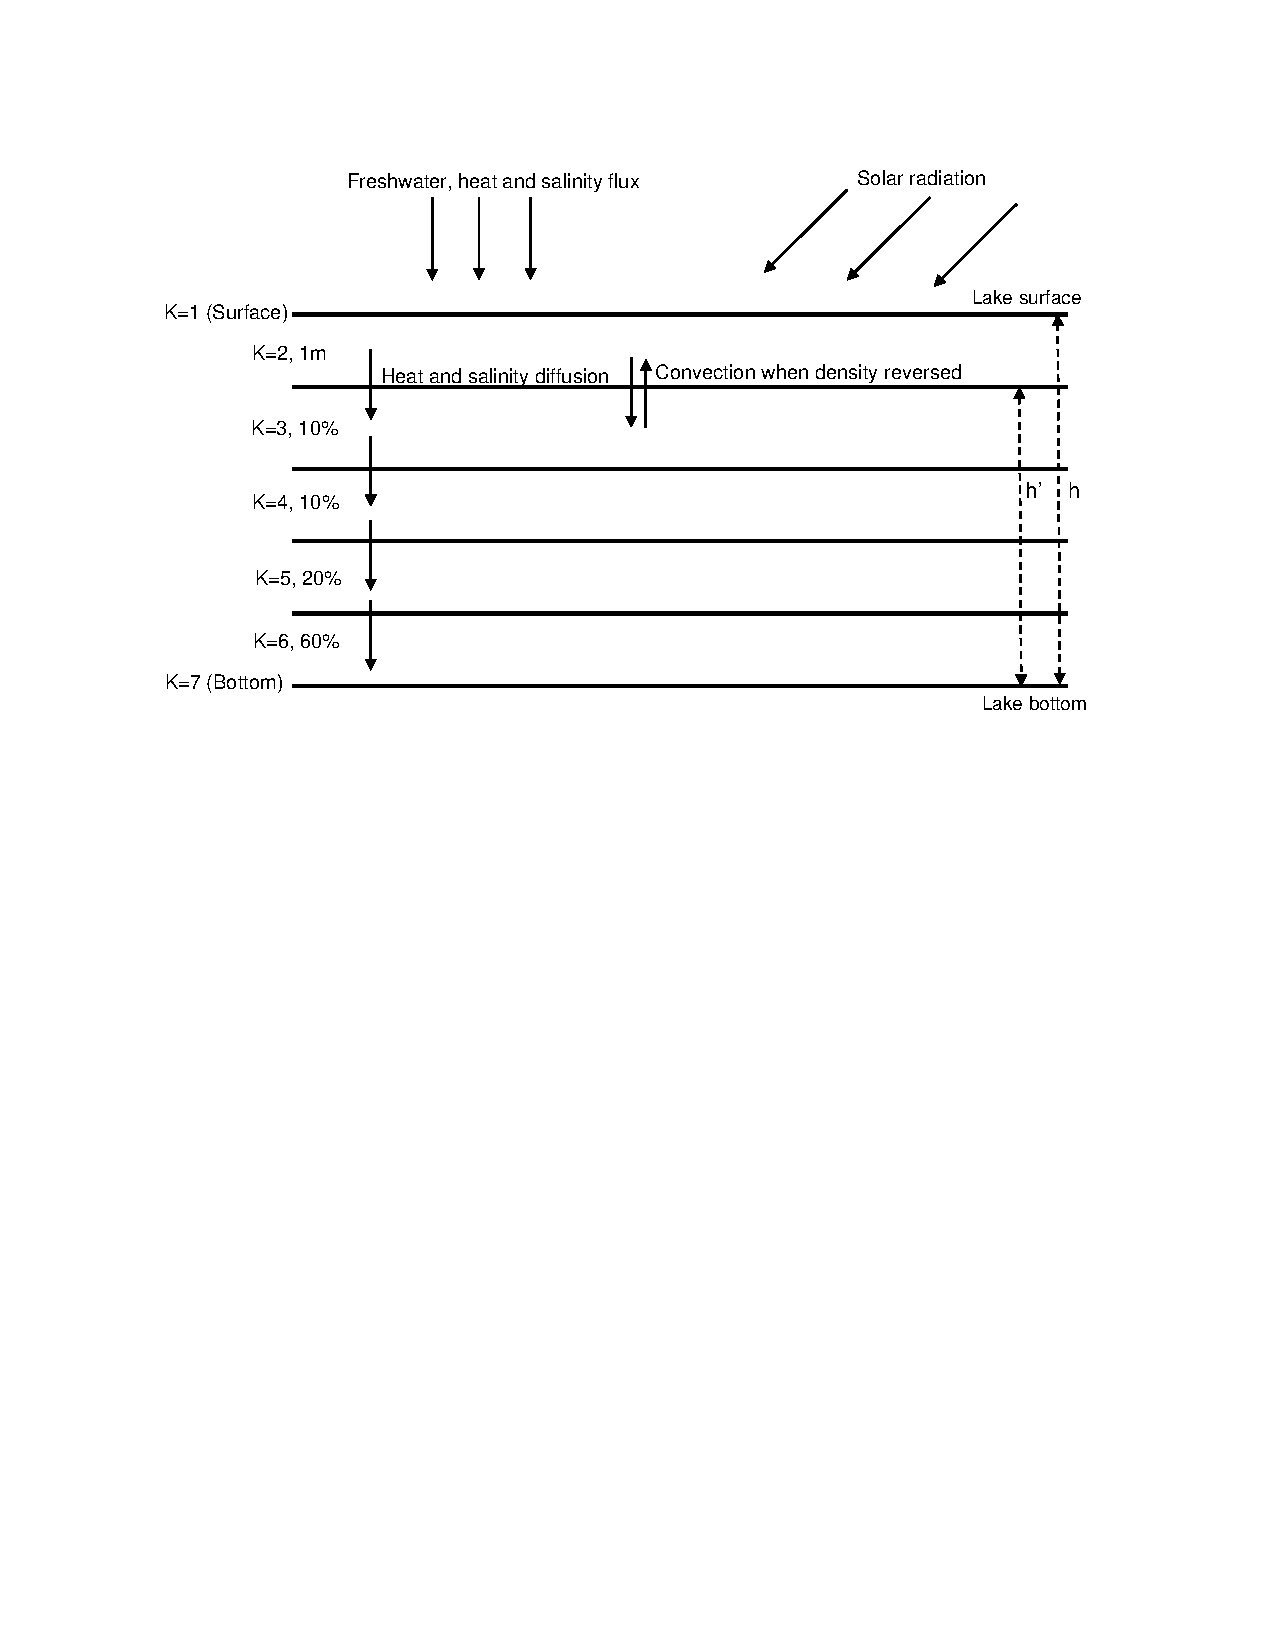
\includegraphics{descript/Lake_11-1.pdf}
\caption{The layer of the water column}
\end{figure}

Firstly, the thickness of the first layer (k=2) is fixed and represented as \(D_{1}\), and \(D_{1}\) is set to 100 cm. Therefore, the thickness of the first layer can be described as: \begin{eqnarray}
D(2)=D_{1}
\end{eqnarray} The thicknesses of the other layers (k=3, 4, 5, 6) are calculated based on the ratio of the remaining thickness of the water column. Using \(h\) to represent the total depth of the water column,
and the thickness of the remaining water column (\(h'\)) excluding the top layer is presented by: \begin{eqnarray}
h'=h-D_{1}
\end{eqnarray} and thickness (\(D(k)\)) of the remaining layer (k=3, 4, 5, 6) can be represented as: \begin{eqnarray}
D(k)=S(k)h'
\end{eqnarray} The ratio (\(S(k)\)) of layer 3 to 6 are 0.1, 0.1. 0.2, and 0.6, respectively. Therefore, the thermal change of the k-th layer by vertical diffusion can be represented as the flux difference
between upper layer \(J_{k-1, k}\) and lower layer \(J_{k, k+1}\): \begin{eqnarray}
F_{D}(k)=J_{k-1,k}-J_{k,k+1}=K_{V}(k)\frac{T(k-1)-T(k)}{\frac{D(k-1)+D(k)}{2}}-K_{V}(k+1)\frac{T(k)-T(k+1)}{\frac{D(k)+D(k+1)}{2}}
\end{eqnarray}

The above equations apply to salinity as well.

\hypertarget{time-integration-of-the-tracer-equations}{%
\subsubsection{Time integration of the tracer equations}\label{time-integration-of-the-tracer-equations}}

\textbf{Input}

\begin{longtable}[]{@{}llll@{}}
\toprule
Meaning & Character & In code & Unit \\
\midrule
\endhead
The vertical component of diffusive tracer flux & \(F_{D}\) & ADT & \(^{o}C\)/s \\
Minimum depth of the lake & \(h_{min}\) & HXMIN & m \\
Heat flux & \(F_{T}\) & FT (1) & \(^{o}C\)/s \\
Freshwater flux & \(F_{W}\) & FT(2) & cm/s \\
Absorbed shortwave solar radiation & \(S_{r}\) & SWABS & \\
Salt flux & \(F_{S}\) & FS & \\
Timestep & \(\Delta t\) & TS & s \\
Surface-type fraction (lake) & \(R_{lake}\) & LKFRAC & - \\
\bottomrule
\end{longtable}

\textbf{Output}

\begin{longtable}[]{@{}llll@{}}
\toprule
Meaning & Character & In code & Unit \\
\midrule
\endhead
Lake water deficiency & \(V_{D}\) & XHD & cm \\
\bottomrule
\end{longtable}

This part introduces the update of water temperature and salinity of each layer due to the diffusion, freshwater flux, and absorption of solar radiation. The source code is included in ENTRY
{[}SLVTRCL{]} (in SUBROUTINE: {[}LAKEPO{]} of lakepo.F).

Heat diffusion is first considered. According to Fick's second law, the temperature (salinity as well) change of k-th layer follows: \begin{eqnarray}
\frac{\partial T}{\partial t}=K_{V}(k)\frac{\partial^2 T}{\partial z^2}
\end{eqnarray} where \(z\) is the vertical distance. The equation is implicitly (backward-in-time) integrated, and obtains: \begin{eqnarray}
\frac{T^{n+1}(k)-T^{n}(k)}{\Delta t}=\frac{K_{V}(k)\frac{T^{n+1}(k-1)-T^{n+1}(k)}{\frac{D(k-1)+D(k)}{2}}-K_{V}(k+1)\frac{T^{n+1}(k)-T^{n+1}(k+1)}{\frac{D(k)+D(k+1)}{2}}}{D(k)}
\end{eqnarray} The Tridiagonal Matrix Algorithm (also known as the Thomas Algorithm) is used to solve the equation, the following equation is constructed: \begin{eqnarray}
A_{A}(k)F_{D}(k-1)+A_{B}(k)F_{D}(k)+A_{C}(k)F_{D}(k+1)=F_{D}(k)
\end{eqnarray} where \begin{eqnarray}
A_{A}(k)=-\frac{K_{V}(k)}{\frac{D(k-1)+D(k)}{2}}\Delta t
\end{eqnarray}

\begin{eqnarray}
A_{C}(k)=-\frac{K_{V}(k+1)}{\frac{D(k)+D(k+1)}{2}}\Delta t
\end{eqnarray}

\begin{eqnarray}
A_{B}(k)=D(k)-A_{A}(k)-A_{C}(k)
\end{eqnarray}

Then, the new coefficient of the Tridiagonal Matrix Algorithm can be constructed: \begin{eqnarray}
A_{c}'(k)=\left\{\begin{matrix}
\frac{A_{C}}{A_{B}},&k=&2\\\frac{A_{C}}{A_{B}-A_{A}(k)A_{C}'(k-1)}, &k=&3, 4, 5, 6
\end{matrix}\right.
\end{eqnarray}

\begin{eqnarray}
A_{D}'(k)=\left\{\begin{matrix}
\frac{F_{D}(k)}{A_{B}(k)}, &k=&2\\\frac{F_{D}(k)-A_{A}(k)A_{D}'(k-1)}{A_{B}-A_{A}(k)A_{C}'(k-1)}, &k=&3, 4, 5, 6
\end{matrix}\right.
\end{eqnarray}

Then, the vertical diffusion term can be obtained: \begin{eqnarray}
F_{D}(k)=\left\{\begin{matrix}
A_{D}'(k), &k=&6\\A_{D}'(k)-A_{C}'(k)F_{D}(k+1), &k=&2, 3, 4, 5
\end{matrix}\right.
\end{eqnarray}

The water temperature of each layer is updated as: \begin{eqnarray}
T_{k}=T(k)+F_{D}(k)\Delta t
\end{eqnarray} After solving diffusive changes of tracers, the effect of heat, salinity, and freshwater fluxes at the lake surface is taken into account. Since the height of the water column changes with the
freshwater flux, tracers at each layer should be re-estimated. It worth noting that a minimum depth threshold \(h\_{min}\) is set, which means the lake depth can not be lower than this value. When
surface freshwater flux \(F_{W}\) (positive upward, i.e., the lake level is lowered when \(F_{W}\) \textgreater{} 0) is imposed, and the change of the water column for each time step can be
represented as: \begin{eqnarray}
h_{D}=-F_{W}\Delta t
\end{eqnarray} and the lake water deficiency (when lake depth \(h\) is smaller than the minimum threshold \(h_{min}\)) can be represented as: \begin{eqnarray}
V_{D}=max(h_{min}-h-h_{D}, 0)\times R_{lake}
\end{eqnarray} where \(R_{lake}\) is the lake fraction of the grid. Therefore, the change of the lake depth is finalized as: \begin{eqnarray}
h_{D}=max(h_{D}, h_{min}-h)
\end{eqnarray} and the lake depth is updated: \begin{eqnarray}
h=h+h_{D}
\end{eqnarray}

Due to the added freshwater, the depth of each lake layer has been changed, so the water temperature of each layer is updated as well. The update of depth and water temperature starts from the bottom
layer. When \(h_{D}\) \textgreater{} 0, the bottom of the k-th layer in the z coordinate is raised by: \begin{eqnarray}
\Delta z_{B}^{k}=(1-\sum_{l=2}^{k}S(k))h_{D}
\end{eqnarray} where \(S(k)\) is the vertical depth proportion of the k-th layer, and its top is raised by: \begin{eqnarray}
\Delta z_{T}^{k}=(1-\sum_{l=2}^{k-1}S(k))h_{D}
\end{eqnarray} where the following equation holds: \begin{eqnarray}
\Delta z_{k}^{T}=\Delta z_{k-1}^{B}
\end{eqnarray} Therefore, the temperature of the k-th (k=3, 4, 5, 6) layer becomes: \begin{eqnarray}
T(k)=\frac{T(k)D(k)-T(k)\Delta z_{k}^{B}+T(k-1)\Delta z_{k}^{T}}{D(k)}
\end{eqnarray} The temperature of the first layer (k=2) becomes: \begin{eqnarray}
T(2)=\frac{T(2)D(2)-T(2)\Delta z_{2}^{B}+T(2)\Delta z_{2}^{T}+F_{T}\Delta t}{D(2)}
\end{eqnarray} where \(F_{T}\) is the heat flux of the freshwater added to the lake, and for salinity, the salinity flux is \(F_{S}\).

When \(h_{D}\) \textless{} 0, on the other hand, the bottom of the k-th level is lowered by \(\Delta z_{k}^{B}\), and its top is lowered by \(\Delta z_{k}^{T}\). In this case, the above tracer
equations for the k-th layer (k=3, 4, 5, 6) and the first layer (k=2) become: \begin{eqnarray}
T(k)=\frac{T(k)D(k)-T(k)\Delta z_{k}^{T}+T(k+1)\Delta z_{k}^{B}}{D(k)}
\end{eqnarray}

and \begin{eqnarray}
T(2)=\frac{T(2)D(2)-T(2)\Delta z_{2}^{T}+T(3)\Delta z_{2}^{B}+F_{T}\Delta t}{D(2)}
\end{eqnarray} Finally, the absorption of solar radiation is considered. The temperature of each layer is updated as: \begin{eqnarray}
T(k)=T(k)+\frac{S_{r}\times C_{sr}(k)}{D(k)\rho _{0}C_{P0}}\Delta t
\end{eqnarray} where \(S_{r}\) represents the solar radiation, and \(C_{sr}\) represents the absorption proportion of each layer. \(\rho_{0}\) and \(C_{p0}\) are density and specific heat capacity of water, and
their values are set as 1 g/cm3 and 3.99×107 erg/g/K, respectively. \(C_{sr}\) is calculated based on the depth of each layer, the transitivity \(T_{rs}(k)\) at depth \(D_{t}(k)\) can be represented
as: \begin{eqnarray}
T_{rs}=R_{r}\times e^{-\frac{D_{t}(k)}{z_{1}}}+(1-R_{r})\times e^{-\frac{D_{t}(k)}{z_{2}}}
\end{eqnarray} where \(R_{r}\), \(z_{1}\), and \(z_{2}\) are three parameters, and their values are 0.58, 35, and 2300, respectively.

\(D_{t}(k)\) represent the total depth of the bottom of k-th layer: \begin{eqnarray}
D_{t}(k)=\sum_{l=2}^{k}D(k)
\end{eqnarray} Therefore, \(C_{sr}\) can be represented as: \begin{eqnarray}
C_{sr}(k)=\left\{\begin{matrix}
1-T_{rs}(k), &k=&2\\T_{rs}(k-1)-T_{rs}(k), &k=&3, 4, 5
\\ 1-\sum_{l=2}^{5}C_{sr}(k), &k=&6
\end{matrix}\right.
\end{eqnarray}

\hypertarget{the-vertical-convection}{%
\subsubsection{The vertical convection}\label{the-vertical-convection}}

This part introduced the vertical convection of the water between different layers, and the source code is included in ENTRY {[}OVTURNL{]} (in SUBROUTINE: {[}LAKEPO{]} of lakepo.F).

A classical, still widely used method-convective adjustment, which unstable water column is artificially homogenized with conserving heat and salt. MATSIRO 6 employs the convective adjustment for the
standard choice, but its algorithm is not the pairwise adjustment. It is summarized as follows:

\begin{enumerate}
\def\labelenumi{(\arabic{enumi})}
\item
  Set the index \(K_{s}\)=2 (the first layer), indicating the start level of the convective adjustment, and set the index \(K_{e}\)=3 (the second layer), indicating the level where instability is
  currently judged.
\item
  Compare potential density (\(\rho\)) of the (\(K_{e}\)-1)-th and \(K_{e}\)-th layers. If instability (\(\rho_{Ke-1}\)\textgreater{} \(\rho_{Ke}\)) is found, go to step 3, and if instability is not
  found, go to step 4.
\item
  Mix the water column between the \(K_{s}\)-th layer and \(K_{e}\)-th layer. Increase \(K_{e}\) by 1, and if the (new) \(K_{e}\) is greater than 6 (the bottom layer), the convection procedure ends.
  If not, go back to step 2 with the new \(K_{e}\).
\item
  Set \(K_{s}\)=\(K_{e}\), and increase \(K_{e}\) by 1. Increase \(K_{e}\)by 1, and if the (new) \(K_{e}\) is greater than 6 (the bottom layer), the convection procedure ends. If not, go back to step
  2 with new \(K_{s}\) and \(K_{e}\).
\end{enumerate}

The water density is calculated by: \begin{eqnarray}
\rho =999.842594+6.793952\times 10^{-2}\times T-9.095290\times 10^{-3}\times T^{2}+1.001685\times
      10^{-4}\times T^{3}\\ -1.120083\times 10^{-6}\times T^{4}+6.536332\times 10^{-9}\times T^{5}
\end{eqnarray}

where \(T\) represents temperature. When instability happens, the water column between the \(Ks\) layer and \(K_{e}\) will convect and mix, and the water temperature of these layers will be identical
and are updated as: \begin{eqnarray}
T(K_{s}, ..., K_{e})=\frac{\sum_{k=K_{s}}^{K_{e}}D(k)T(k)}{\sum_{k=K_{s}}^{K_{e}}D(k)}
\end{eqnarray}

\hypertarget{lake-river-coupling}{%
\subsection{Lake river coupling}\label{lake-river-coupling}}

The inflow rate from the river to the lake, \(R_{in}\) \([cm/s]\), is calculated as follws.

\begin{eqnarray}
    R_{in} = H_{riv} / (\tau_{riv} * 86400)
\end{eqnarray}

where \(H_{riv}\) \([cm]\) is grid average river water depth, \(\tau_{riv}\) is a time constant, and 86400 is a unit conversion coefficient. \(\tau_{riv}\) is set to 1 day by default. \(H_{riv}\) is
derived the following equation.

\begin{eqnarray}
    H_{riv} = w_{riv} / \rho_w * 100
\end{eqnarray}

where \(w_{riv}\) is the river water volume \([kg/m^2]\), \(\rho_w\) is the density of water, and 100 is the coefficient for unit conversion.

When water depth \(H [cm]\) of a lake becomes deeper than the upper limit \(H_{max}\), water outflows into river channel. The outflow rate to the river, \(R_{out} [cm/s]\), is diagnosed as follows.

\begin{eqnarray}
    R_{out} = (H - H_{max}) / ( \tau_{lake} * 86400 )
\end{eqnarray}

The \(H_{max} [cm]\) is, by default, the climatology of lake depth + 10 m. \(\tau_{lake}\) is a time constant, which is also set to 1 day.

Finally, \(R_{out}\) is added to runoff from land and given to the river.

\hypertarget{wetland}{%
\section{Wetland}\label{wetland}}

\hypertarget{outline-of-wetland-scheme}{%
\subsection{Outline of wetland scheme}\label{outline-of-wetland-scheme}}

A snow-fed wetland scheme, in which snowmelt can be stored with consideration of sub-grid terrain complexity, is incorporated as a sub-module of TOPMODEL (when \# ifdef OPT\_SW\_STORAGE in SUBROUTINE:
{[}MATROF{]} in matrof.F is active) in MATSIRO 6 to represent the wetland-related process in the middle and high latitudes grid with snowmelt (Nitta et al., 2015, 2017) (Fig. 12-1). The wetland scheme
has two major effects: 1) the storage of part of the surface water and delay of runoff to rivers, 2) an increase in land surface wetness thus enhancing the evaporation in water-limited regimes.

With the wetland scheme, when snowmelt occurs, instead of all the generated surface runoff flows directly to the rivers, only a part of the surface runoff flows into the rivers and the remaining part
of the surface runoff is stored by the added tank (also known as the snow-fed wetland). Then, the stored water in the wetland is then re-added to the water input of soil combining with other kinds of
water inputs (Fig. 12-1). In the current version, only snow-fed wetlands are considered, and more types of wetland schemes will be added in the future version.

\begin{figure}
\centering
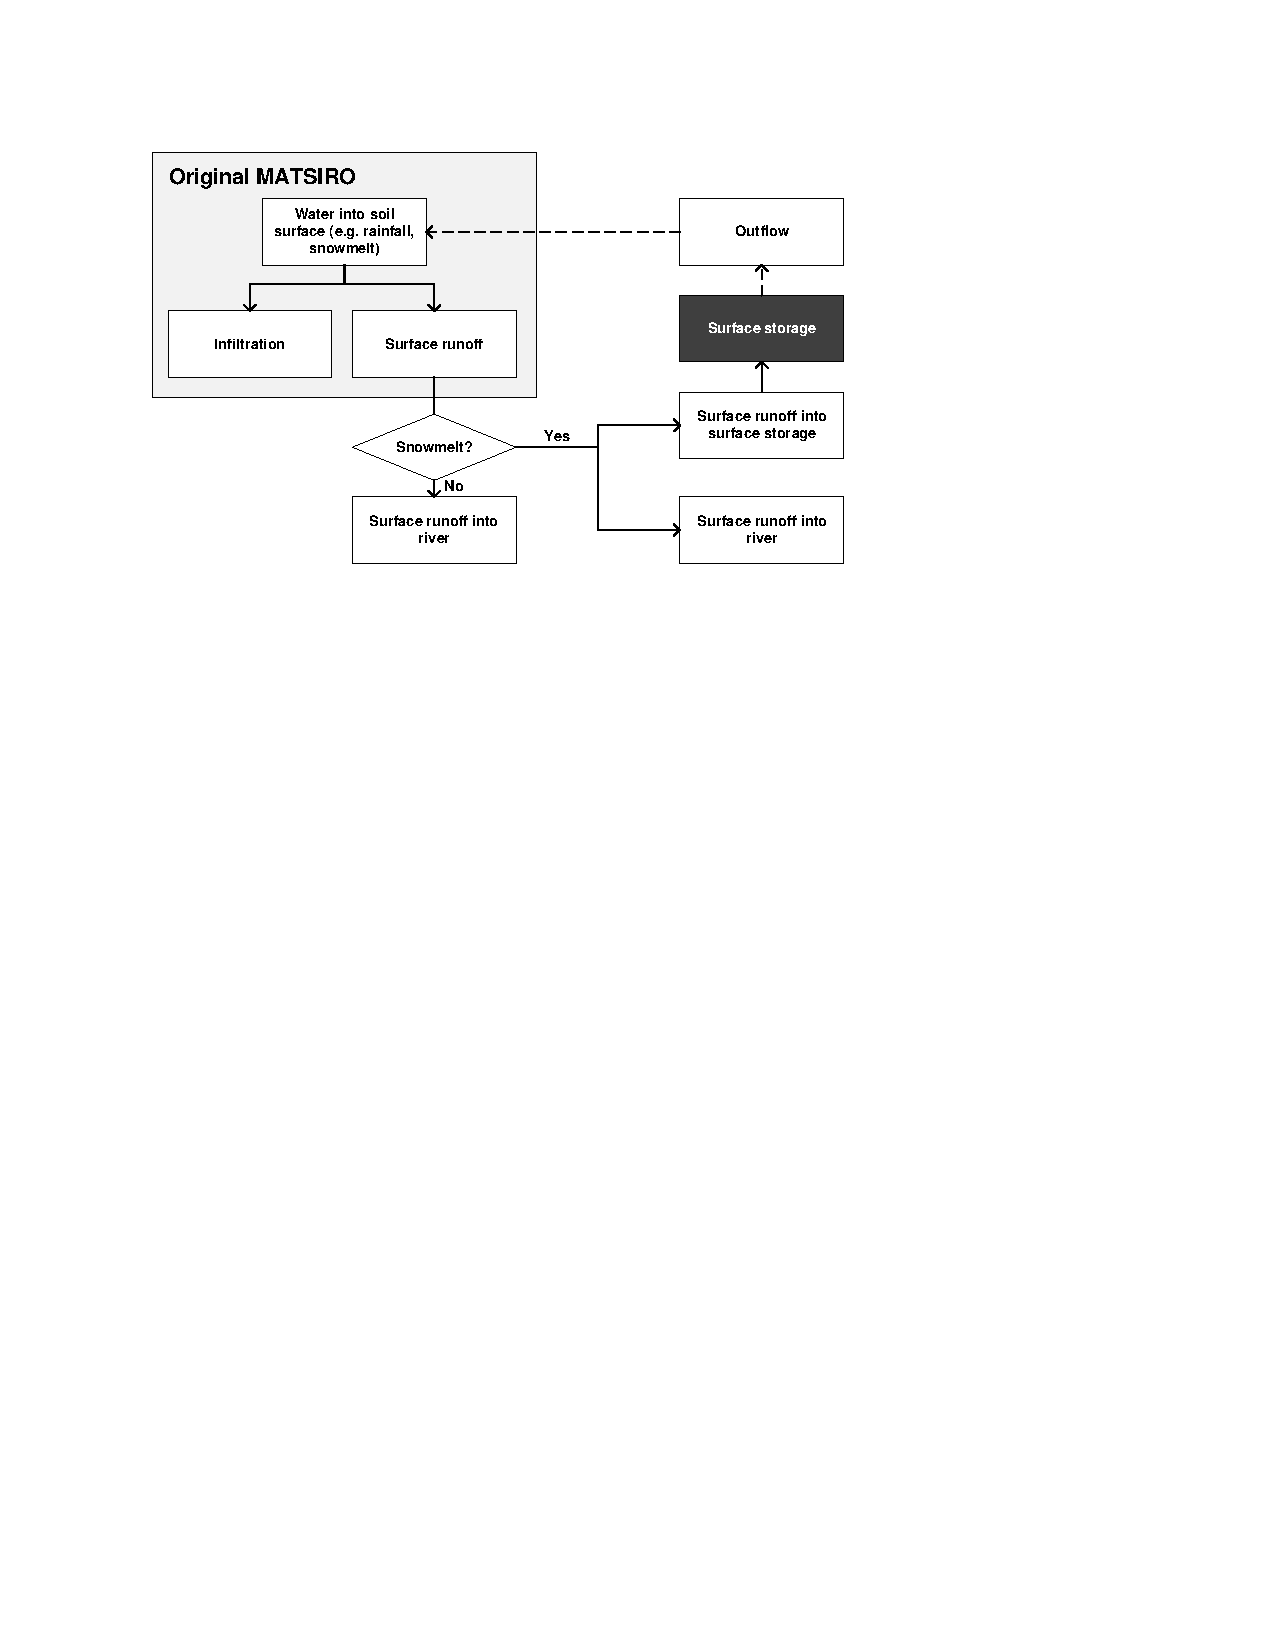
\includegraphics{descript/Wetland_12-1.pdf}
\caption{Flowchart of the wetland scheme in the MATSIRO 6}
\end{figure}

\hypertarget{inflow-and-outflow-of-the-wetland}{%
\subsection{Inflow and outflow of the wetland}\label{inflow-and-outflow-of-the-wetland}}

The inflow of the wetland comes from the fraction of the surface runoff, and its amount is determined by the tunable parameter \(\alpha\). The outflow from the wetland is calculated using a time
constant \(\beta\) and the wetland storage \(S\), consequently flowing into the soil surface. Therefore, the update of the wetland storage \(S\) at each time step can be represented as:

\begin{eqnarray}
\frac{S^{\tau +1}-S^{\tau }}{\Delta t}=-\frac{S}{\beta}+(1-\alpha )R_{s}
\end{eqnarray}

where \(R_{s}\) is surface runoff calculated as a total of \(Ro_{s}\) (saturation excess runoff), \(Ro_{i}\) (infiltration excess runoff), and \(Ro_{o}\) (overflow of the uppermost soil layer);
\(\tau\) is time; and \(\alpha\) and \(\beta\) are parameters related to the inflow and outflow of the wetland storage, respectively.

\(\beta\) is a spatially dependent time constant, and can be calculated using a function of the standard deviation of elevation above sea level:

\begin{eqnarray}
\beta =max(\beta_{0}(1-min(\sigma_{z}(x),\sigma_{z max})/\sigma_{z max}), \Delta t)
\end{eqnarray}

where \(\beta_{0}\) is the maximum of the time constant, \(\sigma _{z}\) is the standard deviation of elevation above sea level within each grid at point \(x\), and \(\Delta t\) is the time step of
the model. The parameter \(\sigma_{z}\) is a physical parameter calculated by the topography dataset, with a higher spatial resolution than the simulation, and \(\beta_{0}\), \(\sigma_{zmax}\), and
\(\alpha\) are tunable parameters. These parameter values were determined based on sensitivity simulations using an offline land model with perturbed parameters; 1 month, 200m, and 0.1 were chosen as
the most appropriate values for \(\beta_{0}\), \(\sigma _{zmax}\), and \(\alpha\), respectively (Nitta et al., 2015).

\hypertarget{storage-of-the-surface-runoff}{%
\subsection{Storage of the surface runoff}\label{storage-of-the-surface-runoff}}

The ratio of total surface runoff that flows directly to the rivers is controlled by parameter \(\alpha\). Therefore, the actual runoff flows into rivers \(Ro\) changes to:

\begin{eqnarray}
Ro=(Ro_{s}+Ro_{i}+Ro_{o})\times \alpha + Ro_{b}
\end{eqnarray}

where \(\alpha\) is the inflow parameter (see 12.1); \(Ro_{s}\) is the saturation excess runoff (Dunne runoff), \(Ro_{i}\) is the infiltration excess runoff (Horton runoff), and \(Ro_{o}\) is the
overflow of the uppermost soil layer, and all these three kinds of runoff make up the total surface runoff, and \(Ro_{b}\) is the groundwater runoff (section 7.3).

\hypertarget{water-input-of-soil-surface}{%
\subsection{Water input of soil surface}\label{water-input-of-soil-surface}}

The outflow from the wetland storage is re-added to the water input of the soil surface, combining with the original water input (e.g.~precipitation that passes through canopy gaps, water drops from
the canopy, and snowmelt water). Therefore, the updated soil water input \(WI_{soil,total}\) of each time step can be represented as:

\begin{eqnarray}
WI_{soil,total}=Pr_{c}^{**}+Pr_{l}^{**}-Ro_{s}-Ro_{i}+\frac{S}{\beta }\Delta t
\end{eqnarray}

where \(Pr_{c}^{**}\) represents the convective rainfall, \(Pr_{l}^{**}\) represents the non-convective rainfall, \(S\) represents the wetland storage, \(\beta\) represents the outflow parameter of
the wetland, and \(\Delta t\) is the time step.

\hypertarget{tile-scheme}{%
\section{Tile scheme}\label{tile-scheme}}

MATSIRO employs a tile treatment of the land surface to represent the subgrid land surface types, so as to partially mimic the behavior at a higher resolution. The tile scheme is demonstrated in
ENTRY:{[}LNDFLX{]} and {[}LNDSTP{]} (in SUBUROUTINE: {[}MATSIRO{]} of matdrv.F), and the variables and parameters are introduced as follows:

\begin{itemize}
\tightlist
\item
  Output variables
\end{itemize}

\begin{longtable}[]{@{}llll@{}}
\toprule
Variable & Description & Code & Units \\
\midrule
\endhead
\(F\) & Fluxes at the land surface & MATFLX & - \\
\(F_{lake}\) & Fluxes at the land surface of lake & - & - \\
\(F_i(i=1,2)\) & Fluxes at the land surface of potential vegetation and cropland & - & - \\
\bottomrule
\end{longtable}

\begin{itemize}
\tightlist
\item
  Parameters
\end{itemize}

\begin{landscape}

\begin{longtable}[]{@{}llll@{}}
\toprule
PARAMETER & Description & Code & Units \\
\midrule
\endhead
\(f_{lake}\) & Fractional weight of lake in grid & LKFRAC & - \\
\(f_i(i=1,2)\) & Fractional weight of potential vegetation and cropland in grid & SFFRAC & - \\
\(f_i^"(i=1,2)\) & Sub-fractional weight of potential vegetation and cropland on land & SFFRAC1 & - \\
\bottomrule
\end{longtable}

\end{landscape}

Basically, one land surface grid is divided into three tiles in the control run --- lake, potential vegetation and cropland:

\begin{enumerate}
\def\labelenumi{\arabic{enumi}.}
\tightlist
\item
  There are both snow-covered and snow-free fractions in each tile;
\item
  The surface heat and water fluxes over lakes have been calculated as one of the tiles in a grid;
\item
  Both potential vegetation and cropland tiles consist of six soil layers, up to three snow layers, and a single canopy layer, driving predictions of the temperature and amount of water in the canopy,
  soil, and snow;
\item
  Potential vegetation is defined according to the vegetation types of the Simple Biosphere Model 2 (SiB2; Sellers et al.~1996) scheme and has 10 categories including land ice. There is no wetland
  category for land cover in the original SiB2 vegetation types or soil types.
\end{enumerate}

All the prognostic and diagnostic variables are calculated in each tile, and the fluxes at the land surface \(F\) are averaged: \begin{eqnarray}
F=F_{lake}f_{lake}+\sum_{i=1}^nF_if_i
\end{eqnarray}

\begin{eqnarray}
f_i=f_i^"(1-f_{lake})
\end{eqnarray}

\begin{eqnarray}
\sum_{i=1}^nf_i^"=1
\end{eqnarray}

where n is 2, \(F_{lake}\), \(F_1\) and \(F_2\) denote fluxes at the land surface of lake, potential vegetation and cropland, \(f_{lake}\), \(f_1\) and \(f_2\) denote their corresponding fractional
weights (the sum of \(f_{lake}\), \(f_1\) and \(f_2\) always equals 1), \(f_1^"\) and \(f_2^"\) denote the sub-fractional weights of potential vegetation and cropland on land (note that \(f_1^"\) and
\(f_2^"\) have been utilized as boundary condition data in MATSIRO6), respectively.

By default, tile scheme is applied in land surface type, but it can be used for multiple purposes.

\hypertarget{references}{%
\section{References}\label{references}}

\begin{itemize}
\item
  Ball, J. T., 1988: An analysis of stomatal conductance. Ph.D.~thesis, Stanford University, 89 pp.
\item
  Beven, K. J., and M. J. Kirkby, 1979: A physically based variable contributing area model of basin hydrology, {Hydrol. Sci. Bull.}, {\textbf{24}}, 43--69.
\item
  Clapp, R. B., and G. M. Hornberger, 1978: Empirical equations for some soil hydraulic properties. {Water Resour. Res.}, {\textbf{14}}, 601--604.
\item
  Collatz, G. J., J. A. Berry, G. D. Farquhar, and J. Pierce, 1990: The relationship between the Rubisco reaction mechanism and models of leaf photosynthesis. {Plant Cell Environ.}, {\textbf{13}},
  219--225.
\item
  Collatz, G. J., J. T. Ball, C. Grivet, and J. A. Berry, 1991: Physiological and environmental regulation of stomatal conductance, photosynthesis and transpiration: A model that includes a laminar
  boundary layer. {Agric. For. Meteor.}, {\textbf{54}}, 107--136.
\item
  Collatz, G. J., M. Ribas-Carbo, and J. A. Berry, 1992: Coupled Photosynthesis-Stomatal Conductance Model for leaves of TERM00000 plants. {Aust. J. Plant. Physiol.}, {\textbf{19}}, 519--538.
\item
  Farquhar, G. D., S. von Caemmerer, and J. A. Berry, 1980: A biochemical model of photosynthetic TERM00001 fixation in leaves of TERM00002 species. {Planta}, {\textbf{149}}, 78--90.
\item
  Kondo, J., and T. Watanabe, 1992: Studies on the bulk transfer coefficients over a vegetated surface with a multilayer energy budget model. {J. Atmos. Sci}, {\textbf{49}}, 2183--2199.
\item
  Nitta, T., Yoshimura, K., and Abe-Ouchi, A., 2015: A Sensitivity Study of a Simple Wetland Scheme for Improvements in the Representation of Surface Hydrology and Decrease of Surface Air Temperature
  Bias. {Journal of Japan Society of Civil Engineers, Ser.B1 (Hydraulic Engineering)}, {\textbf{71(4)}}, 955-960.
\item
  Nitta, T., Yoshimura, K., and Abe-Ouchi, A., 2017: Impact of Arctic Wetlands on the Climate System: Model Sensitivity Simulations with the MIROC5 AGCM and a Snow-Fed Wetland Scheme. { Journal of
  Hydrometeorology}, {\textbf{18(11)}}, 2923-2936.
\item
  Rutter, B., A. J. Morton, and P. C. Robins, 1975: A predictive model of rainfall interception in forests. II. Generalization of the model and comparison with observations in some coniferous and
  hardwood stands. {J. Appl. Ecol.}, {\textbf{12}}, 367--380.
\item
  Sellers, P. J., D. A. Randall, G. J. Collatz, J. A. Berry, C. B. Field, D. A. Dazlich, C. Zhang, G. D. Collelo, and L. Bounoua, 1996: A revised land surface parameterization (SiB2) for atmospheric
  GCMs. Part I: Model formulation. {J. Climate}, {\textbf{9}}, 676--705.
\item
  Sellers, P. J., Meeson, B. W., Closs, J., Collatz, J., Corprew, F., Dazlich, D., Hall, F. G., Kerr, Y., Koster, R., Los, S., Mitchell, K., McManus, J., Myers, D., Sun, K.-J, and Try, P.: The ISLSCP
  Initiative I global datasets: surface boundary conditions and atmospheric forcings for land-atmosphere studies, B. Am. Meteorol. Soc., {\textbf{77}}, 1987--2006, 1996.
\item
  Sivapalan, M., K. Beven, and E. F. Wood, 1987: On hydrologic similarity. 2, A scaled model of storm runoff production. {Water Resour. Res}, {\textbf{23}}, 2266--2278.
\item
  Stieglitz, M., D. Rind, J. Famiglietti, and C. Rosenzweig, 1997: An efficient approach to modeling the topographic control of surface hydrology for regional and global climate modeling. {J.
  Climate}, {\textbf{10}}, 118--137.
\item
  Watanabe, T., 1994: Bulk parameterization for a vegetated surface and its application to a simulation of nocturnal drainage flow. {Boundary-Layer Met.}, {\textbf{70}}, 13--35.
\item
  Wiscombe, W. J., and S. G. Warren, 1980: A model for the spectral albedo of snow. I. Pure snow. {J. Atmos. Sci.}, {\textbf{37}}, 2712--2733.
\item
  Hirabayashi, Y., Global analysis on long term variations of extreme river discharge, The University of Tokyo, Doctoral degree thesis, 2004
\item
  渡辺力・大谷義一, 1995: キャノピー層内の日射量分布の近似計算法. {農業気象}, {\textbf{51}}, 57--60.
\end{itemize}

	%
	%
\end{document}
